%!TEX root = ../thesis.tex
\chapter{Coregistration of High Resolution Rat Histology}
% If you like chapter abstracts ...
\dblspace
\begin{quote}{\em %!TEX root = ../thesis.tex
Adjacent histological slices can be coregistered accurately and lead to smooth image volumes, owing to their close morphological resemblance and their similar intensity spectra. However, volumes constructed from serial histology registration do not reflect the true 3-dimensional tissue geometry. Registration of histology to a set of coherent reference images yields an authentic geometry on the organ scale, yet the lower resolution and differing modality of the references leads to noisy, jagged volumes on the microstructural scale.

We present in this chapter an algorithm to align neighbouring slices accurately and smoothly without disturbing large scale tissue shape, based on a microscopic model of diffusion. We develop a mathematically sound and general framework of transformational diffusion, based on the Lie theory of continous groups. Using synthetic geometries of cardiac tissue with artificial noise, we demonstrate a robust and precise dispersion of information between slices on a configurable range of scales, recovering volumes which are orders of magnitude smoother and which have maintained faithfully the underlying geometrical signal. We apply the algorithm to the volumes from Chapter~\ref{cha:coregistration_of_high_resolution_rat_histology}, first globally and then again to the region around an epicardial vessel. Previously indiscernible microvasculature and sheet structure become patent. Pericardium and epicardial vessel segmentations show that displacement abberations between adjacent slices of the order of 400$\mu$m are reduced by two orders of magnitude. The methods presented here outperform any such method to reconstruct histological volumes based on reference images currently in the literature. Finally, we discuss several interesting applications and refinements that might be made to the algorithm in specific cases, including anisotropic diffusion based on image features or inter-slice transform magnitudes. The results of this work are presented Computational Methods in Systems Biology 2012 \cite{Gibb2012}, and the work in Chapter~\ref{cha:coregistration_of_high_resolution_rat_histology} and this Chapter will be published in detail in IEEE Transactions on Medical Imaging.
}\end{quote}

CONFIRMATION REPORT
\section{Aims}
  MOTIVATION, PROBLEMS, AIMS
  
  Having shown in an idealised geometry that fibre direction could have a significant effect on propagation, the challenge is set to characterise cardiac tissue at sufficient detail to resolve both fibre direction and other microstructure. Cell type distribution, the shape of tissue boundaries, the Purkinje fibre network, sheet structure and vasculature all affect macroscopic wave propagation. In this section we will lay the foundations for investigating these effects by registering high-resolution histological data with MRI images. Following on from the work touched on in section~\ref{sec:cardiac_tissue_can_be_accurately_characterised_with_high_resolution_data} by \cite{Mansoori2007}, we will first examine more closely the sources of deformation introduced by the image acquisition process. A brief summary of computational tools will follow, before an overview of the registration method. We end with a discussion of the progress so far and some thoughts on what the finished pipeline will yield.
  
  
  
  Intro/Motivation
  People have tried to align block faces, but can't use certain dyes, transmission problems, lo res with Lo res data.
  People have tried to align hires stuff, but we know that this is not consistent.
  ASK VICENTE FOR REFS. MARK BOYETT FIRST AUTHOR OF ONE PAPER. ASK BECKY FOR INTRO/METHODS PAPERS.
  First attempt to use both sets of data to make coherent hires dyed segmented etc.
  
  \emph{This paper will be composed of four main sections: an overview of experimental methods, a review of the architecture of the library developed to register the raw data, a comparison of algorithms and their utility to this end, and finally the results of successful registration, with several colour figures providing visual validation of the methods.}
  
  The aim of this chapter is to develop an automated pipeline to register high resolution rat cardiac datasets robustly and accurately, and generate coherent subcellular resolution 3-D cardiac histological images.  Approximately three full rat heart datasets will be processed through the pipeline to provide registered volumes. These images will serve both as an authoritative anatomical reference, and as the basis for anatomically based models in simulation studies.
  
\section{Methods} % (fold)
\label{sec:methods}
  INTRODUCTORY PARAGRAPH
  
  \subsection{Image Acquisition} % (fold)
  \label{sub:image_acquisition}
    Hearts were isolated from female rats and cannulated via the aorta to a Langendorff perfusion system, in a similar manner to that presented in \cite{Burton2006}. The hearts were then fixed and stabilised in agar, and 26.4 x 26.4 x 26.4$\mu$m MRI scans were performed. The hearts were immersed in increasing concentrations of alcohol, in order to dehydrate them before embedding them in black wax. The wax blocks were then serially sectioned at 10$\mu$m thickness using a microtome. An image of the top surface of the block was taken with 25$\mu$m resolution after each slicing. Every 5th section was Trichrome stained, labelling connective tissue bluish-green, myocytes pinkish-red and nuclei blue-black. Each slice was relaxed and re-hydrated, before histology imaging was performed using a 5x objective with 1.1$\mu$m resolution. Examples of the block face and slice images is displayed in Figures~\labelcref{fig:original_lores_images,fig:original_hires_images}, respectively.
		
		\begin{figure}[htbp]
		  \centering
		  \subfigure[][]{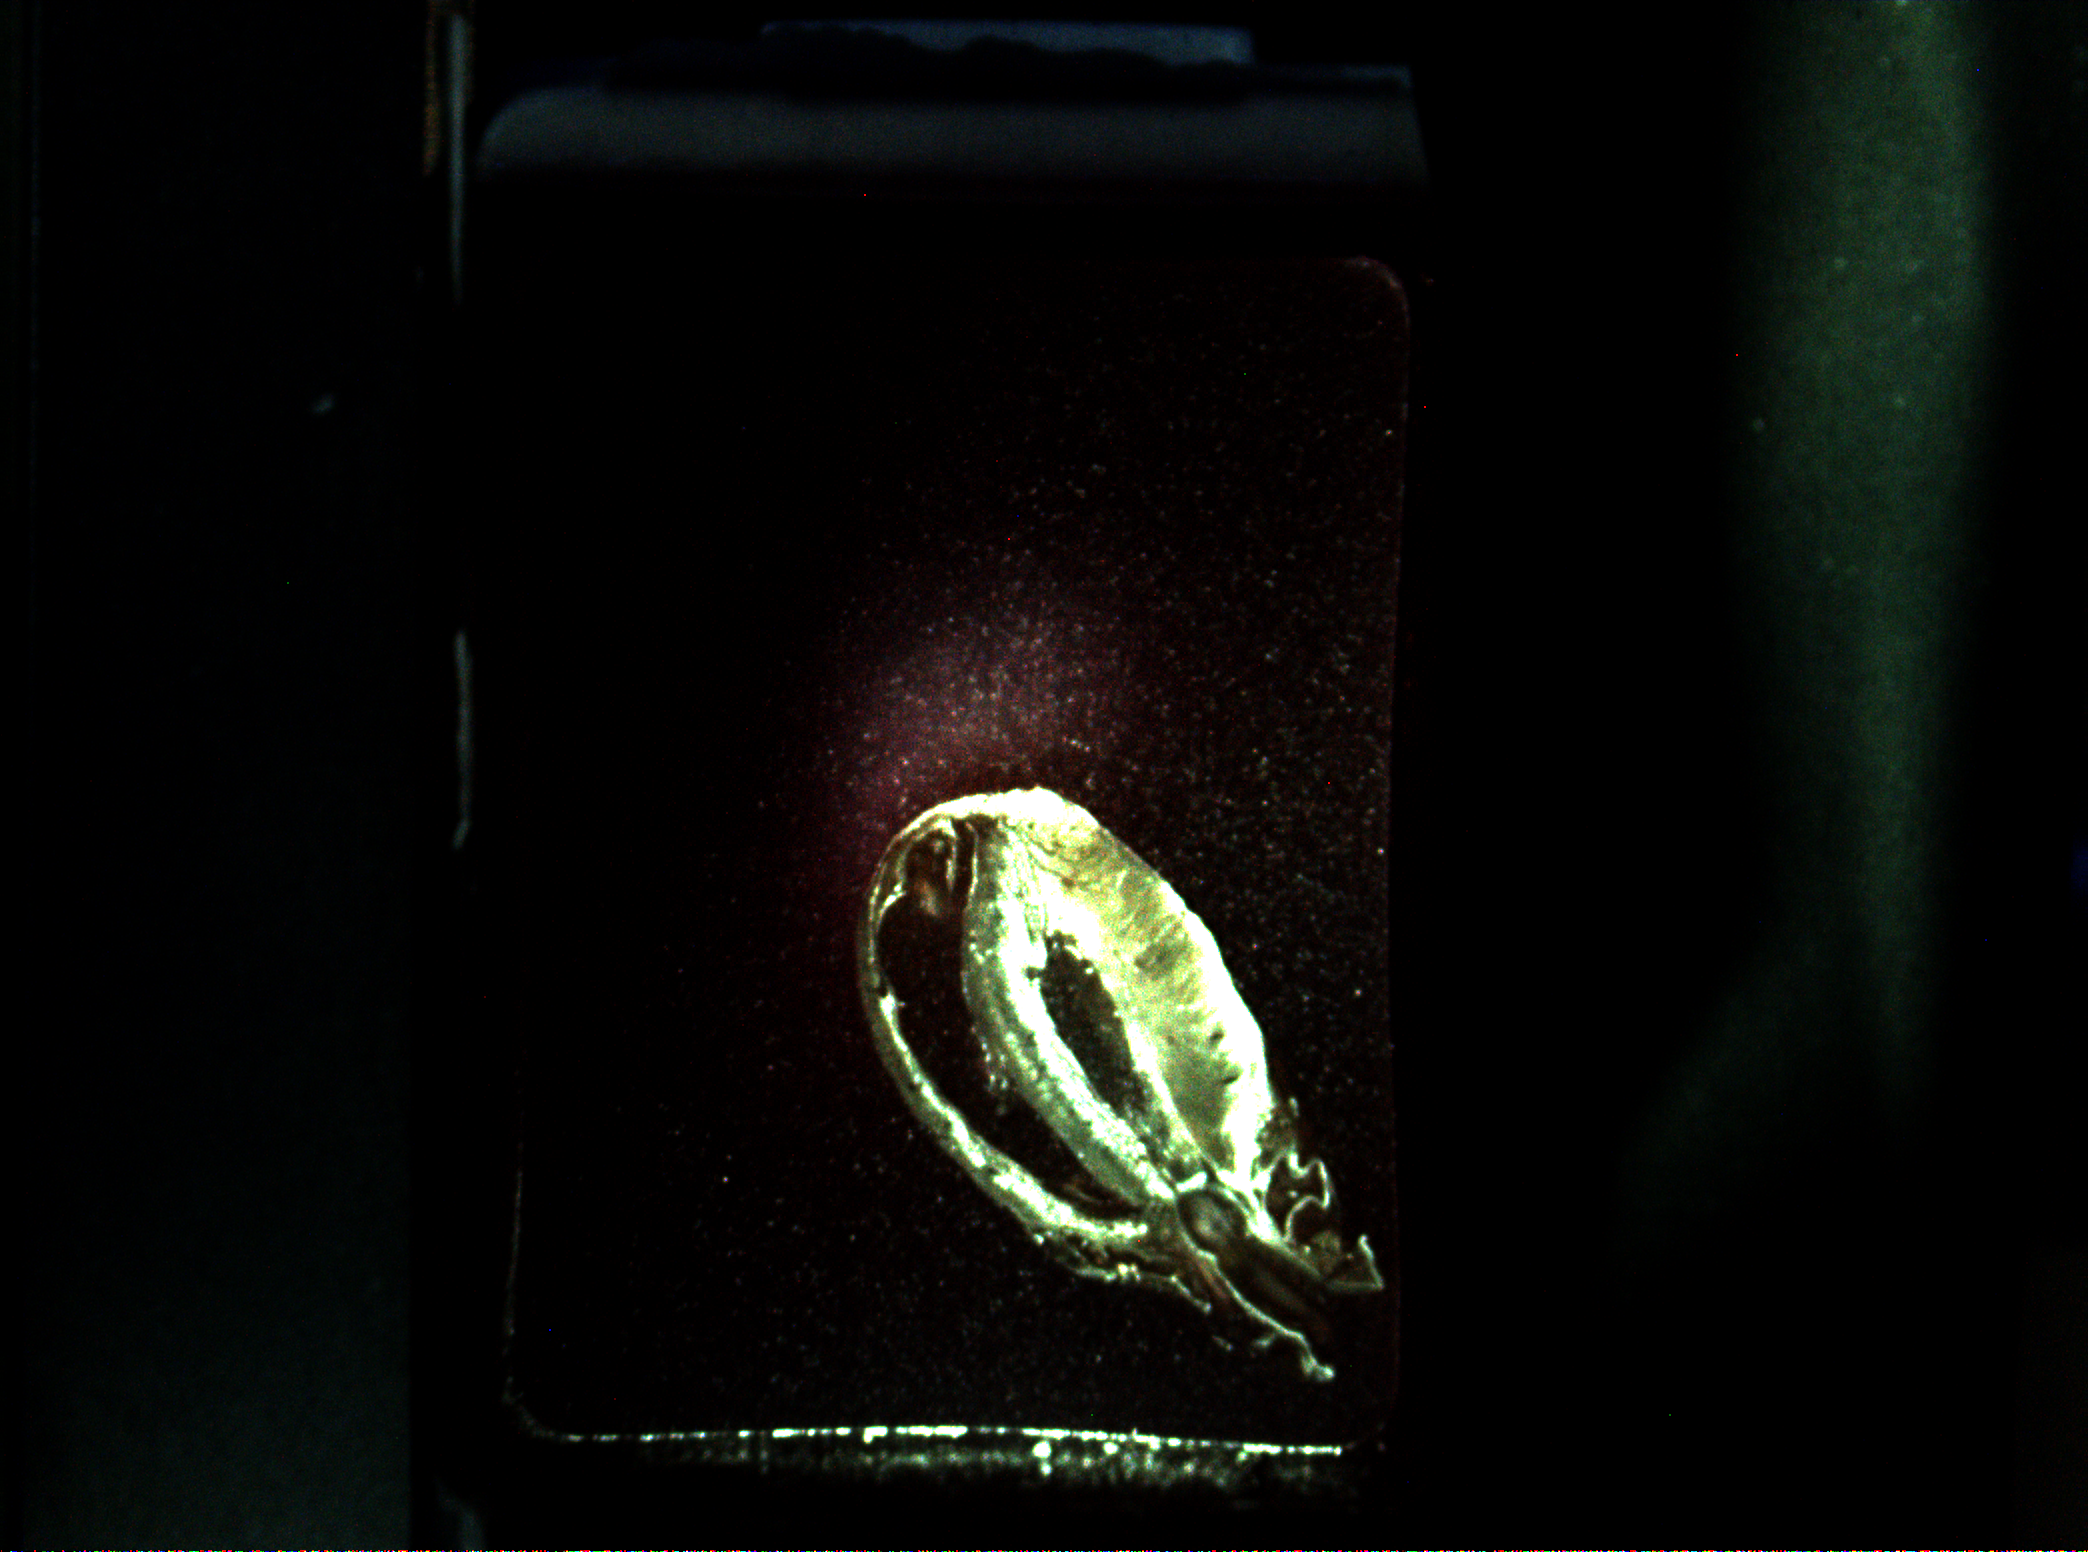
\includegraphics[width=0.8\pagewidth]{Ch6/Figs/LoRes_rgb_downsamples_1_0582}}
		  \subfigure[][]{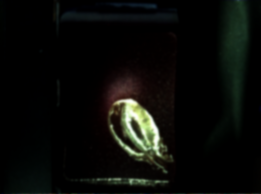
\includegraphics[width=0.8\pagewidth]{Ch6/Figs/LoRes_rgb_downsamples_8_0582}}
		  \caption{Block face images of slice 582 of Rat 28. The original image is shown in \textbf{(a)}, with \textbf{(b)} Gaussian smoothed and downsampled by a factor of 8 in each dimension.}
		  \label{fig:original_lores_images}
		\end{figure}
    
    \begin{figure}[htbp]
      \centering
      \subfigure[][]{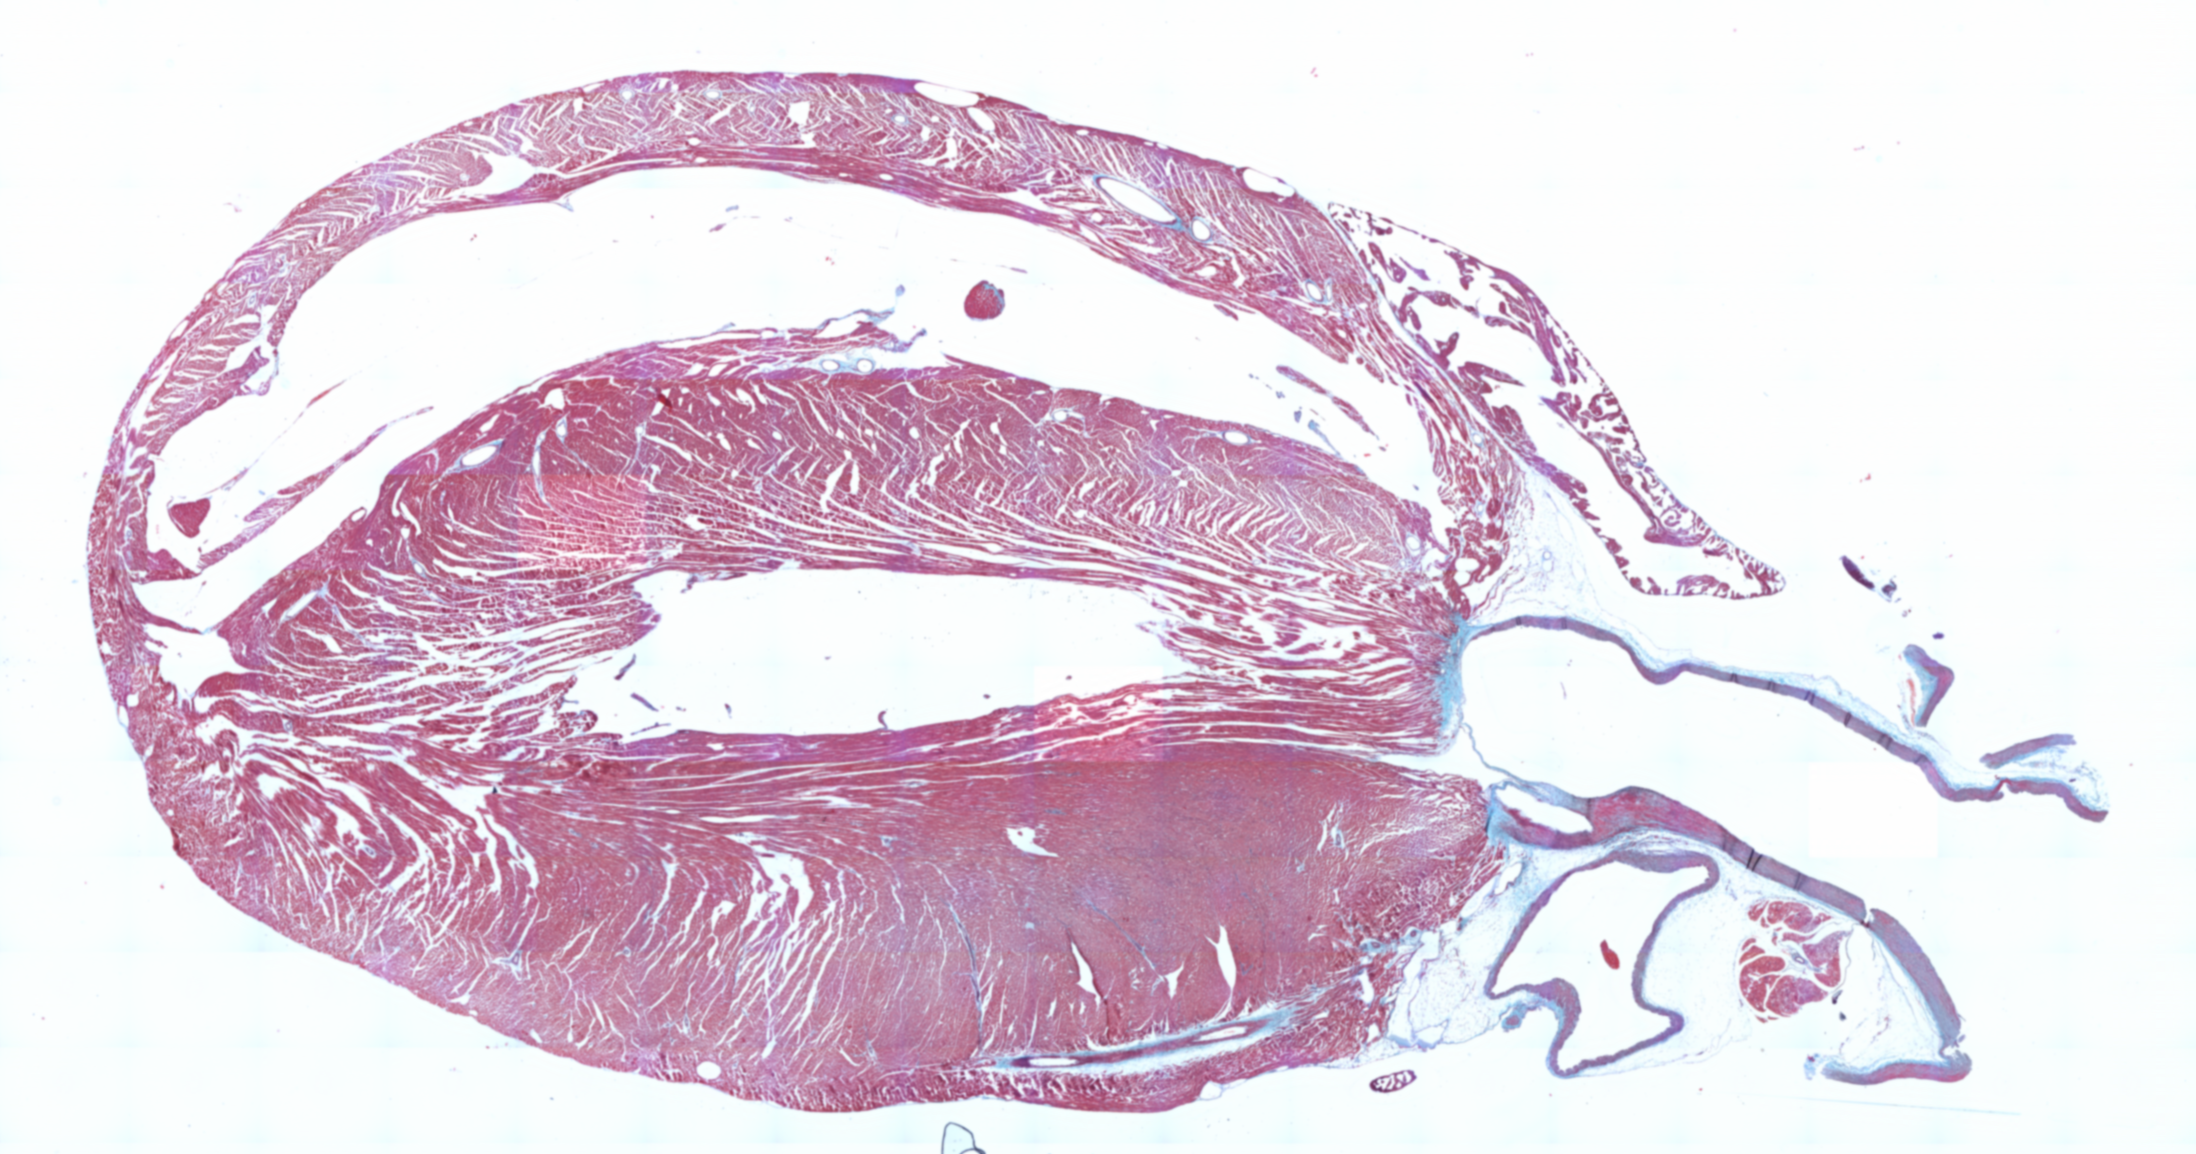
\includegraphics[width=0.8\pagewidth]{Ch6/Figs/HiRes_downsamples_8_0582}}
      \subfigure[][]{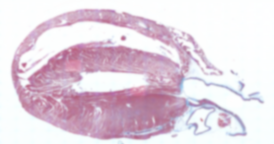
\includegraphics[width=0.8\pagewidth]{Ch6/Figs/HiRes_downsamples_64_0582}}
      \caption{Slice images of slice 582. \textbf{(a)} is Gaussian smoothed and downsampled by a factor of 8, and \textbf{(b)} by 64. The slice must be reflected and rotated in order to align with the block face image in Figure~\ref{fig:original_lores_images}.}
      \label{fig:original_hires_images}
    \end{figure}
	
  % subsection image_acquisition (end)

  \subsection{Image Curation} % (fold)
  \label{sub:image_curation}
    The images provided by Burton et al. yield unprecedented detail and quality. Although every possible step was taken during image acquisition, certain unavoidable experimental practicalities arose. A master subset of the images was selected, removing any slices with unacceptable damage such as that found in Figure~\ref{fig:damaged_slice}. Wherever a slice or group of slices was missing or removed, the acceptable adjacent slices were repeated symmetrically to fill the gap, in order to preserve the macroscopic geometry of the tissue. In the rare case where two images of the same slice existed, both slices were examined and the higher quality version was selected.
    
    \begin{figure}[htbp]
      \centering
      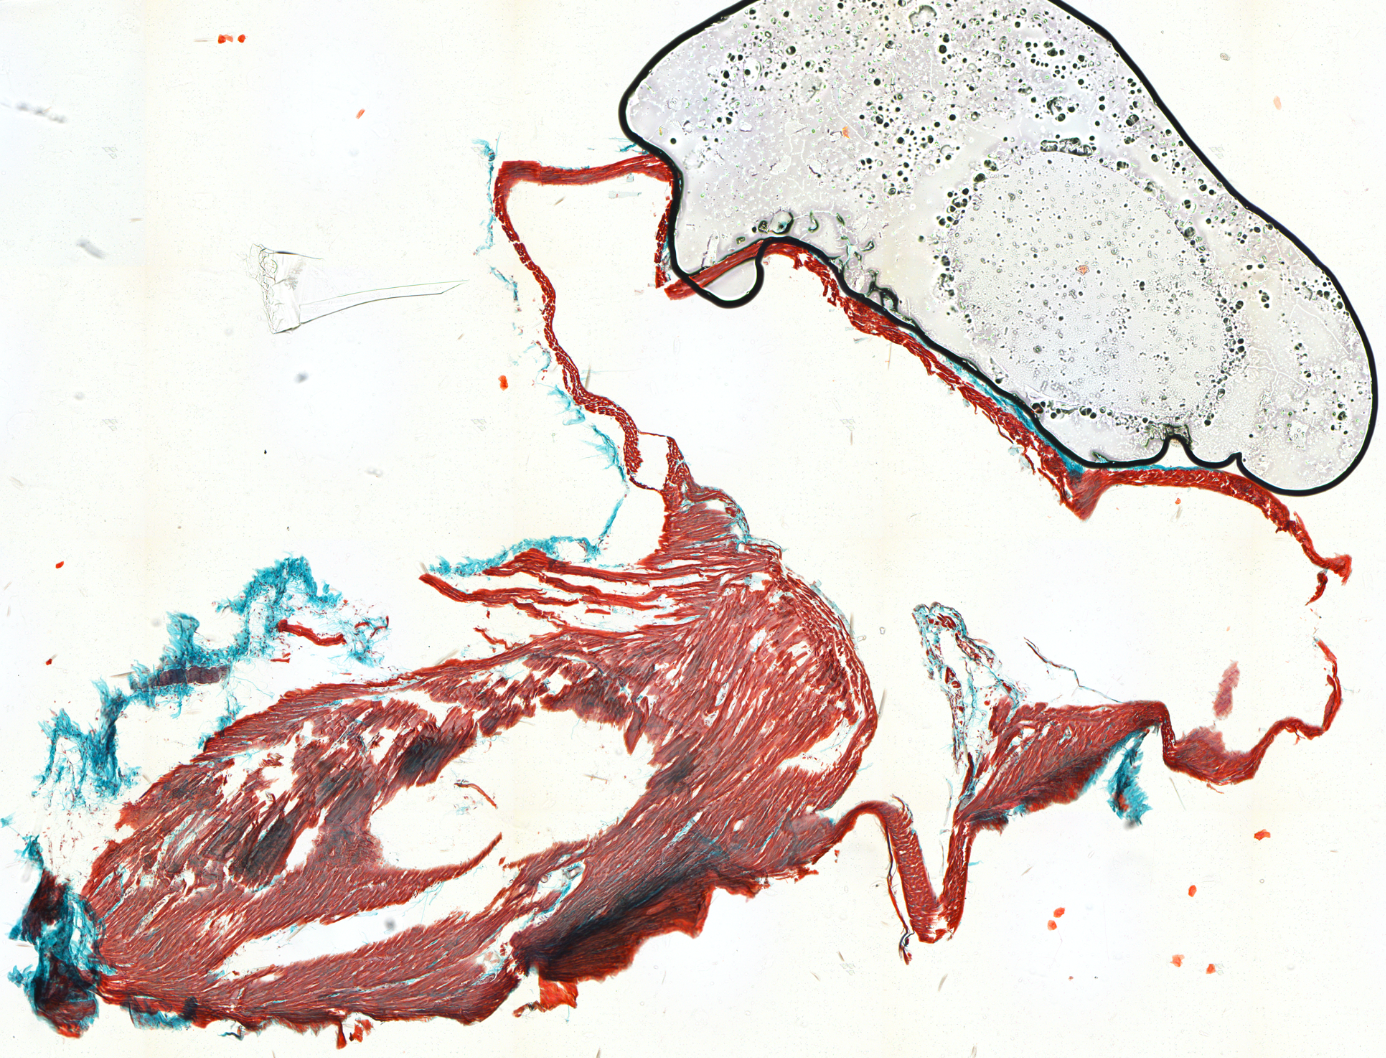
\includegraphics[width=.8\textwidth]{Ch6/Figs/damaged_slice}
      \caption{A damaged slice close to the left extremity of the heart. The tissue is severely damaged and folded in place. There is also a large bubble trapped between the two imaging slides.}
      \label{fig:damaged_slice}
    \end{figure}
    
  % subsection image_curation (end)
  
  \subsection{Image Preparation} % (fold)
  \label{sub:image_preparation}
  	The digital camera used to obtain the images created files with four channels: red, green, blue and alpha. Since transparency is meaningless in the context of a photograph, the alpha channel was uniformly black. Unfortunately, the implementation of the RGBA BMP reader in ITK labels the channels incorrectly. To correct for this, channels were explicitly permuted and the redundant alpha channel removed.
  
    On occasion, part way through image acquisition, the block face camera would be moved relative to the surface of the wax block. All images acquired from then on had to be translated and rotated to compensate for this movement. At each perturbation, the two slices between which the camera had moved were registered in order to calculate the corrective transform, which was then applied to all subsequent slices. Figure~\ref{fig:LoRes_cross_sections} depicts the results of these corrections, and the isosurface of the corrected segmented volume are shown from 6 sides in Figures~\labelcref{fig:LoRes_positive_x,fig:LoRes_negative_x,fig:LoRes_positive_y,fig:LoRes_negative_y,fig:LoRes_positive_z,fig:LoRes_negative_z}. The isosurface was generated from a threshold segmentation of the intensity magnitude of the volume. A dense cloud of wax bubbles and other small artefacts obscured the main surface of the heart, and so a binary shape opening filter was applied to remove all but the largest connected region from the segmentation before the contour was extracted.
    
    % lores cross sections
    \begin{sidewaysfigure}[htbp]
      \centering
      \subfigure[][]{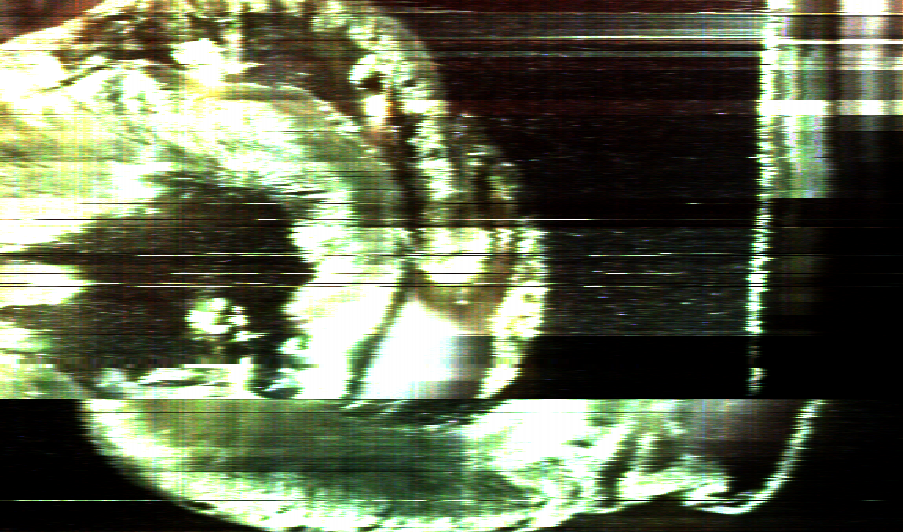
\includegraphics[height=0.31\textheight]{Ch6/Figs/LoRes_without_adjustments_0_235}}
      \subfigure[][]{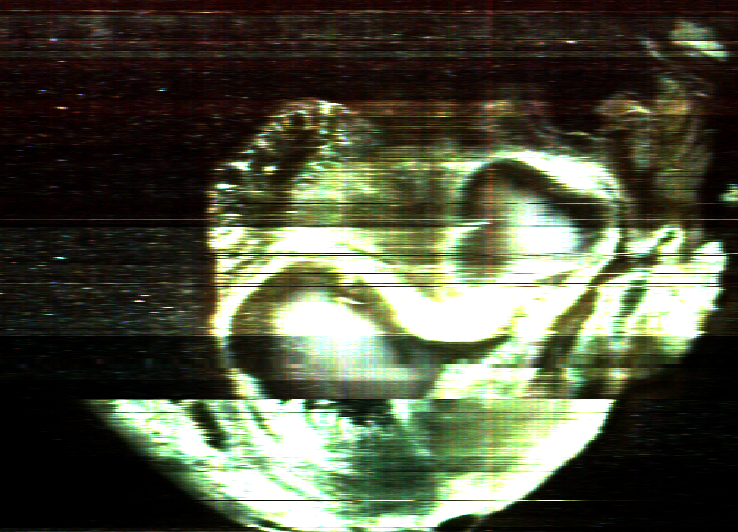
\includegraphics[height=0.31\textheight]{Ch6/Figs/LoRes_without_adjustments_1_287}}
      \subfigure[][]{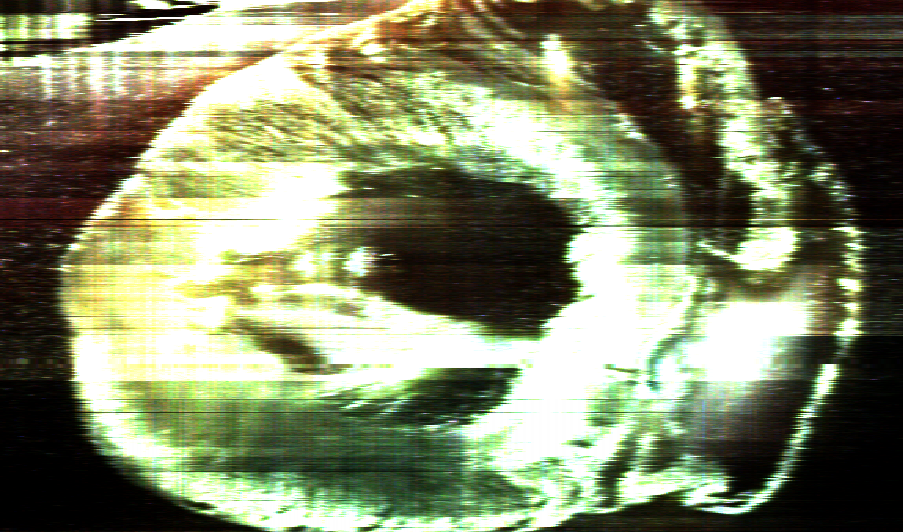
\includegraphics[height=0.31\textheight]{Ch6/Figs/LoRes_0_235}\label{subfig:LoRes_adjusted_long_cross_section}}
      \subfigure[][]{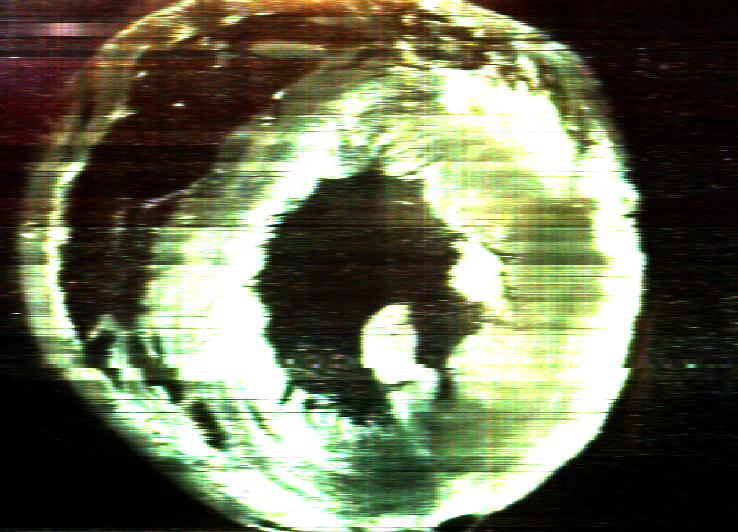
\includegraphics[height=0.31\textheight]{Ch6/Figs/LoRes_1_287}}
      \caption{Central cross-sections of the cropped block-face volume. \textbf{(a)} and \textbf{(b)} show the volume before adjustment, where a large camera displacement is apparent approximately a quarter of the way from the bottom of the image. Several thin stripes are visible further up, where the occasional single image has been displaced. The volume is fully aligned in \textbf{(c)} and \textbf{(d)}, with striations visible due to discrete changes in the positioning and intensity of illumination. These changes will propagate to the final registration result.}
      \label{fig:LoRes_cross_sections}
    \end{sidewaysfigure}
    
    % lores contours
    \begin{sidewaysfigure}[htbp]
      \centering
      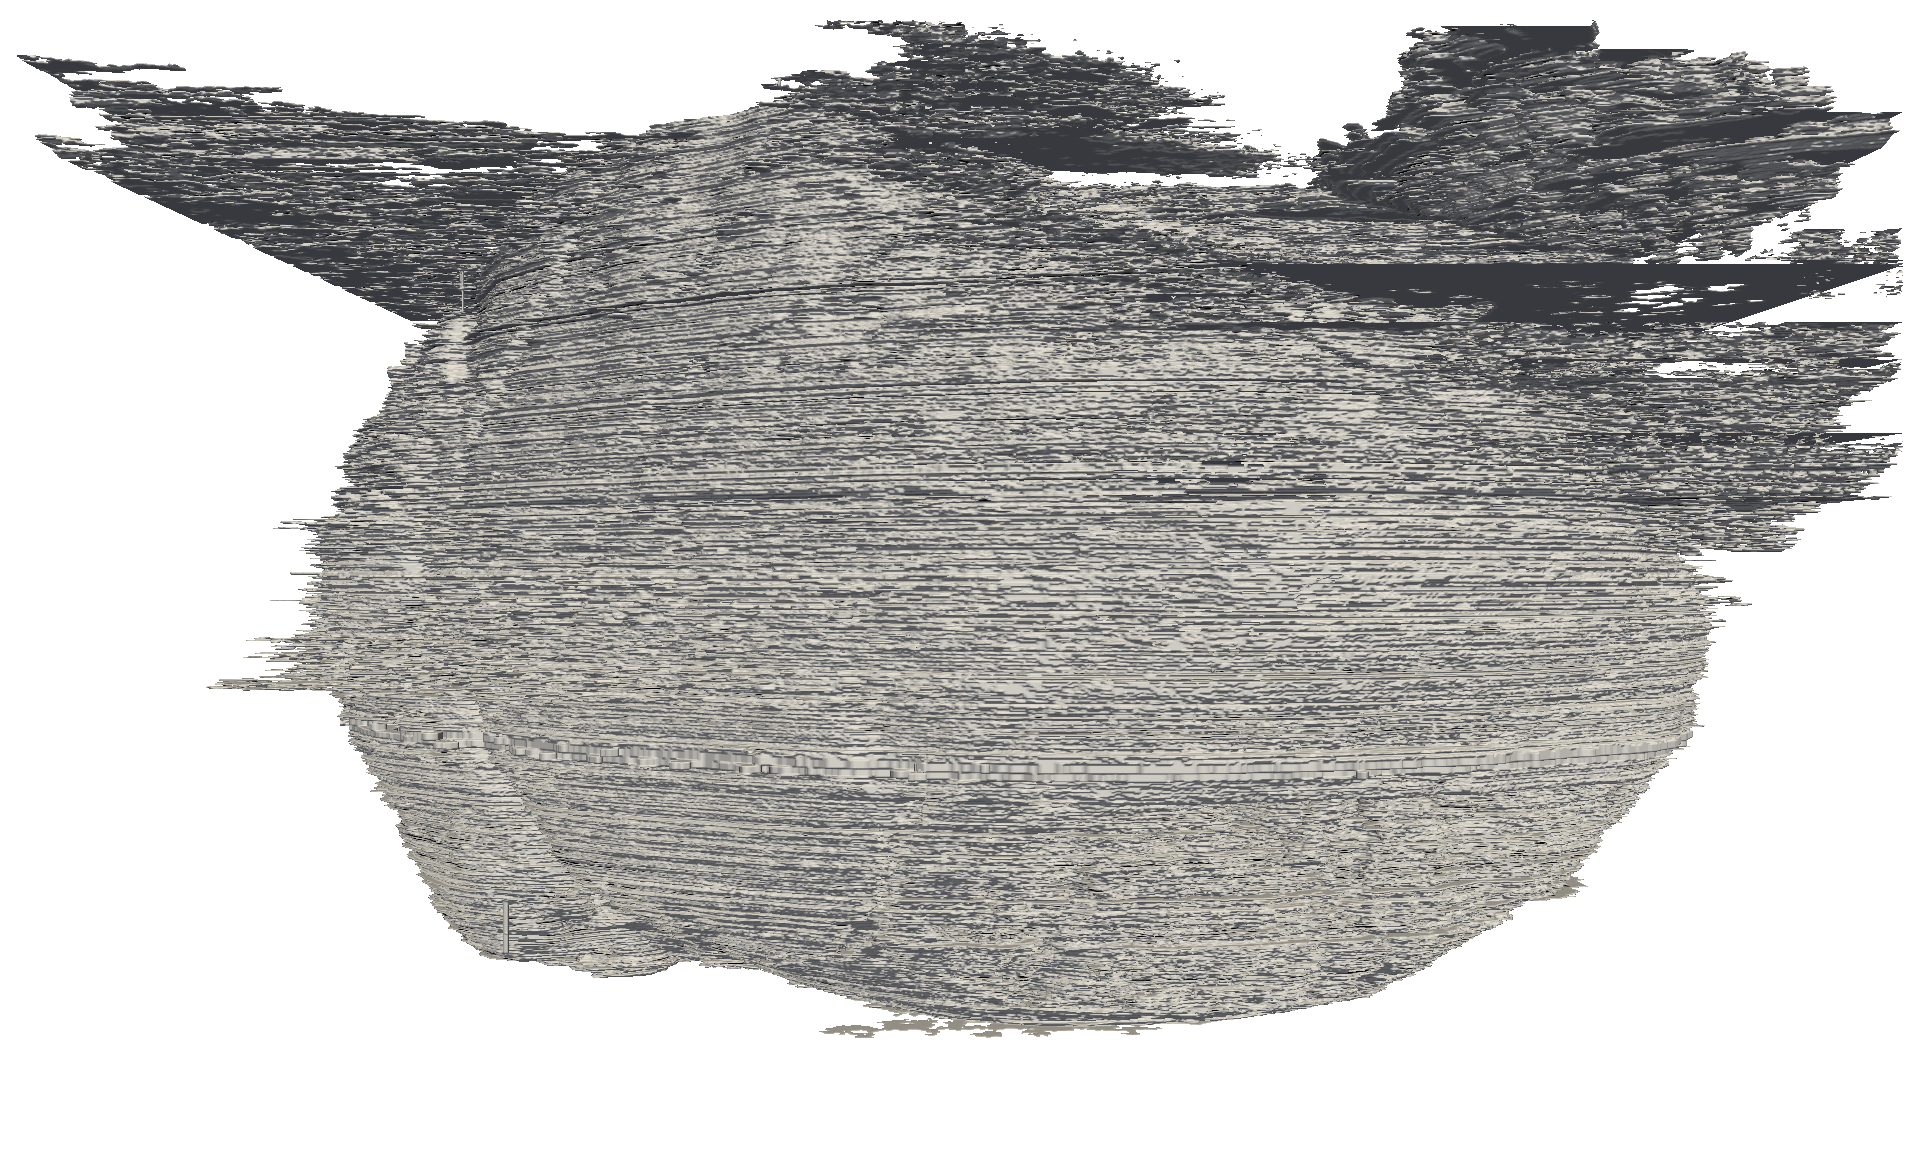
\includegraphics[width=\textheight]{Ch6/Figs/Rat28/contours/LoRes_positive_x}
      \caption{A contour of the adjusted block face volume, viewed along the positive x direction. The round surface of the heart apex is clearly visible to the right. Oddly shaped protrusions in the top third of slices are due to gradually brightening reflection from the suface of the wax.}
      \label{fig:LoRes_positive_x}
    \end{sidewaysfigure}
    
    \begin{sidewaysfigure}[htbp]
      \centering
      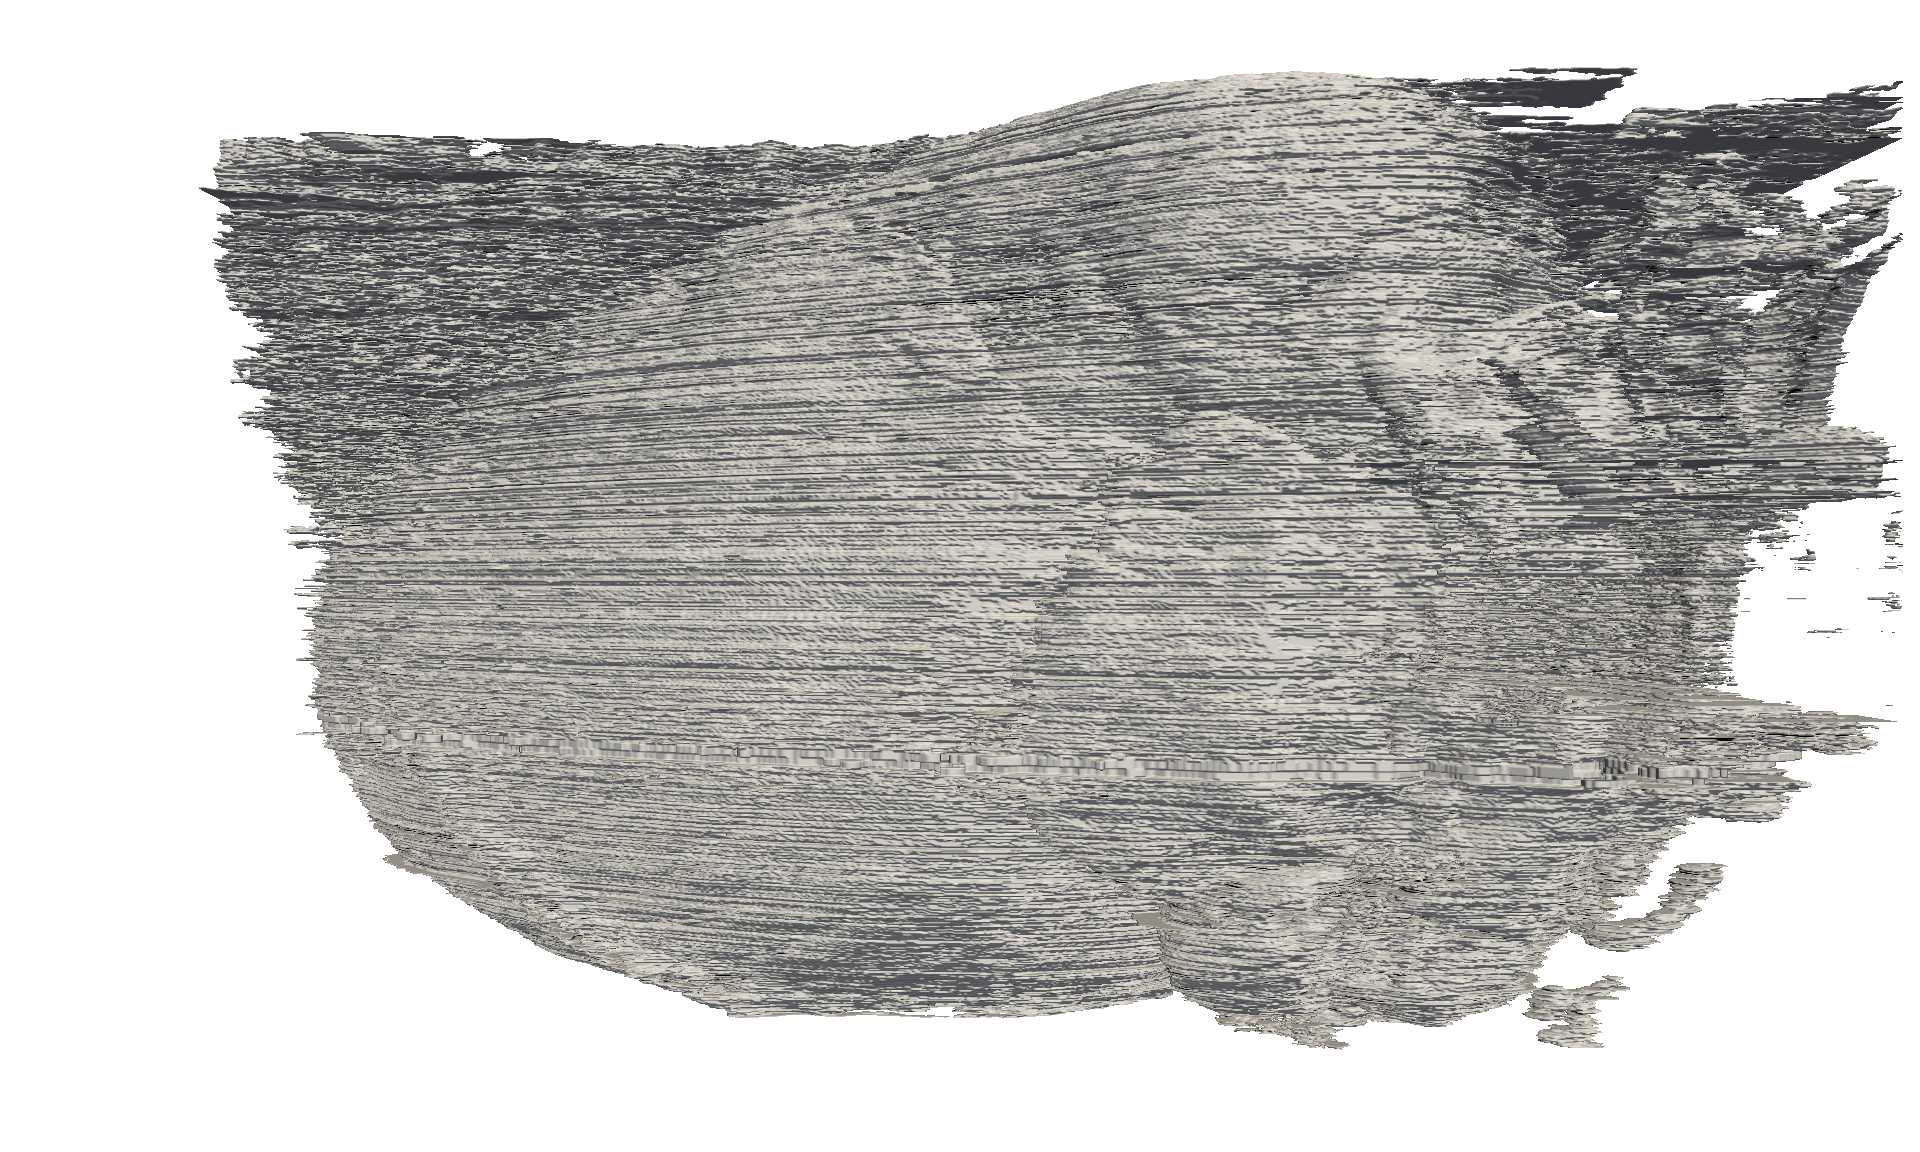
\includegraphics[width=\textheight]{Ch6/Figs/Rat28/contours/LoRes_negative_x}
      \caption{The block face contour viewed along the negative x direction. The more complex surface of the valve and vascular machinery at the base of the heart is visible to the right.}
      \label{fig:LoRes_negative_x}
    \end{sidewaysfigure}
    
    \begin{sidewaysfigure}[htbp]
      \centering
      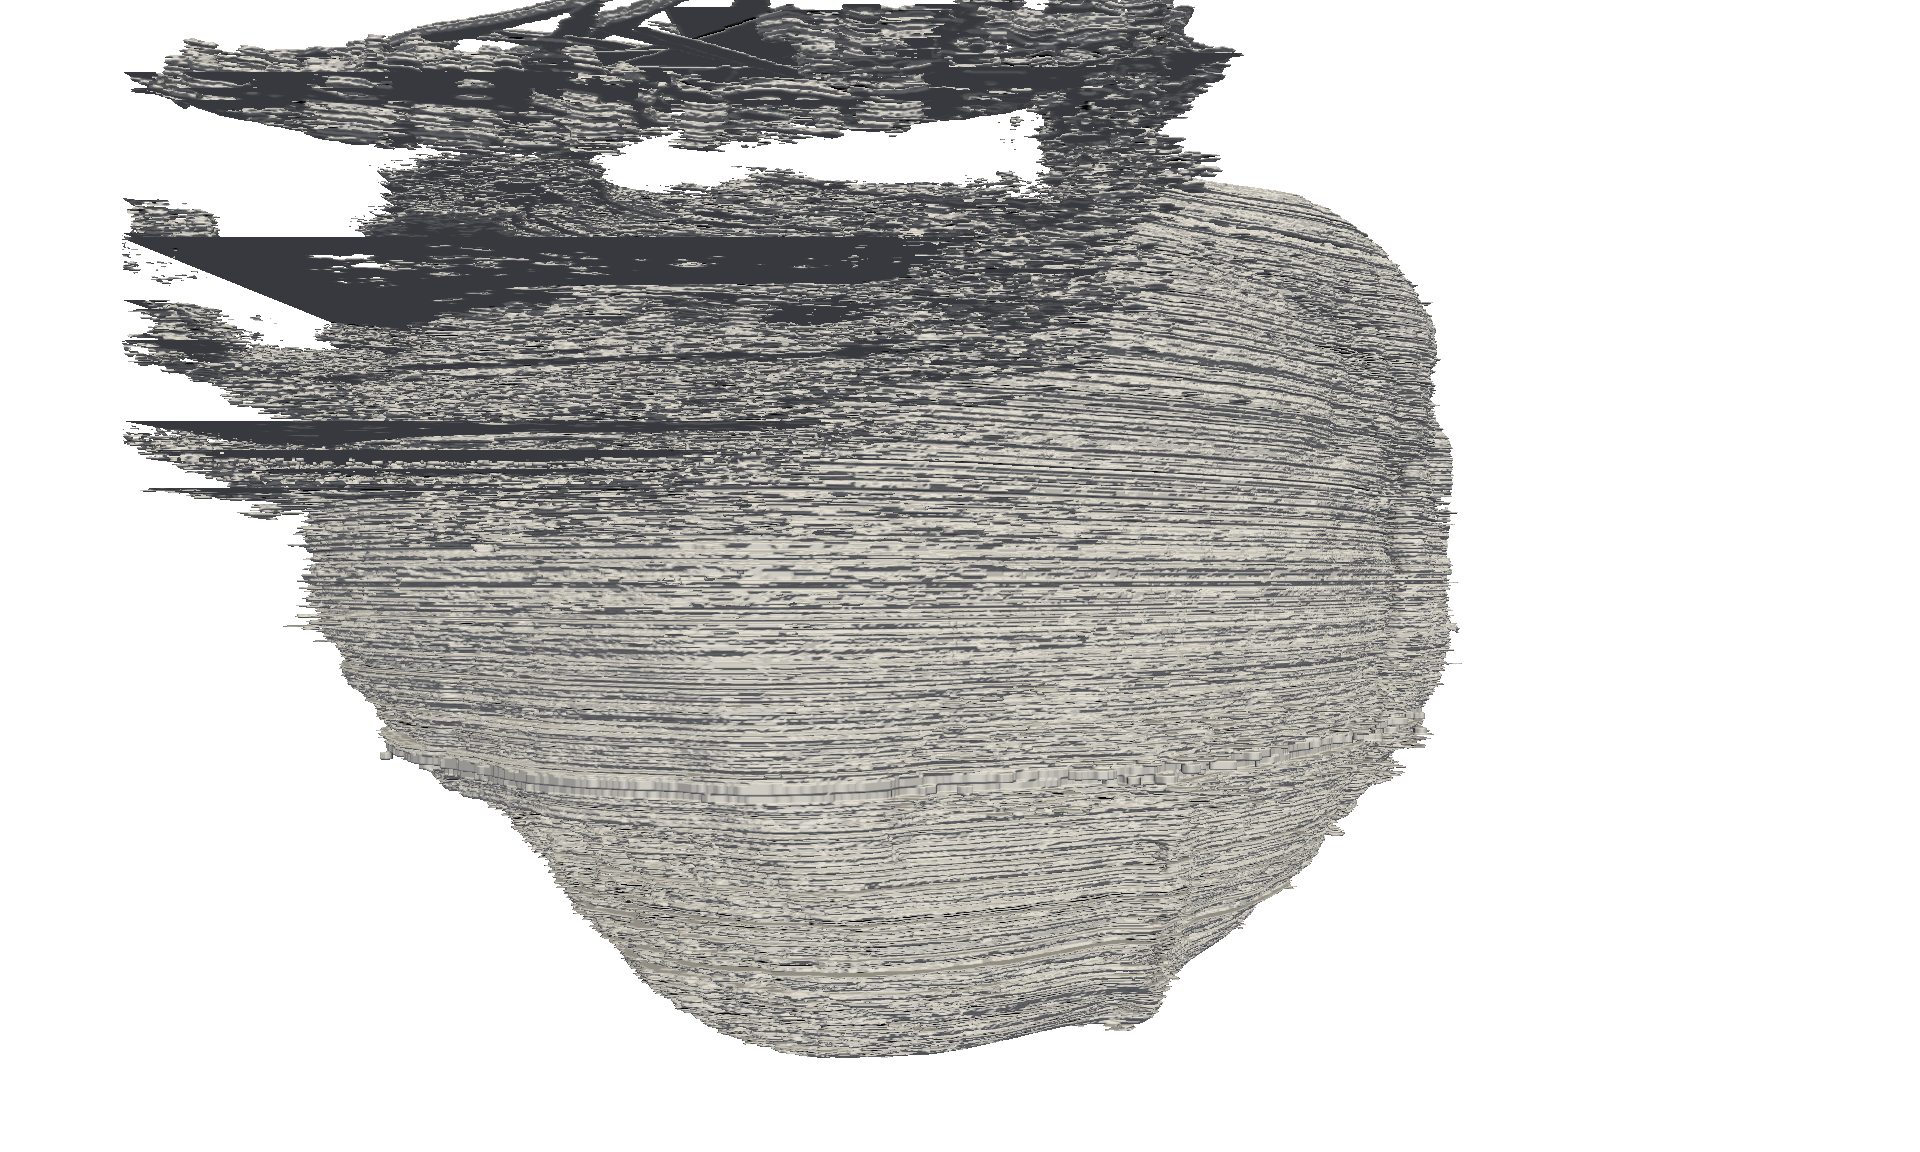
\includegraphics[width=\textheight]{Ch6/Figs/Rat28/contours/LoRes_positive_y}
      \caption{The block face contour viewed along the positive y direction. The bulge of an epicardial vessel at the bottom right hand side is clearly visible (it is also faintly visible towards the bottom left of Figure~\ref{fig:LoRes_negative_x}). The discrete change in illumination from Figure~\ref{subfig:LoRes_adjusted_long_cross_section} manifests as an apparent increase in surface size approximately a third of the height from the bottom.}
      \label{fig:LoRes_positive_y}
    \end{sidewaysfigure}
    
    \begin{sidewaysfigure}[htbp]
      \centering
      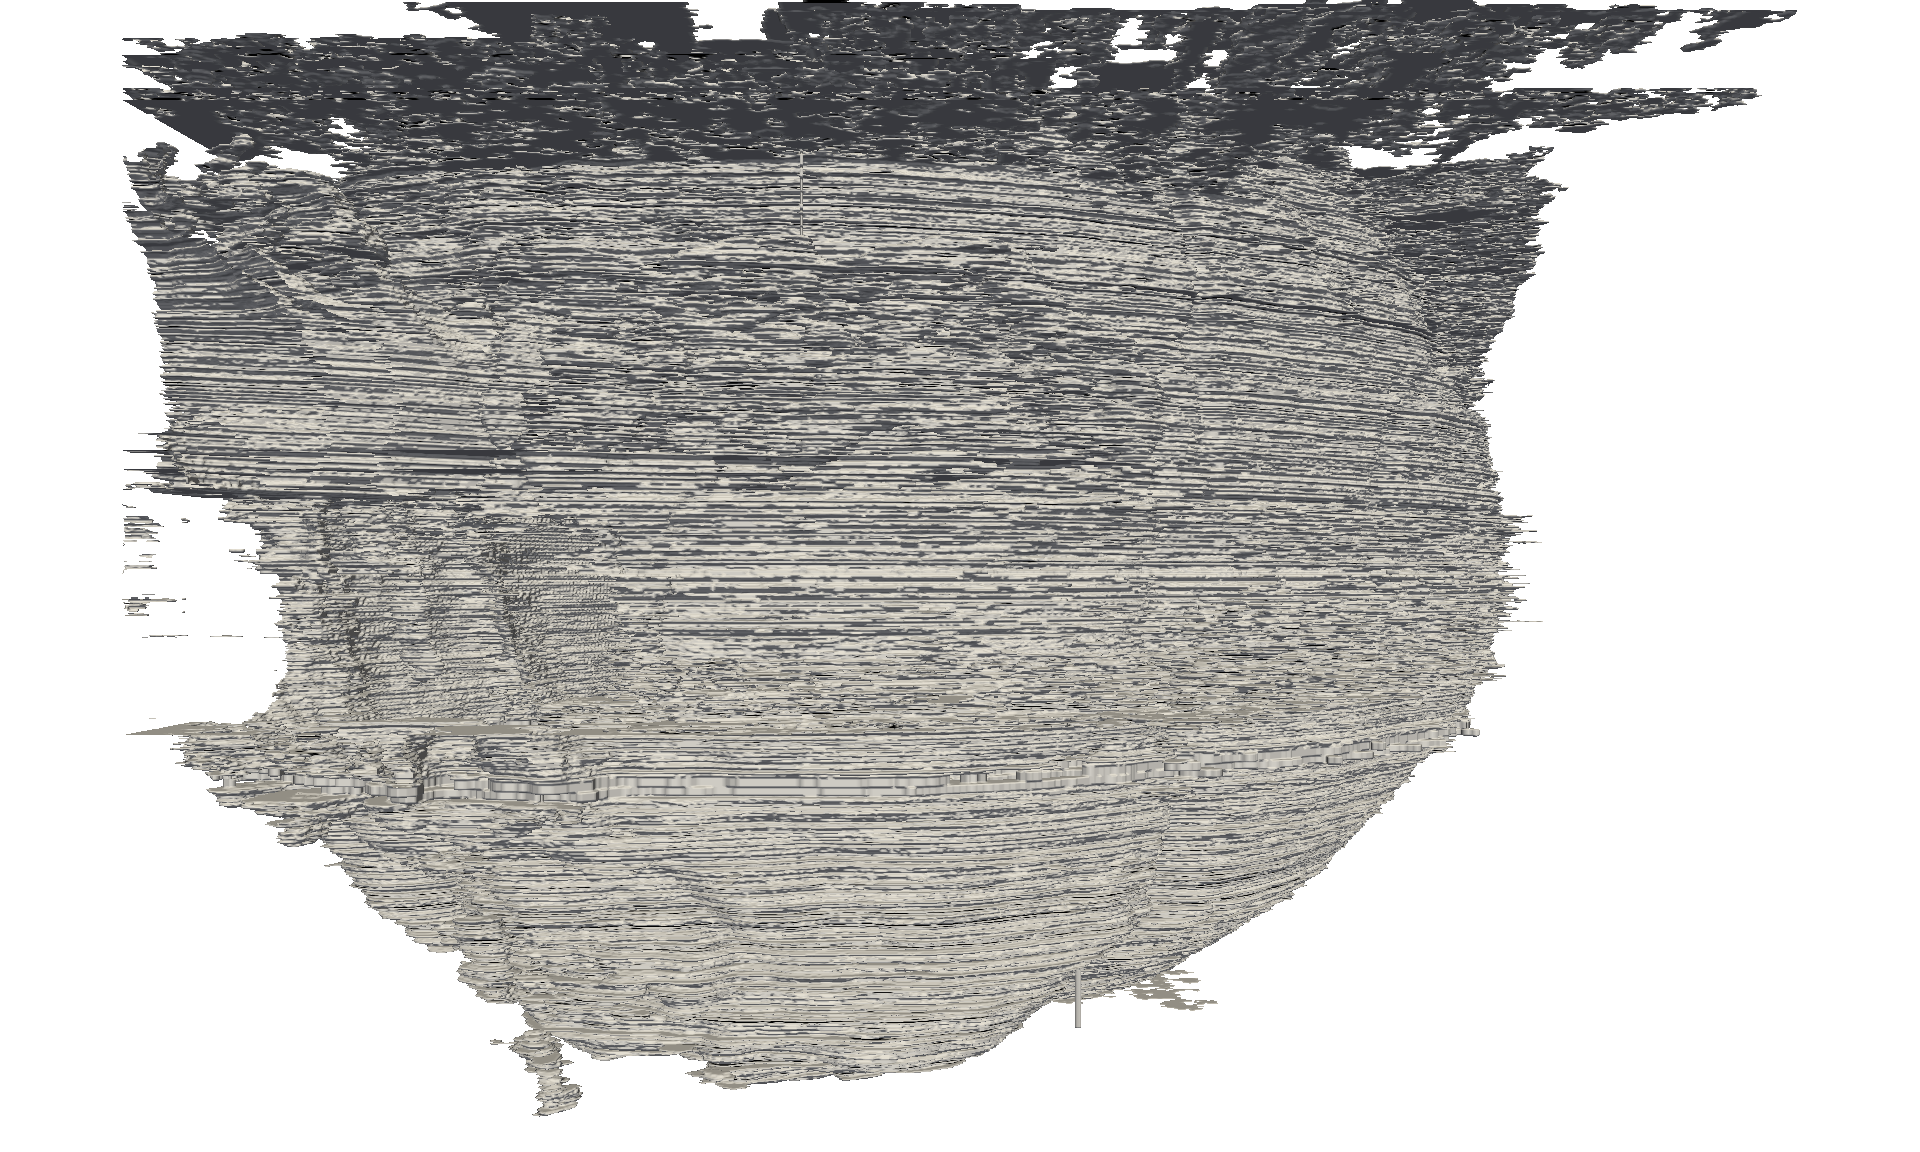
\includegraphics[width=\textheight]{Ch6/Figs/Rat28/contours/LoRes_negative_y}
      \caption{The block face contour viewed along the negative y direction.}
      \label{fig:LoRes_negative_y}
    \end{sidewaysfigure}
    
    \begin{sidewaysfigure}[htbp]
      \centering
      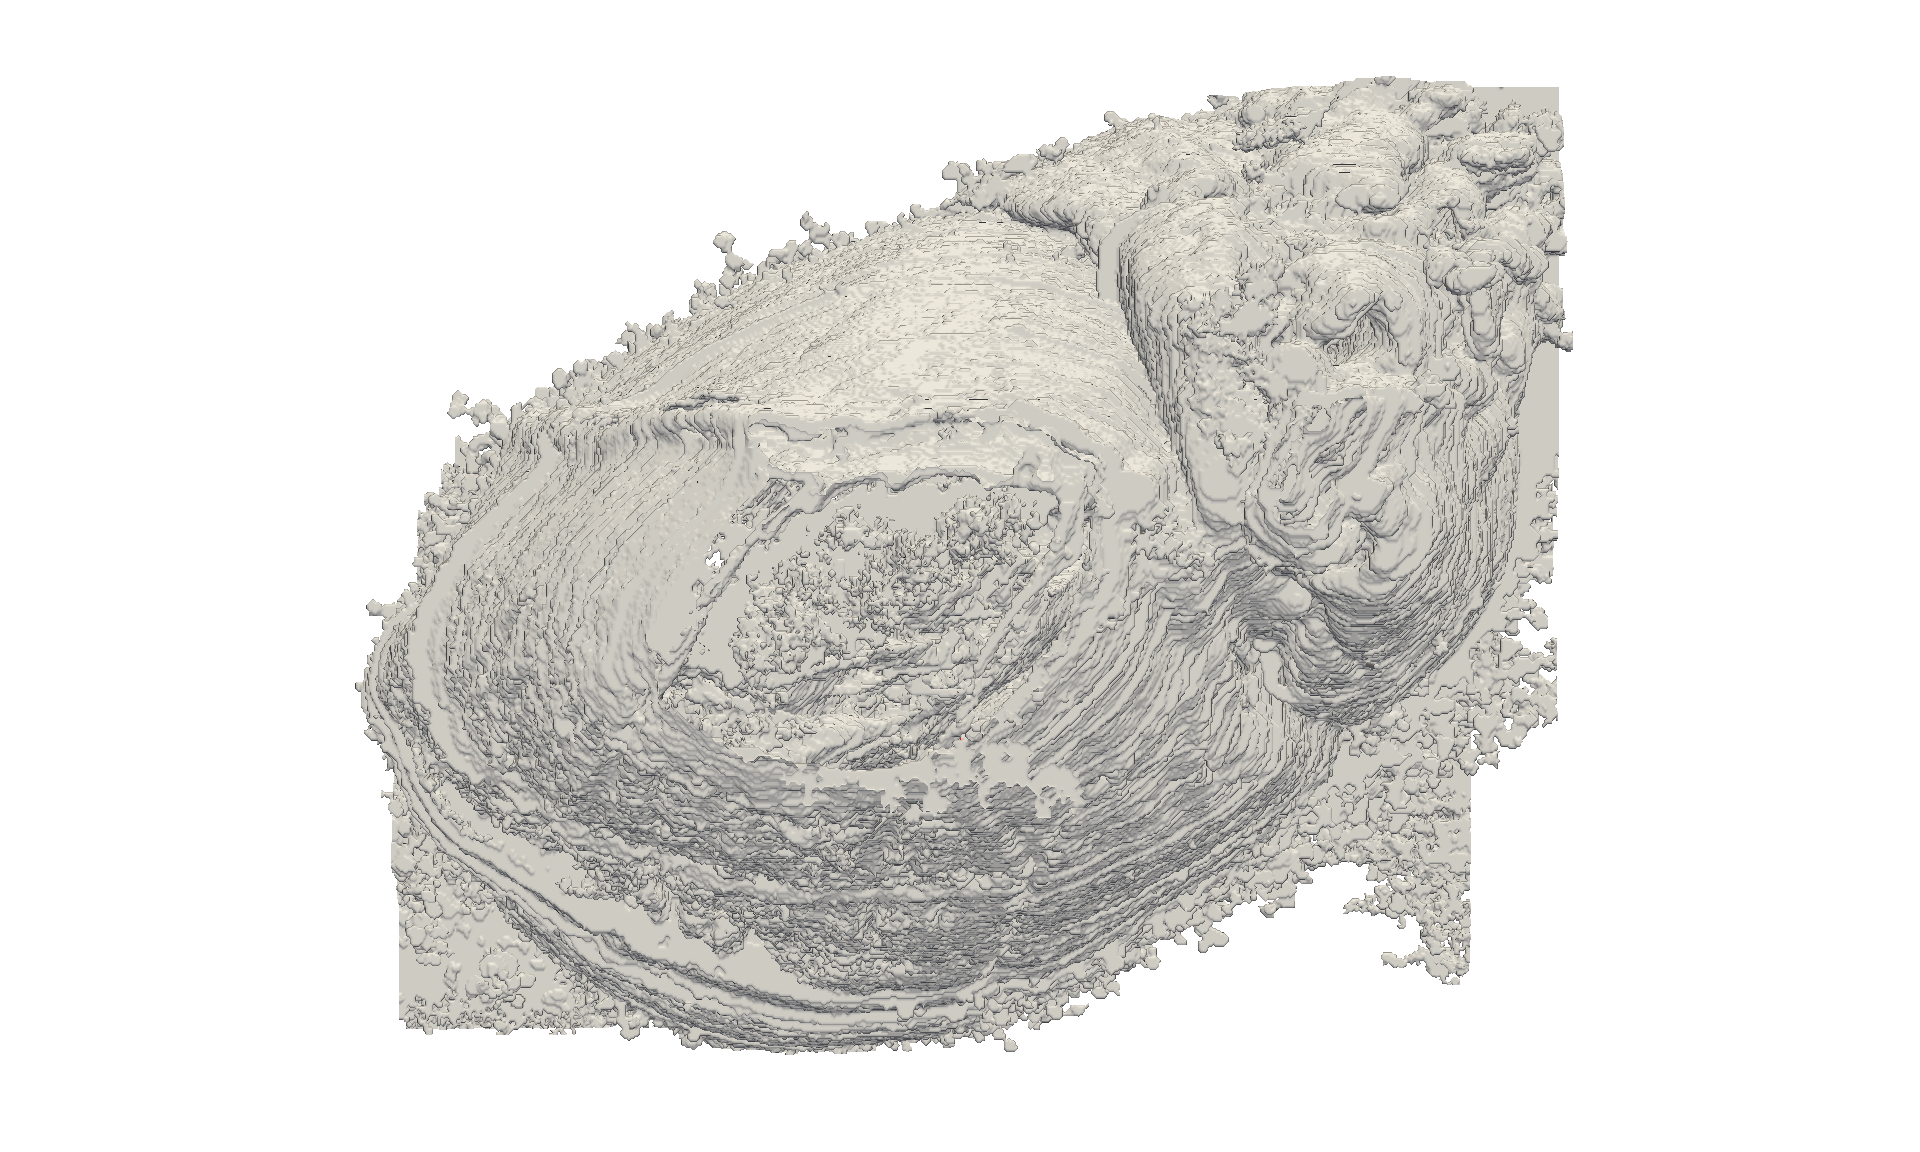
\includegraphics[width=\textheight]{Ch6/Figs/Rat28/contours/LoRes_positive_z}
      \caption{The block face contour viewed along the positive z direction. The detail and composition of the images is clearly visible from this angle. Note the protruding epicardial vessel in the top left. The surface of the first third of slices near the bottom left looks eroded, in a region where the threshold intensity values have failed to pick up the tissue boundary faithfully.}
      \label{fig:LoRes_positive_z}
    \end{sidewaysfigure}
    
    \begin{sidewaysfigure}[htbp]
      \centering
      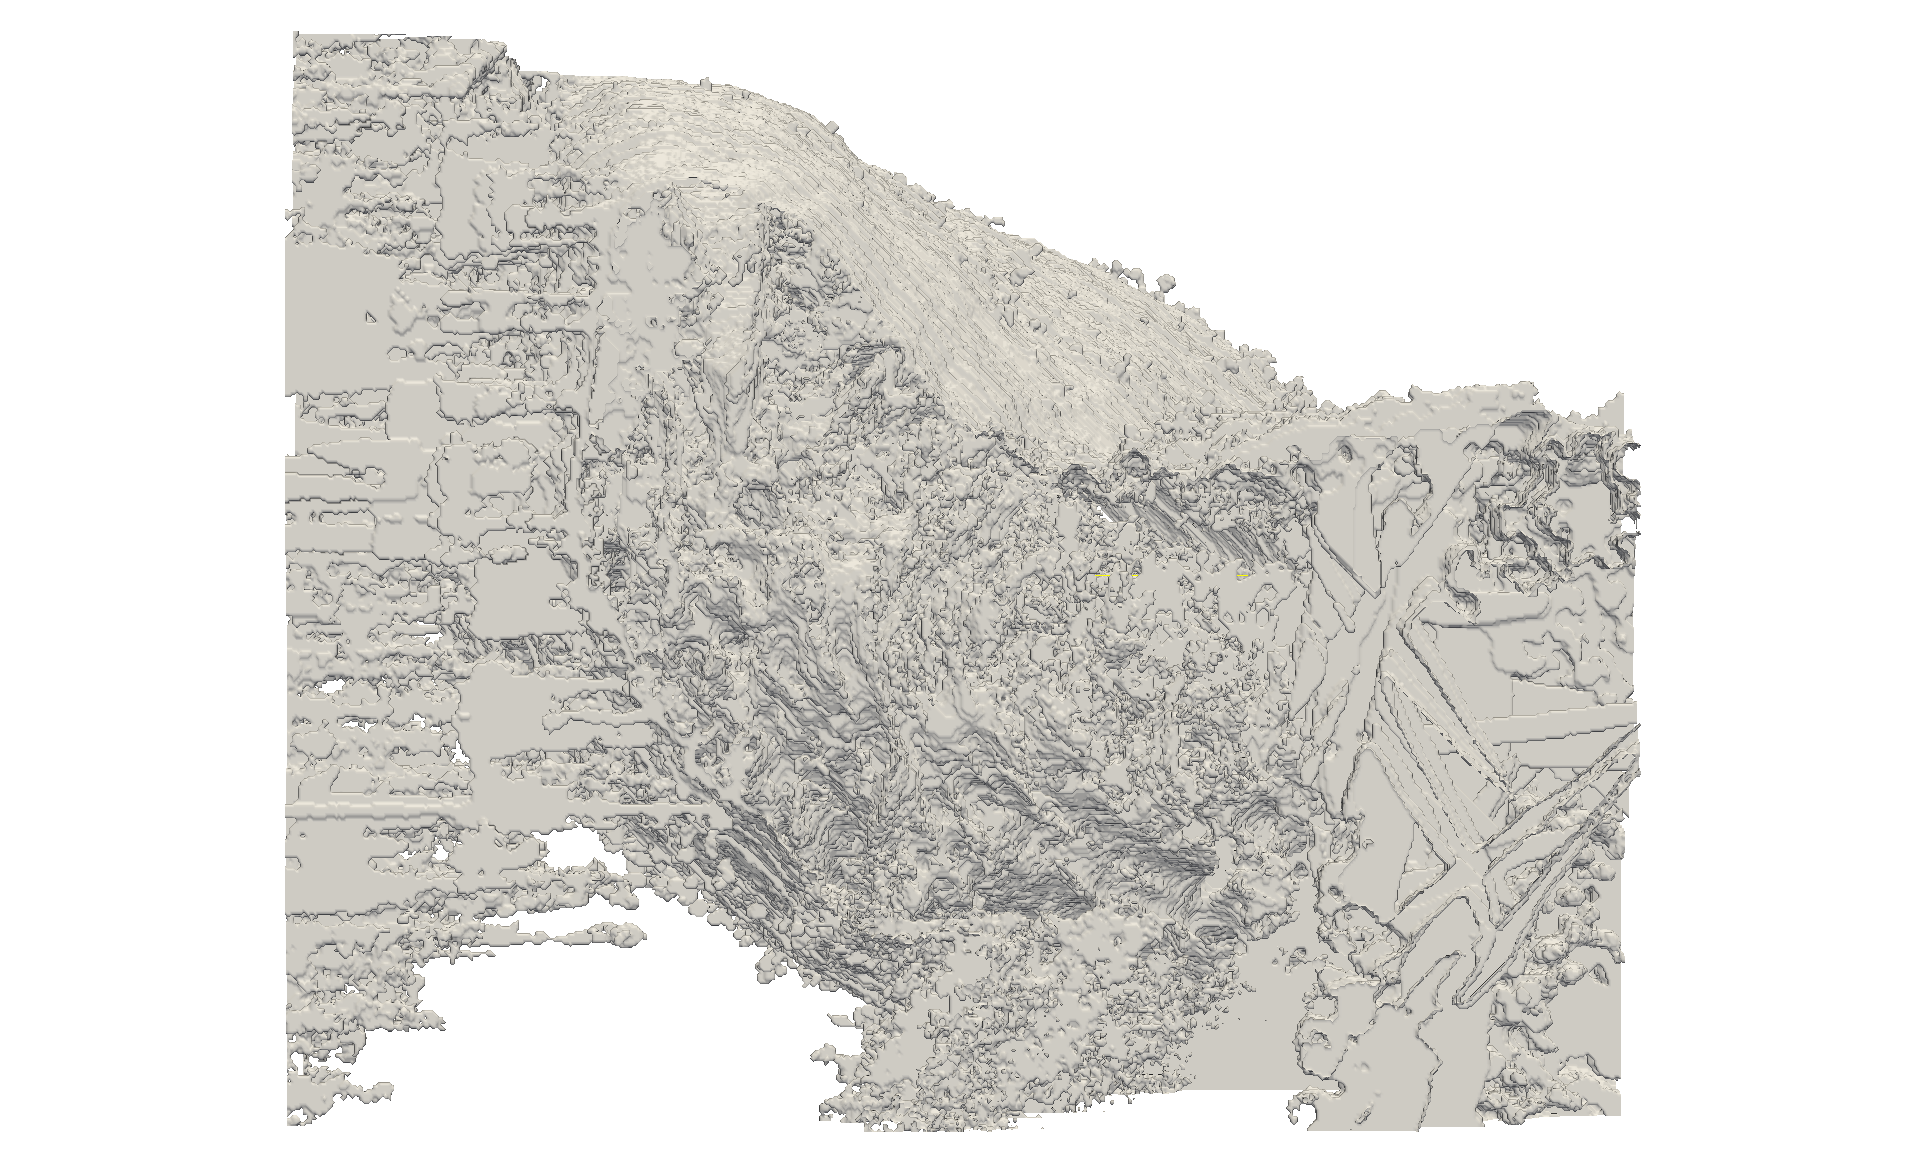
\includegraphics[width=\textheight]{Ch6/Figs/Rat28/contours/LoRes_negative_z}
      \caption{The block face contour viewed along the negative z direction. Bright reflection obscures much of the tissue surface from this angle, and the accurate registration of these top slices will prove impossible.}
      \label{fig:LoRes_negative_z}
    \end{sidewaysfigure}
    
	As is evident from Figures~\labelcref{fig:original_lores_images,fig:original_hires_images} for one slice, the vast majority of slices had been flipped over between sectioning from the block surface and being photographed. Slice images were therefore reflected across one axis in order to restore geometric parity with the associated block face image.
	
	 Several sets of downsamples of varying factors were generated, the lowest of which were used for debugging and testing, working up in detail, size and computational expense as the techniques were perfected. Before downsampling, a Gaussian smoothing was applied in each case, with sigma equal to the new larger pixel spacing. In this way, all original pixels in the region of a large downsampled pixel contribute to its final value, and aliasing noise problems associated with frthe Nyquist frequency are avoided. This results in a smoother and more accurate cost function. Figures~\labelcref{fig:original_lores_images,fig:original_hires_images} juxtapose the full images with various levels of downsampling.
	 
	 When registering two images, it is important that they are of comparable resolution, in order to minimise processing time and to ensure the smoothest possible cost function. In Figure~\ref{fig:downsample_zooms}, the effects of the downsampling can be seen more clearly. Individual cell nuclei are resolved at the highest resolution of slice image, but the maximum resolution block face images are of much lower detail. Clearly, the original slice images, with 1.1$\mu$m pixel spacings, are needlessly detailed compared to their block face counterparts, with a mere 26.6$\mu$m. As is discussed in Section~\ref{ssub:multiresolution_registration}, it is therefore appropriate to register slice images at a factor of 8 times more downsampled than the block face images.
    
	%  Lo/HiRes zooms
    \begin{sidewaysfigure}[htbp]
      \centering
      \subfigure[][]{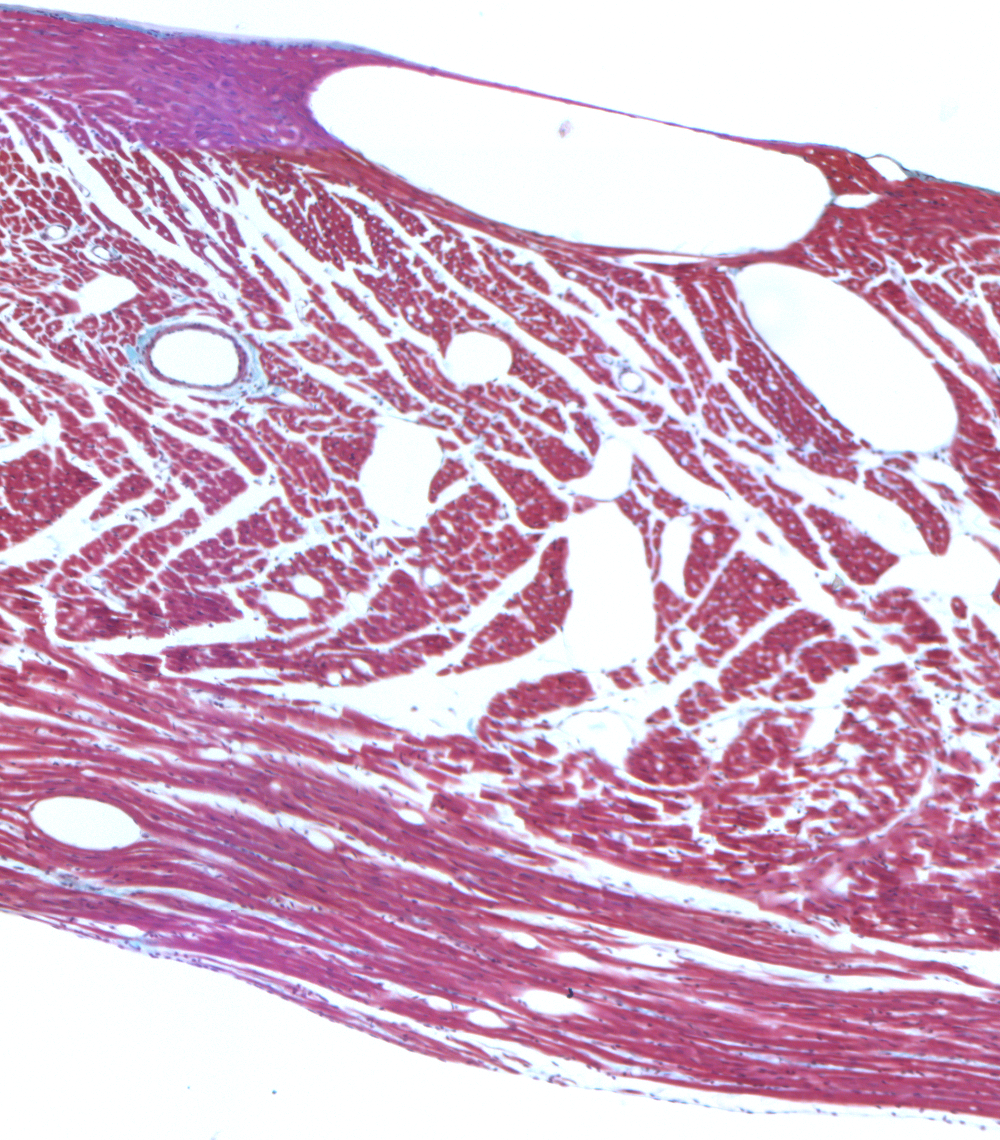
\includegraphics[width=0.39\pagewidth]{Ch6/Figs/HiRes_downsamples_1_0582_zoom}}
      \subfigure[][]{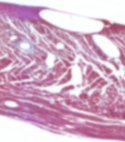
\includegraphics[width=0.39\pagewidth]{Ch6/Figs/HiRes_downsamples_8_0582_zoom}}
      \subfigure[][]{
\includegraphics[width=0.39\pagewidth]{Ch6/Figs/HiRes_downsamples_64_0582_zoom}}
      \subfigure[][]{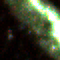
\includegraphics[width=0.39\pagewidth]{Ch6/Figs/LoRes_rgb_downsamples_1_0582_zoom}}
      \subfigure[][]{
\includegraphics[width=0.39\pagewidth]{Ch6/Figs/LoRes_rgb_downsamples_8_0582_zoom}}
      \caption{An epicardial vessel in slice 582 of Rat 28, in both the slice and the block face images. \textbf{(a)}, \textbf{(b)} and \textbf{(c)} show the slice original, 8x and 64x downsampled, while \textbf{(d)} and \textbf{(e)} show the block face original and 8x downsampled. The fibres parallel to the internal wall at the bottom of \textbf{(a)} are angled such that they reflect the illumination strongly at the top right of \textbf{(d)}, and are in much sharper contrast to the black wax than the rest of the tissue. Indeed, they are in much sharper contrast to the other tissue than the other tissue is to the non-tissue.}
      \label{fig:downsample_zooms}
    \end{sidewaysfigure}
  % subsection image_preparation_and_curation (end)
  
  \subsection{Initialisation} % (fold)
  \label{sub:initialisation}
    The optimisation algorithms used in registration do not assure convergence to the global minimum and are thus sensitive to initialisation and to the presence of local minima in the cost function. A reasonable initialisation is necessary for robust and accurate registration.
	
	The block face images are already coherent from their acquisition. White space under the microscope surrounding the slices had already been cropped, such that each slice sat approximately centrally within the bounds of its image. Having been reflected across the x-axis, an anticlockwise rotation of $90\,^{\circ}$ oriented most slices approximately with the block face, as is seen from Figures~\labelcref{fig:original_lores_images,fig:original_hires_images}. A small set of slices required $180\,^{\circ}$ rotations. Slice images were then initialised to their common centre to form a volume. The initial translation and pixel spacing of the block face images were then manually tuned to overlap maximally with the slice volume.
    
    Figure: A naive initialisation of the histological slices, aligning images to their common centre, provides an adequate starting point. VOLUMES ALONG WITH MASKS
    % Possible figure: volume of image mask to demonstrate geometric centres
    
    \begin{figure}[htbp]
      \centering
            \subfigure[][]{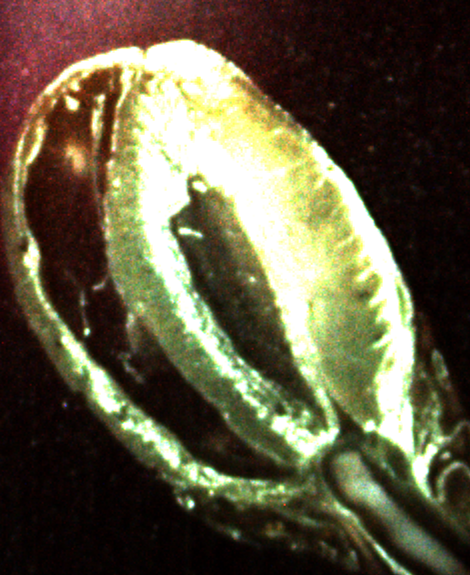
\includegraphics[width=0.4\pagewidth]{Ch6/Figs/pca/LoRes_562}}
            \subfigure[][]{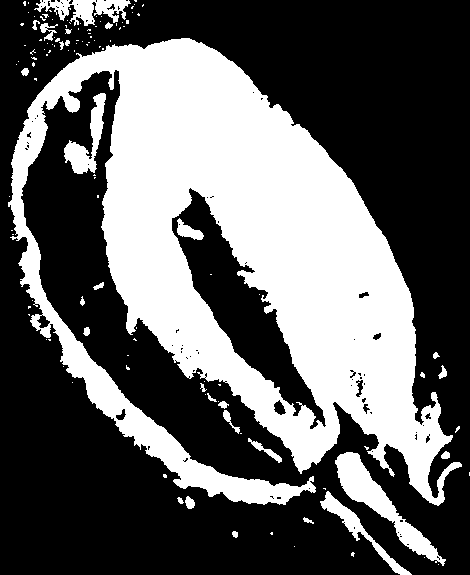
\includegraphics[width=0.4\pagewidth]{Ch6/Figs/pca/LoRes_segmentation_562}}
            \subfigure[][]{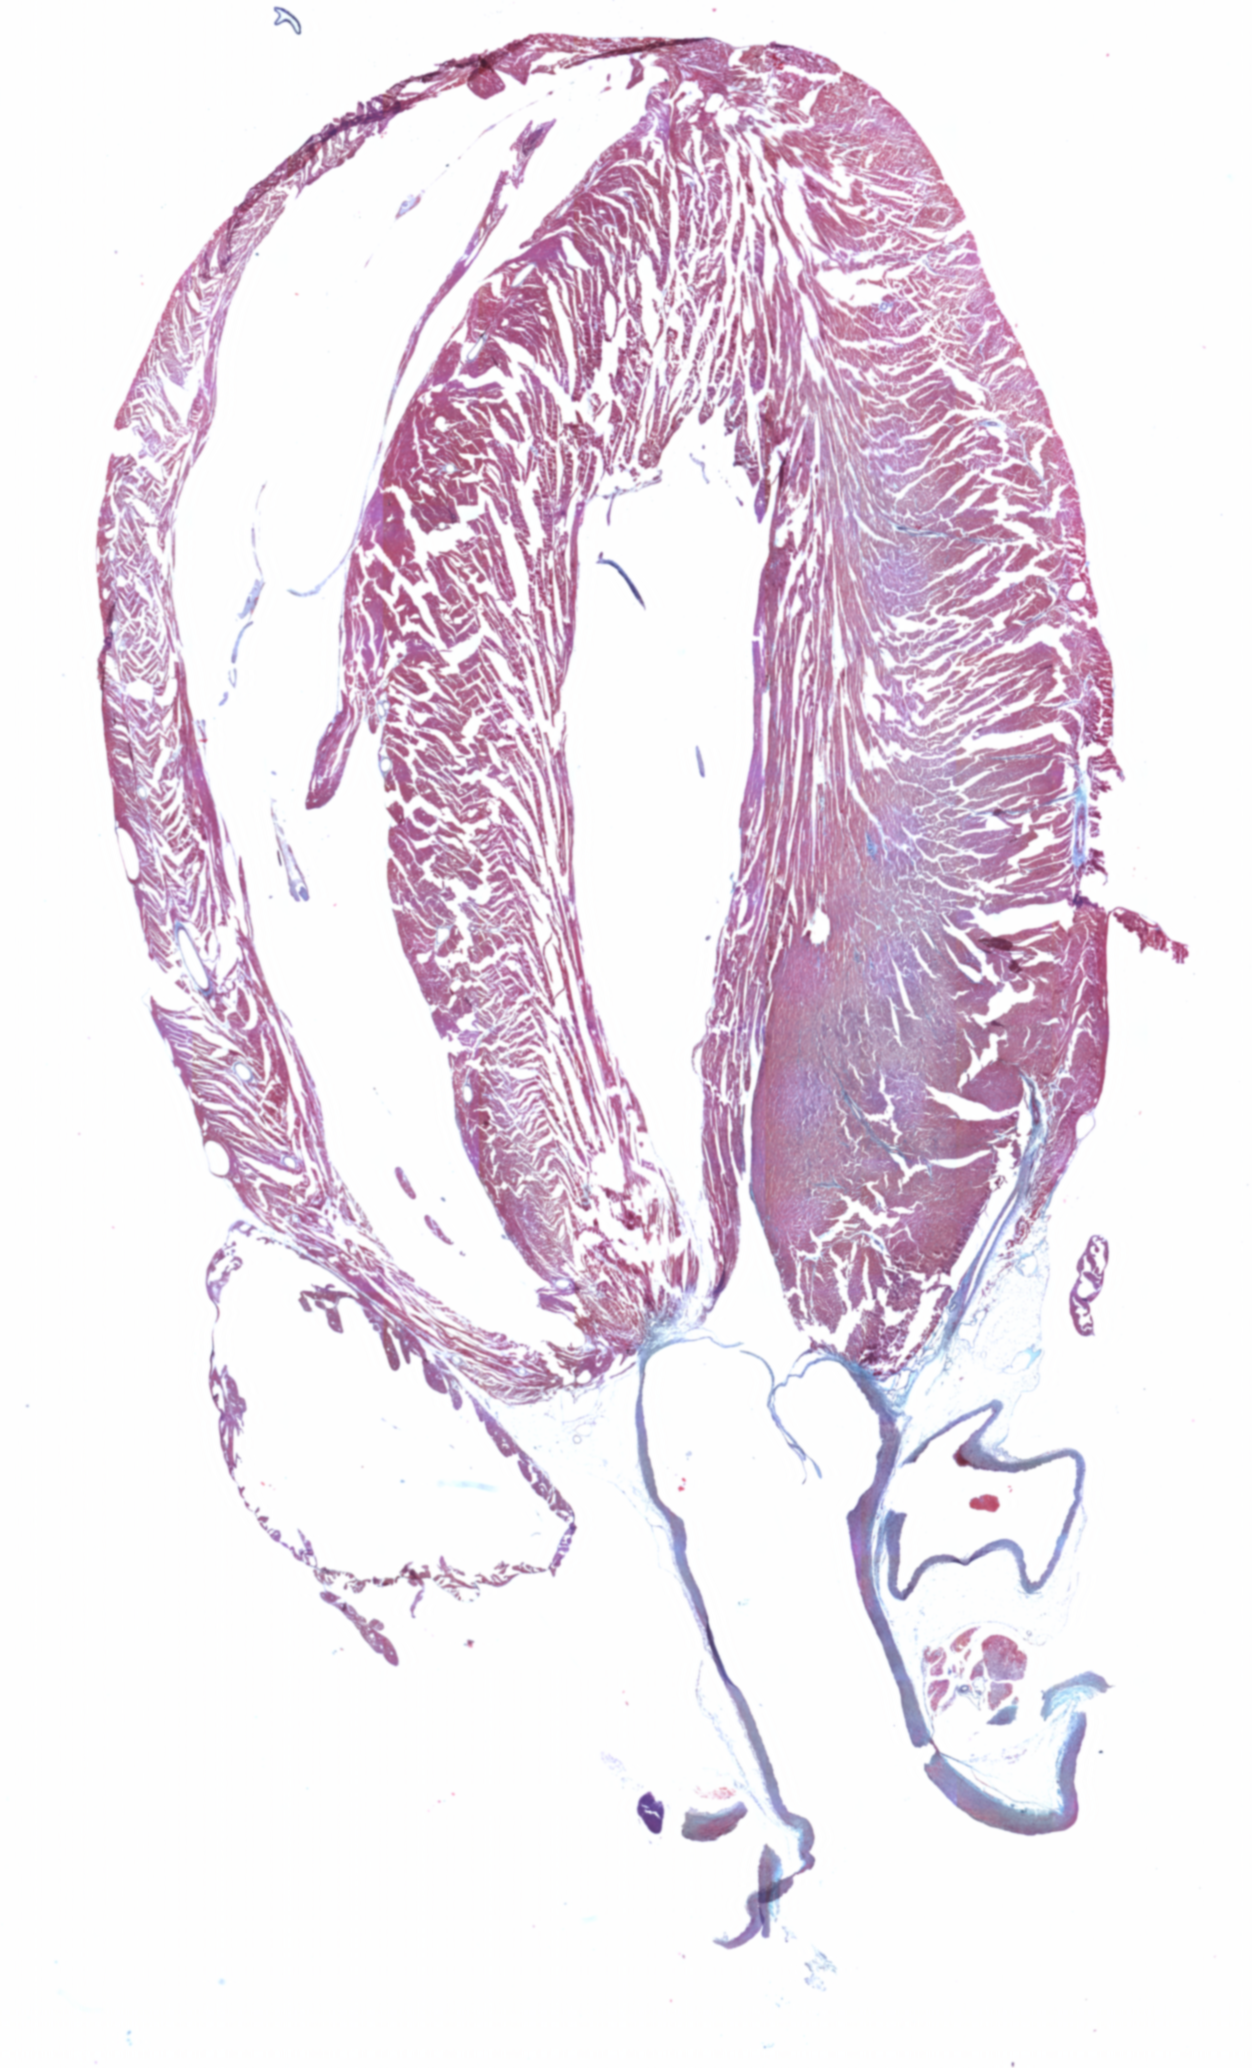
\includegraphics[width=0.4\pagewidth]{Ch6/Figs/pca/HiRes_562}}
            \subfigure[][]{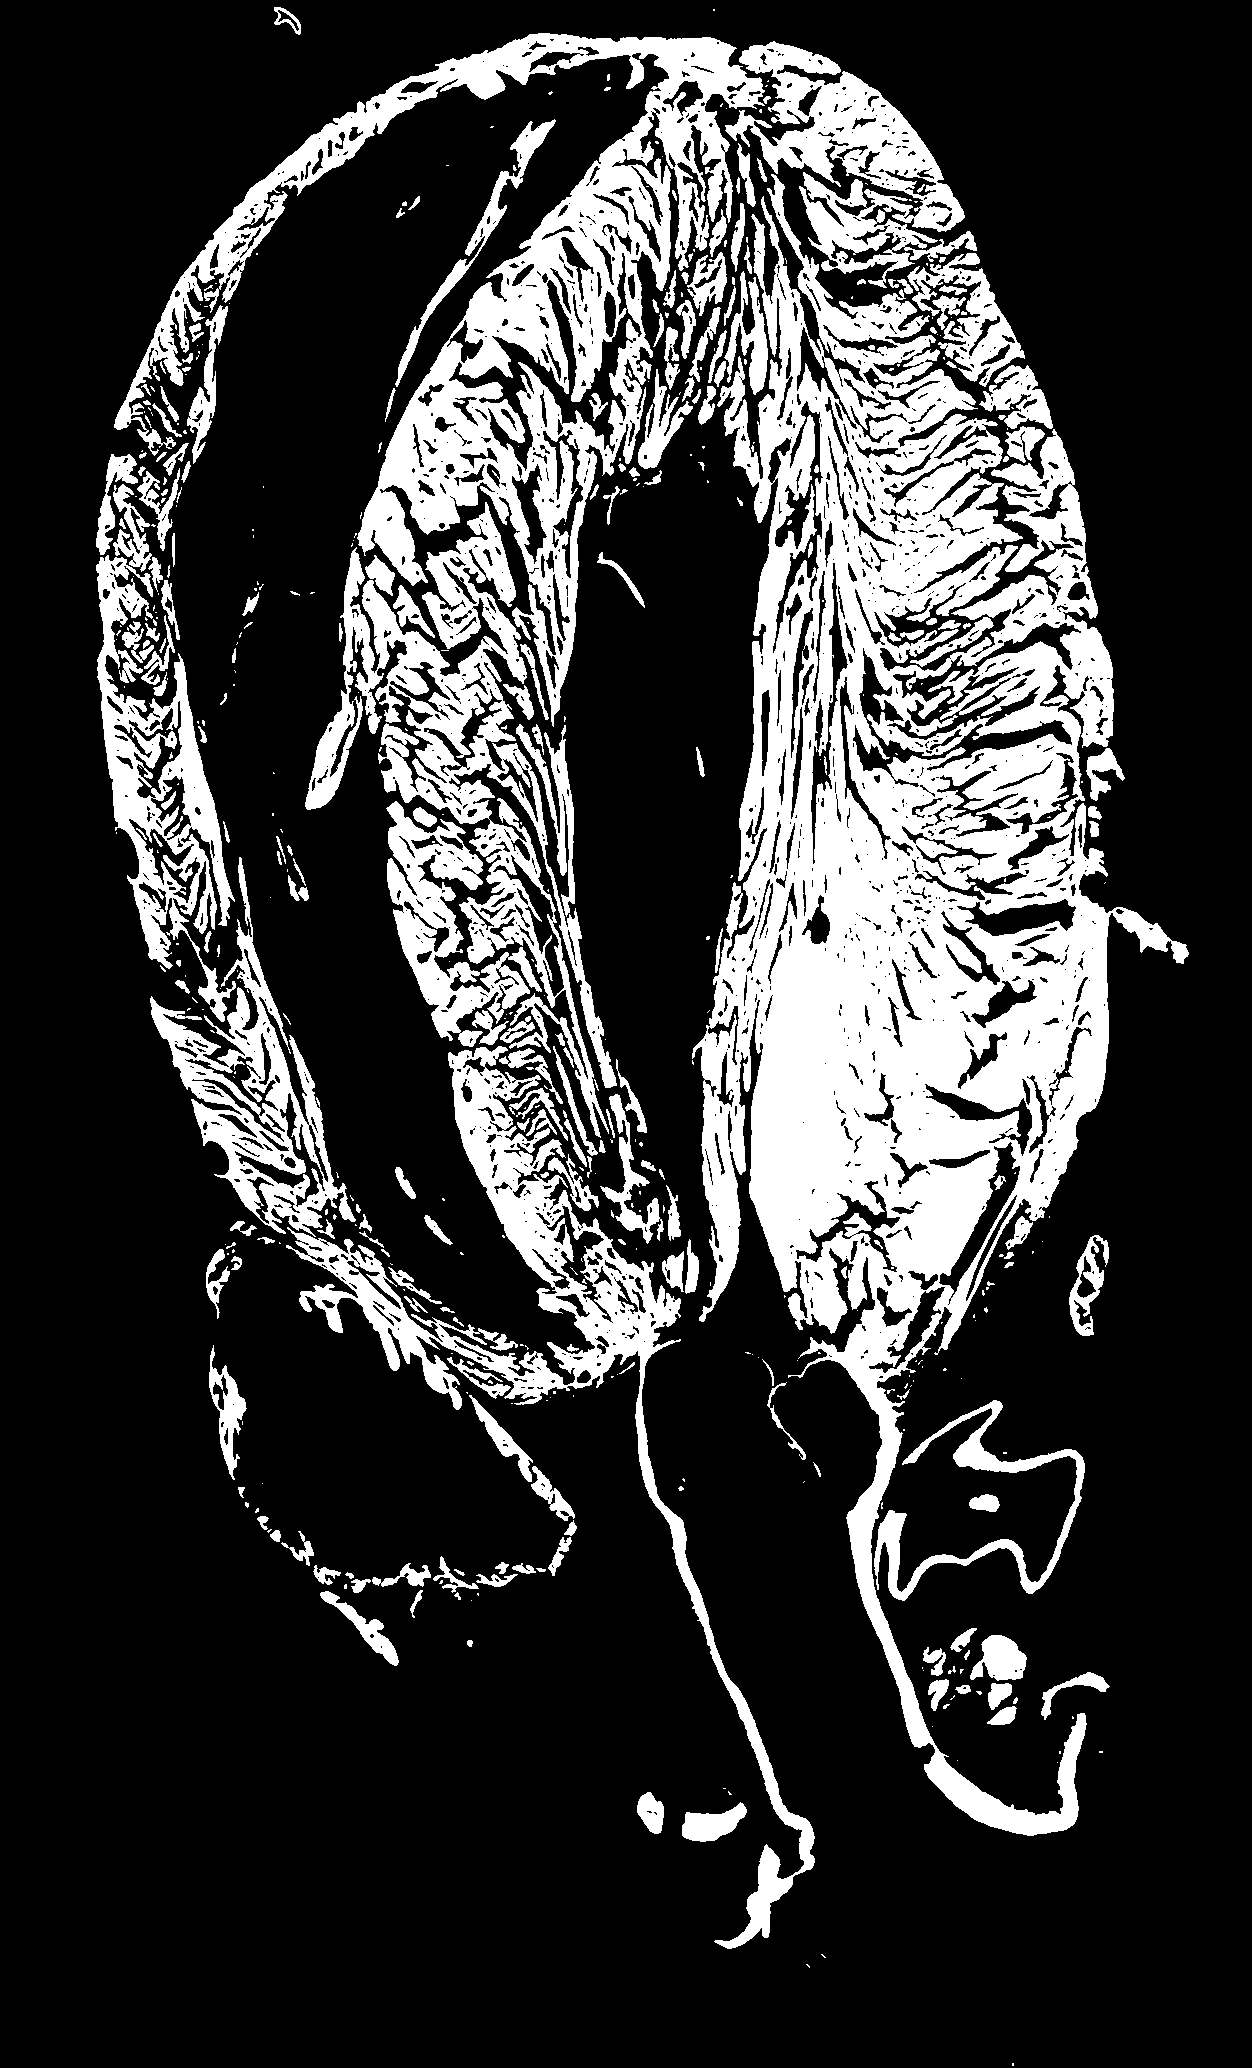
\includegraphics[width=0.4\pagewidth]{Ch6/Figs/pca/HiRes_segmentation_562}}
            \caption{4 figures: LoRes, LoRes segmentation, HiRes, HiRes segmentation}
      \label{fig:segmentation}
    \end{figure}
    
    \begin{figure}[htbp]
      \centering
            \subfigure[][]{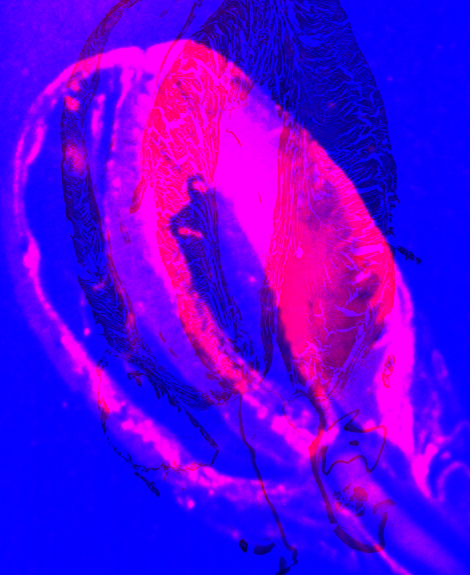
\includegraphics[width=0.4\pagewidth]{Ch6/Figs/pca/geometric_redblue}}
            \subfigure[][]{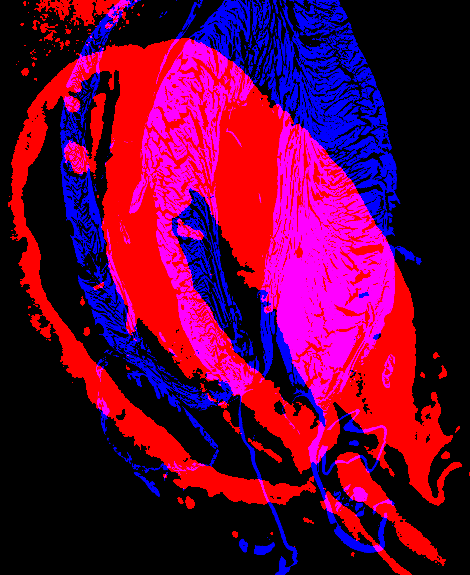
\includegraphics[width=0.4\pagewidth]{Ch6/Figs/pca/geometric_segmentation_redblue}}
            \subfigure[][]{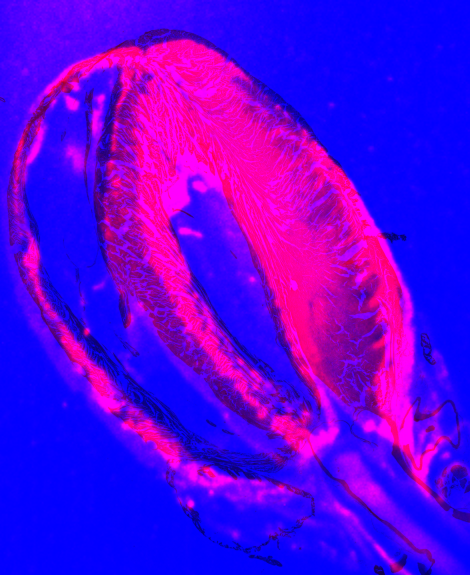
\includegraphics[width=0.4\pagewidth]{Ch6/Figs/pca/pca_redblue}}
            \subfigure[][]{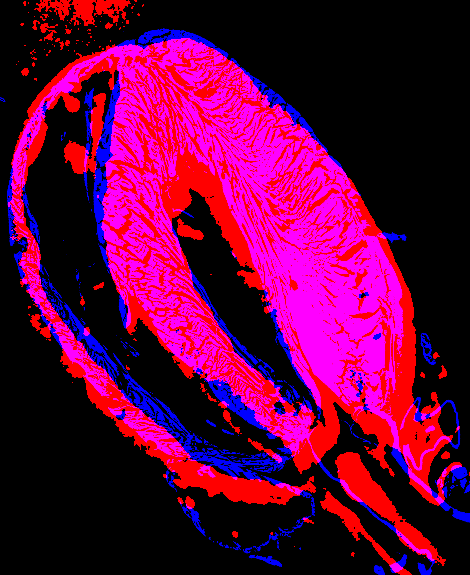
\includegraphics[width=0.4\pagewidth]{Ch6/Figs/pca/pca_segmentation_redblue}}
            \caption{4 figures: RedBlue of Geoms, RedBlue of Geom segmentations, RedBlue of pca, RedBlue of pca segmentations}
      \label{fig:pca}
    \end{figure}
    
    Motivate why the images have to be segmented for pca i.e. empty space shouldn't influence cm, only tissue blah blah.
    
    Write disclaimer somewhere about the unprecedented quality of these images, however unavoidable 
    
    List the issues that plagued both the segmentation and the registration: bubbles, bright blob in top, transmission from layers below, top filamenty bit of heart glowing...
    It is somewhat clear from Figure~\ref{fig:LoRes_cross_sections} that the broad range of tissue colours and intensities in the block face volume overlap significantly with the colours and intensities of non-tissue. In Figures~\labelcref{fig:segmentation,fig:pca}, the threshold segmentation values were optimised for these particular slices as a proof of concept, but this slice was chosen as one of the best examples of the technique. Even if a segmentation method could yield reasonable results for every slice in the dataset, it is impractical to tune parameters manually for each slice, and there would certainly not be a single parameter set suitable for every slice in the volume. For these reasons, the PCA method could not be used to improve robustly upon a simple geometric initialisation of the high-resolution slices seen in Figure~\ref{fig:geometric_initialisation}.
    
    Say that there is no facility to align PCs in ITK, only align centres of mass. Wrote a class to blah blah.
    
    Several methods of segmentation were tried LOOK IN SEGMENTATION PROJECT, INCLUDE DIAGRAM OF LEVEL SETS. It is noted that only the segmentation's moments are of consequence, in particular the centre of mass, and the variance matrix. It is therefore unnecessary for the segmentation to overlap closely with the tissue at a small scale, only that the global distribution of tissue be represented accurately. Go into detail about how the top bit is overrepresented in the LoRes and under in the hires
        
  % subsection initialisation (end)
   
  \subsection{Registration Algorithm} % (fold)
  \label{sub:registration_algorithm}
    A well-founded registration algorithm must embody three traits: numerically, it must reliably converge to the global minimum; computationally, it must be efficient so as to be tractable; and physically, it must correspond to the process that it was designed to correct for. It is within the context of these three benchmarks that we expound the following techniques.
    
    \subsubsection{Transforms} % (fold)
    \label{ssub:transforms}
      Registrations are performed in an iterative fashion, gradually reducing in transformation constraint, starting with a simple rigid transform.
      
SENTENCE ABOUT TRANSFORM COMPLEXITY AND SIZE OF PARAMETER SPACE.  followed by an incrementally increasing transform complexity 

Completing rigid registration before releasing non-rigid degrees of freedom also helps ensure a good starting point in a high-dimensional non-rigid parameter space. 

By far most of the registration is done in the first rigid step. Didn't work for lots of reasons, tried PCA, ITKv3 bug, different metrics, optimisers, normalising images etc. loads of figures.

Show instabilities and scaling factor problems

The sectioning of the slices introduces 2-D, slice-specific deformation and in some cases damage. The subsequent relaxing and rehydration of each slice causes further deformation. Some of this deformation will be of affine form, blah blah

        Transforms were optimised in the following order, the final result of each initialising its successor: a centred rigid 2D transform - a rotation about an arbitrary centre followed by a translation; a centred similarity transform - as before but with a scaling factor; a centred affine transform - an affine transformation around an arbitrary centre followed by a translation; a coarse grid bspline deformable transform; and a fine grid bspline deformable transform. For all centred transforms, the centre of rotation was exposed for optimisation as metric parameters.
    % subsubsection transforms (end)
    
    \subsubsection{Optimisation} % (fold)
    \label{ssub:optimisation}
      Gradient Descent (GD) and Regular Step Gradient Descent (RSGD) optimisers have been applied. RSGD terminates before the maximum number of iterations has passed, and so in simple cases it is computationally more efficient. In most scenarios, however, the GD optimiser often proves more robust. In both cases, a choice to maximise or minimise the cost function must be chosen, the latter being dependent on both the choice of metric and the preconditioning of the image intensity ranges.

      The optimisation space, as dictated by the transform, must be scaled along each dimension to correct for discrepant effects per unit change of each parameter. For example, a translation of one micron at the epicardium might result from a rotation of just $10^{-5}$ radians about the centre of the slice. This makes the metric space more isotropic and reduces the eccentricity of cost function basins, allowing the optimisation algorithm to fall more directly towards minima.
    % subsubsection optimisation (end)
    
    \subsubsection{Metrics} % (fold)
    \label{ssub:metrics}
      Mutual Information (MI) is usually considered to be most effective when registering images from different modalities. However, after a plethora of parameterisations and configurations was explored based on this metric, incrementally simpler and simpler metrics were tested. Each demanded more image preconditioning and tuning, but yielded monotonically closer and more consistent registrations, with a larger capture range, and required fewer iterations to converge. First, a normalised correlation was employed, with the simplest mean squares difference algorithm proving most suitable. It would appear that the simpler the intensity relationship, the smoother the cost landscape, with fewer local minima.
      
      The mutual information metric is highly suitable for matching different modalities, the downsampling of the images acts to smooth out the optimised function and prevent trapping in local minima, and the optimisation algorithm is a good choice for an unknown topology. 
      
      
      Typically, large capture regions are associated with low precision for the maximum, so it may prove beneficial to revert to MI for the final bspline registration.
    % subsubsection metrics (end)
    
    \subsubsection{Intensity Scaling} % (fold)
    \label{ssub:intensity_scaling}
      In order for the mean squares image metric to perform, the intensities of one of the image sets needed to be remapped beforehand such that there was a positive linear intensity correlation between equivalent points in the tissue. To this end, a histogram matching algorithm was applied to the slice volume based on the intensities from the block face volume. DISCUSS CONSTRAINTS OF DIFFERENT METRICS
    % subsubsection intensity_scaling (end)
    
    \subsubsection{Interpolation} % (fold)
    \label{ssub:interpolation}
      ITK provides four methods of interpolation: nearest neighbour, linear, B-spline and windowed sinc. Nearest neighbour interpolation simply returns the value of the closest pixel in the image being sampled. This requires the least amount of computation of the four methods, but results in a more jagged optimisation function, which could increase the time to convergence, the exact value converged upon, or in rare cases could prevent convergence to the global minimum. More accurately, but slightly more expensively, the value can be linearly interpolated from the four corners of the containing square or eight of the containing cube. Even more accurately, the image intensity can be calculated using B-spline basis functions. However, values may lie outside the range of input image intensities, causing saturation. Finally, the most accurate is the windowed sinc interpolator. Interpolation is based on the Fourier analysis of a sampled smooth spatial function. The pixel intensity is the result of a convolution of the sinc function with a window of neighbouring pixels. This requires by a stretch the most computation. For our purposes, linear interpolation provided the best compromise between efficiency and accuracy.
    % subsubsection interpolation (end)
    
    \subsubsection{Metric} % (fold)
    \label{ssub:metric}
      The metrics available in ITK compare the gray-scale intensity of two images to measure how well they are aligned. Masks can be set for both the fixed and moving images to restrict evaluation of the metric within a specified region. The choice of metric critically affects the shape of the optimisation function in the parameter space, and some are only suitable to compare images of the same modality. A mean squares metric requires that equivalent points in the two images are at the same intensity in order to function well. A normalised correlation metric is slightly more flexible in its range of application, but still assumes a linear relationship between equivalent intensities in the two images. A mutual information metric assumes no such relationship. The mutual information between two images is a measure of how much information a random intensity from one image confers about the intensity at the equivalent point in the other image. For example, a region could be uniquely dark grey in one image, but uniquely red in the other. Regardless of the colour or intensity, if a randomly selected pixel turns out to be that exact dark grey in the first image, one can be sure that the same point in the second image is red, and vice versa; mutual information is maximised. If for some reason, these regions were misaligned, that certainty is compromised, and the contribution to the mutual information coefficient from that region is reduced. The mutual information approach is ideally suited to the registration of MRI to histology, where the relationship between intensities is highly complex.
    % subsubsection metric (end)
    
    \subsubsection{Optimisation} % (fold)
    \label{ssub:optimisation}
      The optimiser iteratively moves through the space defined by the transform parameters from a set of initial coordinates, in an attempt to minimise the cost function evaluated by the metric. ITK provides a range of algorithms to achieve this task in the most efficient and reliable way possible. Throughout the registration process, a gradient descent optimiser was employed. This optimiser is a robust, general purpose algorithm that requires little configuration.
    % subsubsection optimisation (end)
  % subsection registration_algorithm (end)
  
  \subsection{Software Architecture} % (fold)
  \label{sub:software_architecture}
    MOTIVATE SOFTWARE QUALITY SECTION, SAY PROBLEMS I HAD, Discuss why, because the final result is unknown, any bugs or errors in calculation are often not apparent, and very difficult to find. Maybe anecdote about a slight error in calculating the initial centre of rotation for transforms went 9 months unnoticed. QUOTE VARIOUS SOFTWARE PRINCIPLES E.G. DRY, SINGLE POINT OF TRUTH,

    All file handling and networking algorithms were written in Ruby, a powerful, object-oriented, all-purpose, cross-platform scripting language. YAML (YAML Ain't a Markup Language) was used as a declarative language for configuration files, providing a syntax that is easily human readable and curatable, yet machine parsable. The main use of YAML was to store metadata for each histological slice, such as whether the image was flipped, whether it was trichrome stained, and the nature and extent of any damage or abberation. Source code management and code deployment was implemented in Git. All imaging algorithms were written in C++, using the venerable ITK library. C++ executables were compiled using the cross-platform build system CMake, an open source program and project founded by the same organisation that started ITK.
    
    An outline of the main problems encountered during the development process will be exhibited, along with the solutions crafted to overcome them.
    
    \subsubsection{Multiresolution Registration} % (fold)
    \label{ssub:multiresolution_registration}
      SECTION ON MULTIRESOLUTION, BOTH IN PLANE AND WITH IMAGE LISTS. TALK ABOUT REPRESENTATIVE SETS OF SLICES 100-110 + 200-210 + 300-310 ETC. TALK ABOUT TRACTABILITY WITH IMAGE SIZE AND TIME FOR REGISTRATION, AND HOW EACH ALGORITHM WAS SPLIT UP INTO INDIVIDUAL SLICES
      
	  The full-resolution histology dataset can measure 2TB
	  
      Motivate multires: state figures on total size of dataset, and on total times and memory to run 1 registration on a laptop and on a supercomputer. Talk about high dimensionality of parameter space, and the need for rapid feedback if the right parameters are to be found in any reasonable time.
    
      There are 2 ways to achieve this: in-plane downsampling and out-of-plane slice selection. Downsampling and Gaussian smoothing not only reduces time, but smooths the cost function and can lead to more robust registration results. In multiresolution registration, the resulting transforms can then be used to initialise a more accurate but more fragile registration at a higher resolution.
    
    % subsubsection multiresolution_registration (end)
    
    \subsubsection{Stacks} % (fold)
    \label{ssub:stacks}
            Histology data are provided in series of 2D png images. Images within a set can each be of unique size, and slices which were damaged or which have not been imaged yet are missing. Each block image must be paired with its equivalent slice image, and blank images must be interpolated where images are missing. Slices must be transformed independently and by a range of transforms. Binary masks must be generated for each image, so that metrics will only take pixel intensities into account from inside the boundaries of the original untransformed images. A minimum percentage overlap is required for many metrics to function, and for small slice images close to the apex of the heart, block mask areas must be cropped until this constraint is satisfied.

            The Stack has been developed to encapsulate the solutions to all of these problems. A Stack represents the 3D composition of a set of 2D slices. It handles ROI selection, generic transform storage, image and mask resampling and generation (both for 2D slices and for the 3D volume) and various error handling strategies. An MRI class is also available to solve the complementary problem of extracting arbitrarily oriented slices from a 3D image. However, for these specific datasets the block face images are intrinsically registered to the histological samples.
    
      A `mask' is also generated, a binary image of the same dimensions as the volume stack, with value 1 within a histological slice, and zero otherwise. The mask is used by the metric to specify which pixels will be taken into consideration.
    % subsubsection stacks (end)
    
    \subsubsection{Pipeline Builders} % (fold)
    \label{ssub:pipeline_builders}
      MAYBE RENAME SUBSUBSECTION TO MORE GENERIC `BUILDERS'...SEARCH THROUGH SOURCE CODE FOR OTHER TYPES OF BUILDERS
          A minimal registration pipeline is composed of several generic actors, including a metric, an optimiser, a transform, and an interpolator. The details of which types of actors are optimal and how they should interact are peculiar to the registration problem at hand. Furthermore, the specific type of each component often requires unique configuration beyond the generic interface of its family. Once several types must be chosen from and configured, even for just one component, an ad hoc procedural approach quickly became unwieldy, but these two requirements colluded combinatorially to demand a great deal of testing, tailoring and configuration in order to achieve registrations of high quality. More often than not, modifications would degrade the registration, and reversing parts of them proved non-trivial.

          At the pipeline level, we developed a heirarchy of `frameworks' employing the Builder pattern, which abstracts away the heavy lifting of wiring up the various components together.  At the component level, a conflation of the Abstract Factory and the Strategy patterns, together with a configuration system using the human-friendly YAML markup language, serves not only to decouple the actors' representations from the minutiae of their construction, but to move these volatile decisions from compile-time to runtime. These tools vastly reduce the cost of experimentation and testing. With all the variables clearly grouped together, with no need to recompile the toolchain or pore through source code to find if and where one can make a change, the feedback from results is faster and less error prone.

      
    % subsubsection pipeline_builders (end)
        \paragraph{Component Builders}
        Should this go in here? or in the paper?

        \paragraph{Checkpointing and Transform IO}
          At any stage during the registration process, the vector of transforms held by a given Stack can be persisted to a file or a series of files with a single function call. Just as easily, a new Stack can be initialised with a set of transforms on storage. This machinery facilitates greater process granularity in three dimensions: in the sequence of transforms to be optimised, in the increasing image resolutions to be registered, and spatially in the pairs of slices within the Stack. In the first case, a user can tune one registration stage until they are happy that it is optimal, and then use the results as a starting point for all subsequent runs of the next stage. Moreover, the division of workload and memory is of particular importance when organising jobs on clusters and shared memory machines. ALSO TALK ABOUT COMPOSING TRANSFORMS RATHER THAN REPEATED RESAMPLING PREVENTS A LOSS OF IMAGE QUALITY DUE TO REPEATED RASTERISATION IN DIFFERING COORDINATE SYSTEMS. TALK ABOUT DIFFERENT PIXEL TYPES: FLOAT/DOUBLE PIXEL TYPES CAN BE USED FOR ACCURATE INTERPOLATION OF INTENSITIES DURING REGISTRATION, THEN THE TRANSFORMS CAN BE USED TO RECONSTRUCT A COLOUR VOLUME OR A SEGMENTATION AFTERWARDS.
          
          \vspace{3 mm}

          Several other aspects of the architecture are not discussed here, including Configuration, File Management, Logging Output, Testing, as well as the opportunities and challenges posed by high performance computing.
    
  % subsection software_architecture (end)
  
    \subsection{Diagnostics} % (fold)
    \label{sub:diagnostics}
      
      MOTIVATION: For a year and a half, very difficult to see why registration was failing. Output of raw parameters got us somewhere, but only for obvious issues e.g. parameter scaling, step length. Huge parameter space. Sports game analogy about result, but no play-by-play. BuildProgressVolumes
      
      IN ORDER TO OUTPUT INTERMEDIATE TRANSFORMS AND METRIC VALUES AT EACH ITERATION, WAS NECESSARY TO HOOK INTO ITK'S EVENT-DRIVEN API, USING THE COMMAND-OBSERVER PATTERN (CITE GANG OF 4). PERHAPS QUICK OMNIGRAFFLE FIGURE OF OBSERVER HEIRARCHY?
      
      Parameter tuning:
      
      Figures of bad params, symptoms and results. e.g. zigzags, overshoot and gradual worsening. Unclear how the gradual worsening happens; could be an oddly shaped v-shaped cost basin, deepening steeply along one dimension and 
      
      Before upgrade to ITKv4, registration algorithm would often not optimise i.e. results were much worse. Even though the upgrade shouldn't have affected the results, just the speed of the code, results were much much better.
      
      Parameter tuning:
      Initial discussion of 4 parameters in RSGD: 2 behavioural (max step and relaxation factor), and 2 cutoff(min step and gradient magnitude tolerance).
      Figures need to compare:
        increase/decrease in behavioural (zigzag if too high because of overshoot)
      increase/decrease in cutoff (takes too long if low, see tails in plot metric values and differences, doesn't finish if too high, use compare final metric values.py)

      Increase max step for HiRes pairs registration to 60, and show characteristic zigzagging and jumping out of potential well
      
      \begin{sidewaysfigure}[htbp]
        \centering
        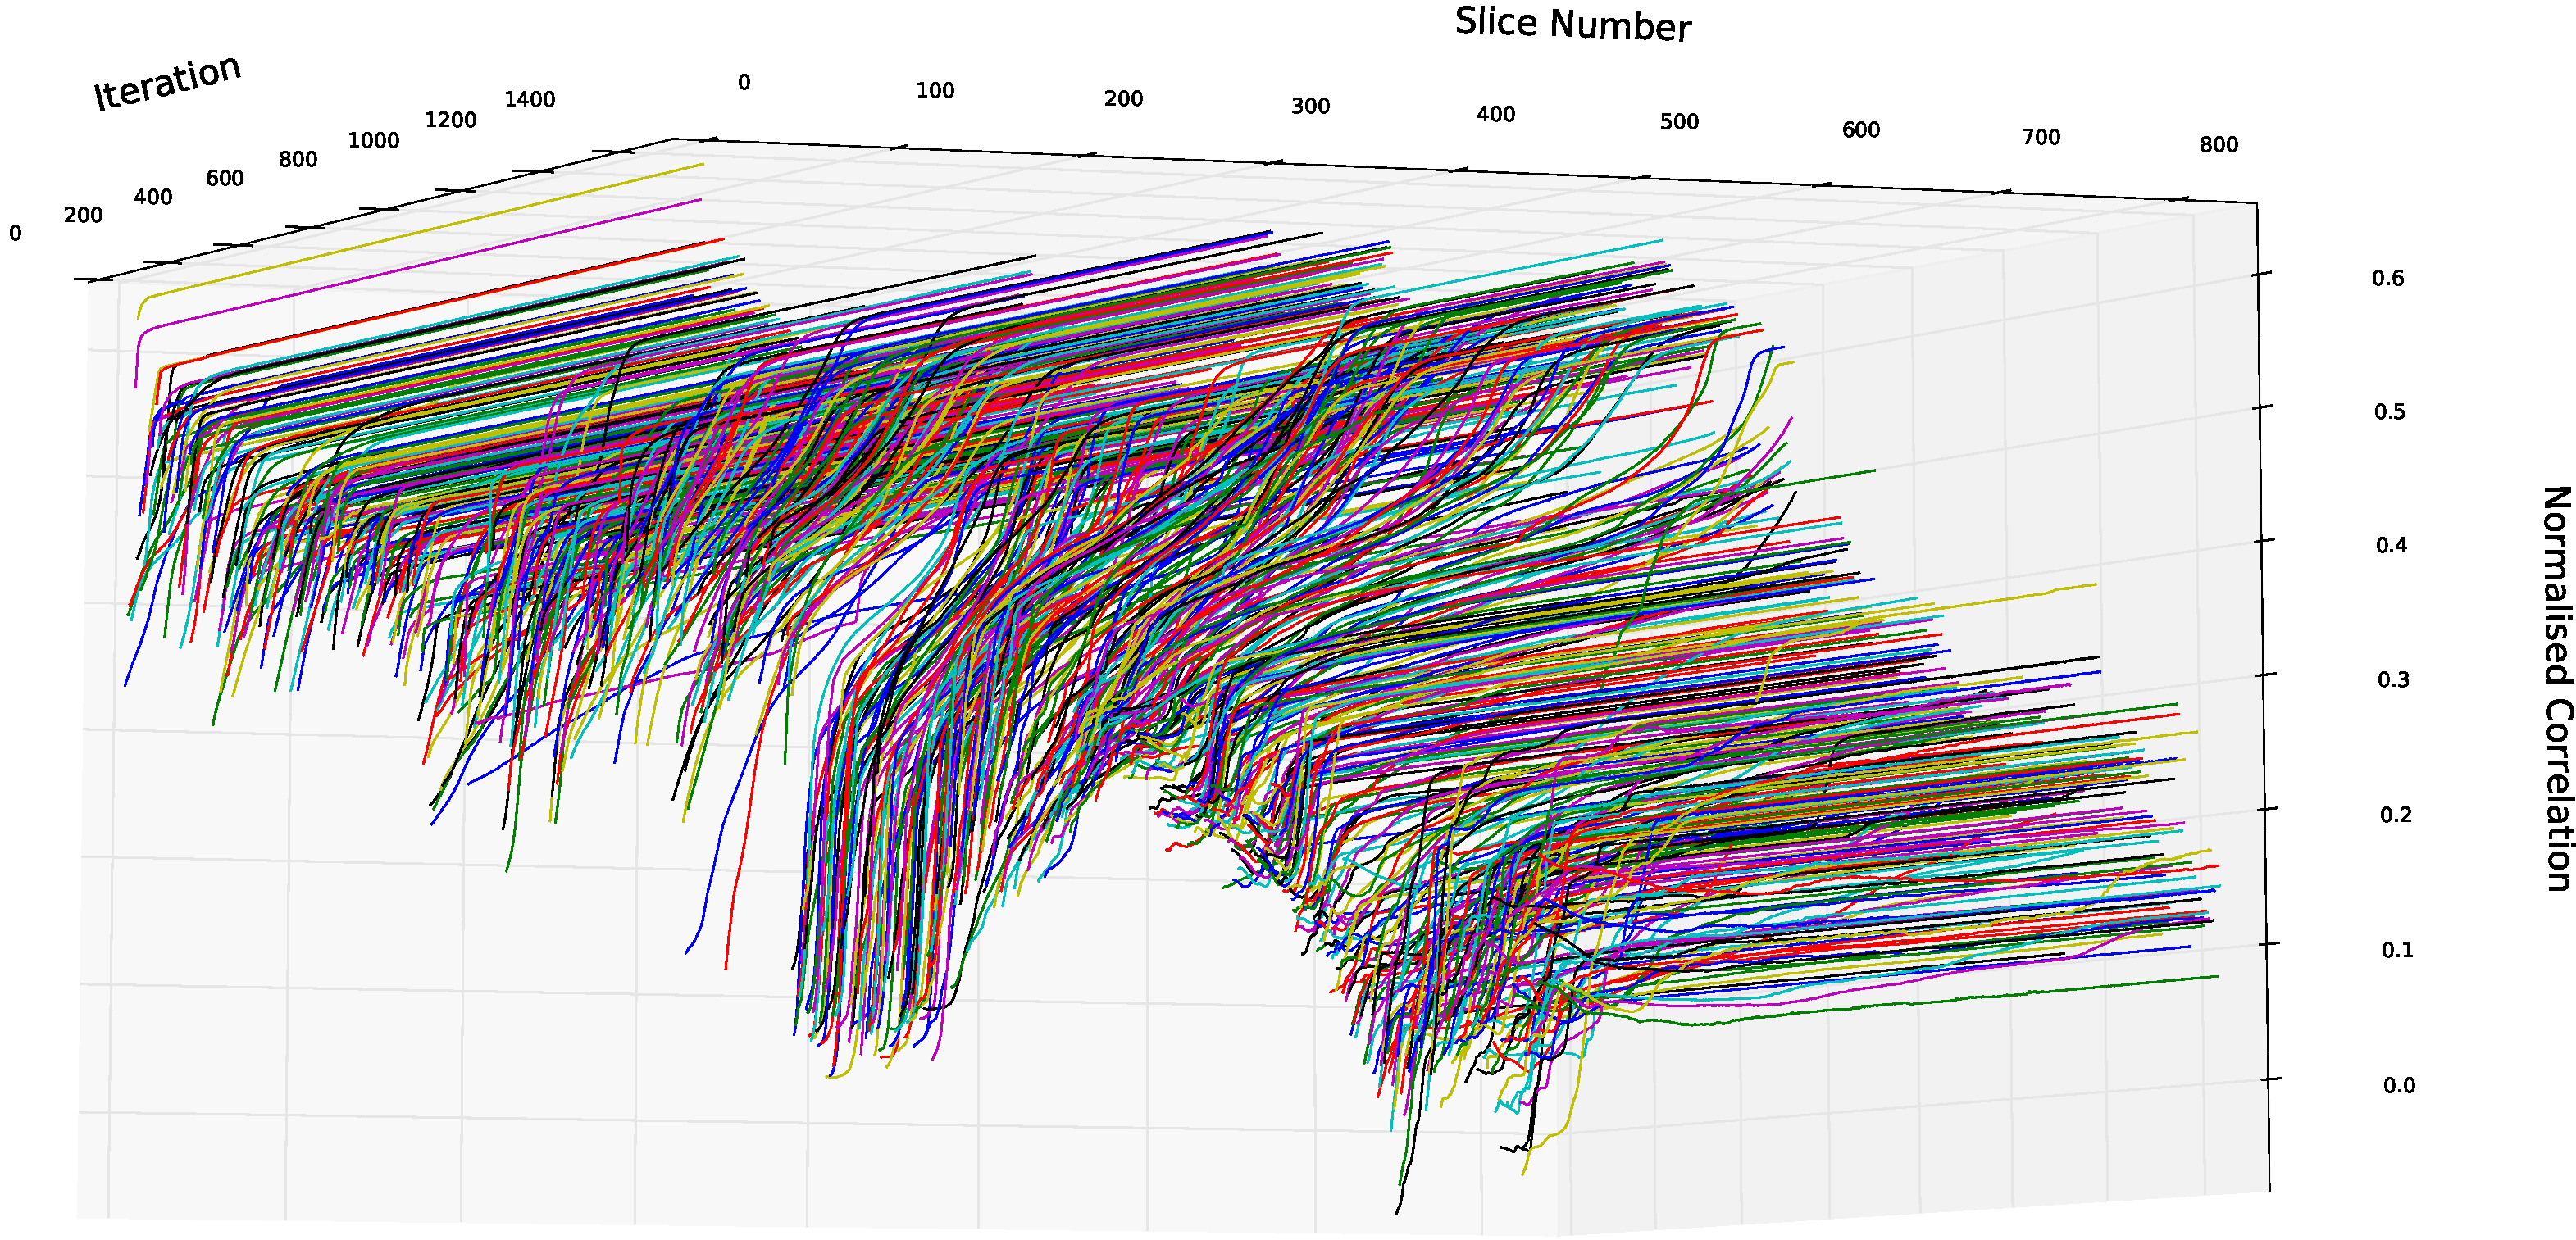
\includegraphics[width=\textheight]{Ch6/Figs/diagnostics/rigid_metric_values}
        \caption{Viewed from below to see clearly all the values. Nearly all curves smoothly and monotonically increase, before reaching a distinct flat maximum. After around slice 600, where blob appears, final metric values decrease almost linearly as the intensity of the blob increases. Slices in the region of 400-600 start from a much lower metric value, and take up to 1500 iterations to maximise. Diagnostics were important here, to see whether all slices had reached maximum. Give times to run 1500 iterations on supercomputer.}
        \label{fig:rigid_metric_values}
      \end{sidewaysfigure}
      
      \begin{sidewaysfigure}[htbp]
        \centering
        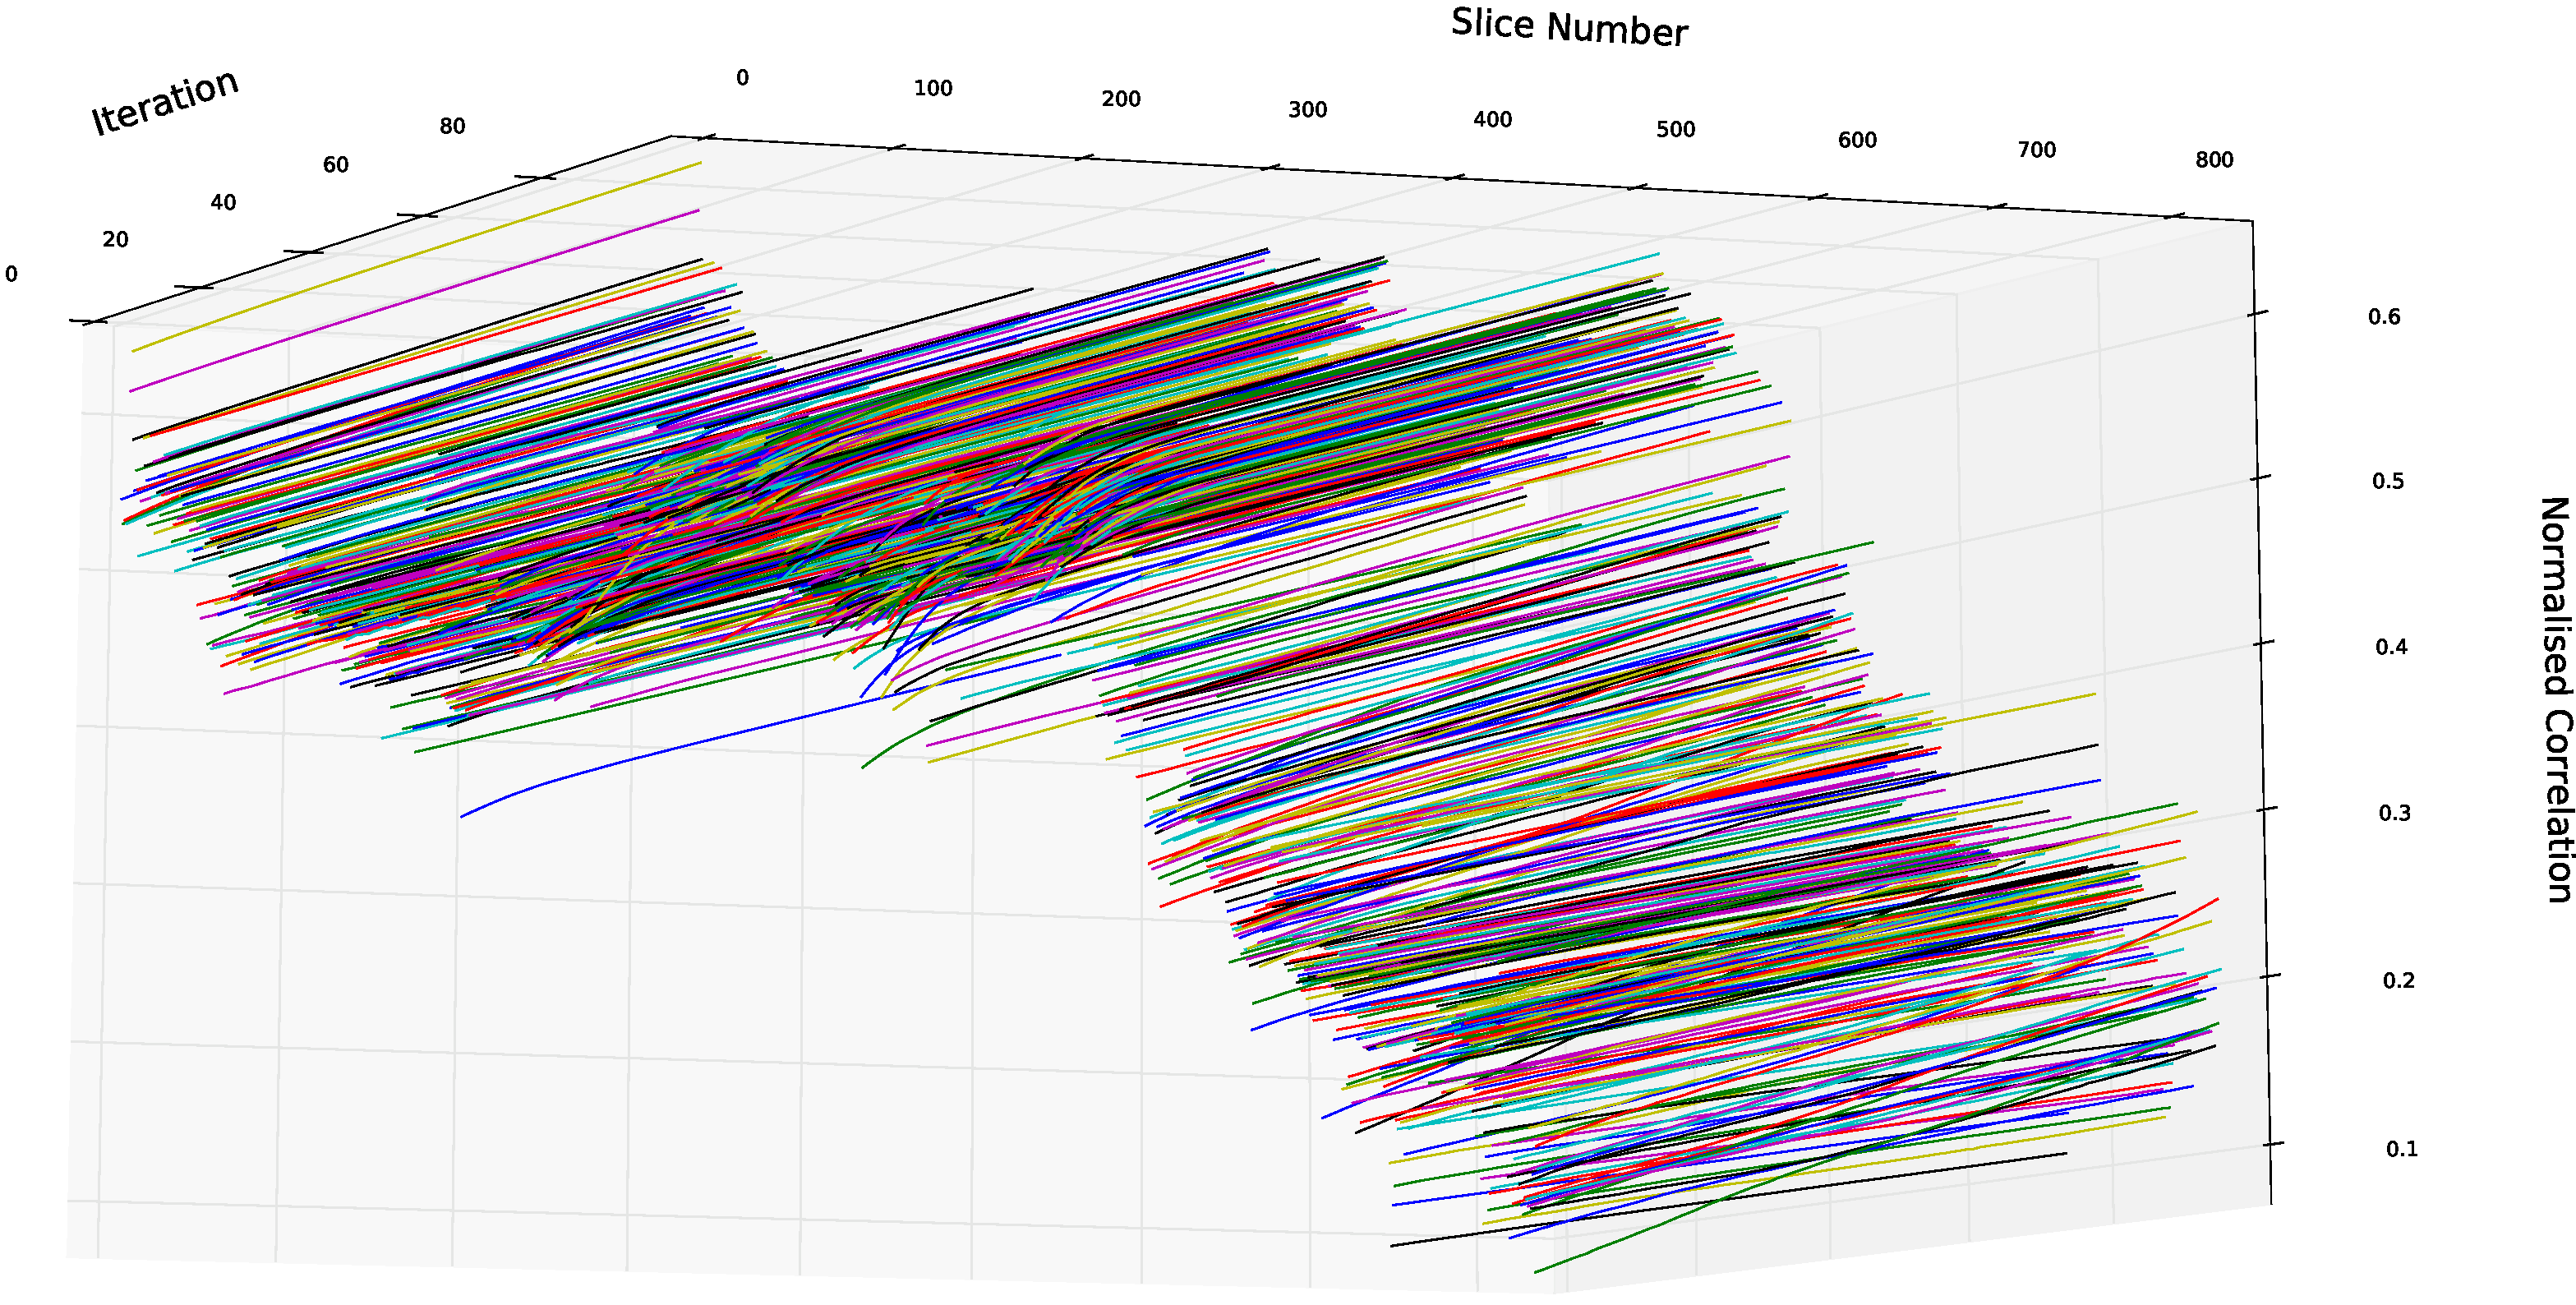
\includegraphics[width=\textheight]{Ch6/Figs/diagnostics/similarity_metric_values}
        \caption{}
        \label{fig:similarity_metric_values}
      \end{sidewaysfigure}
      
      \begin{sidewaysfigure}[htbp]
        \centering
        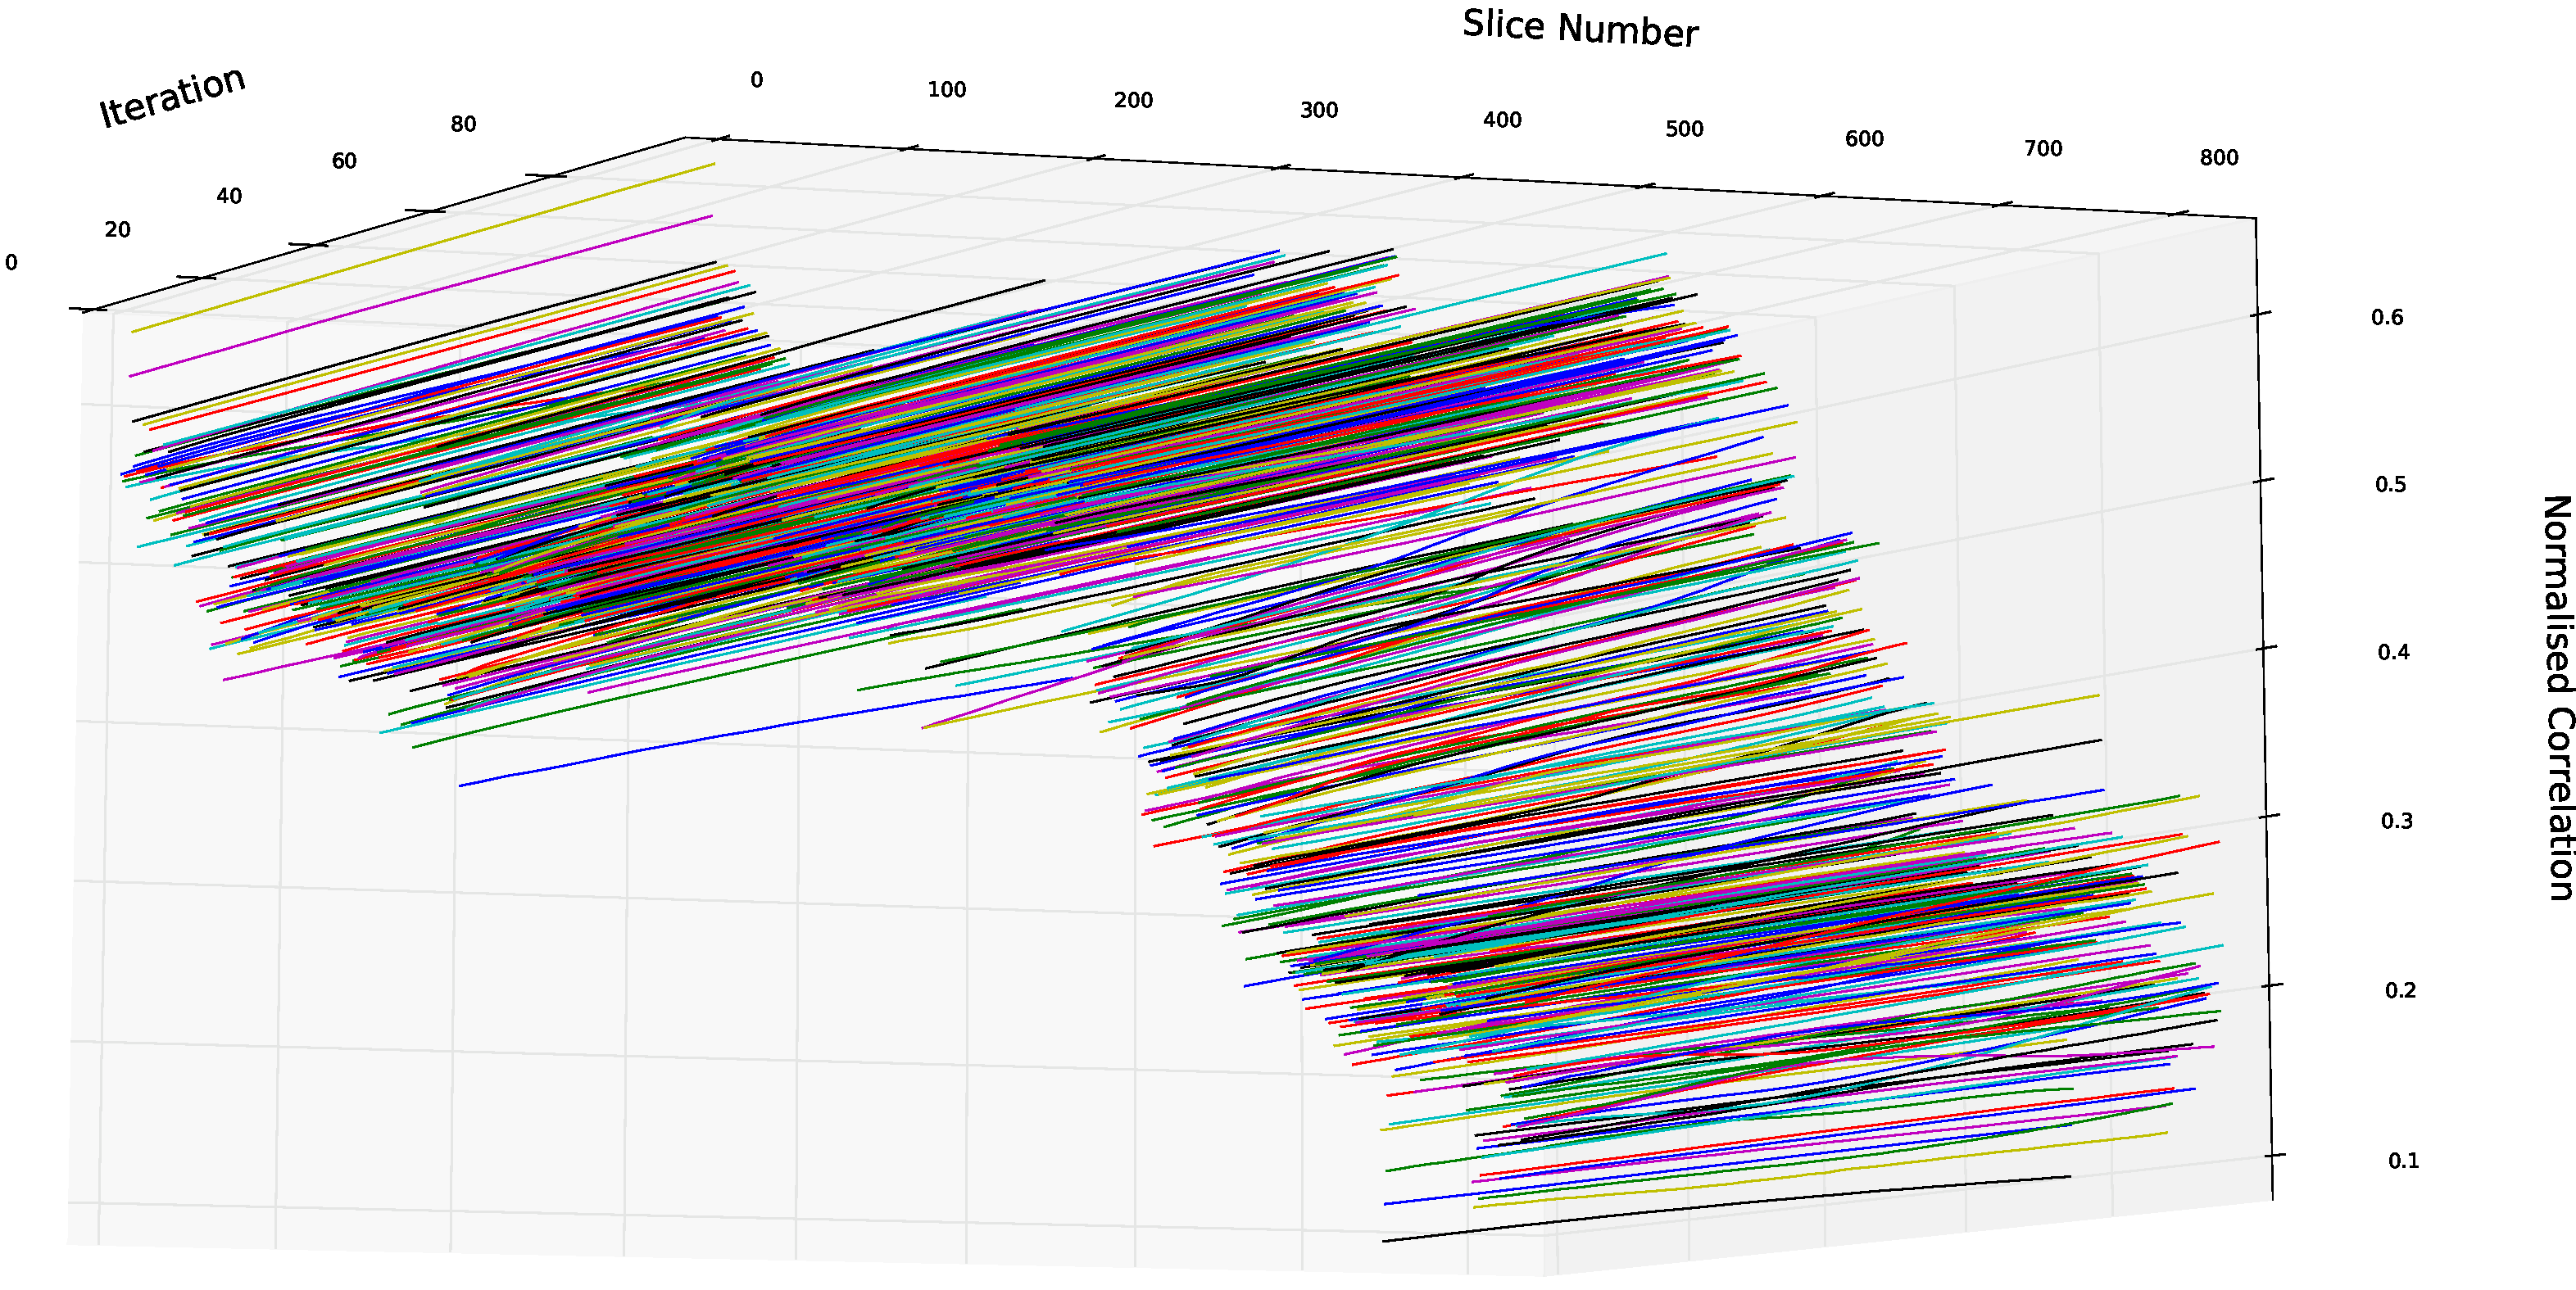
\includegraphics[width=\textheight]{Ch6/Figs/diagnostics/affine_metric_values}
        \caption{}
        \label{fig:affine_metric_values}
      \end{sidewaysfigure}
      
      \begin{sidewaysfigure}[htbp]
        \centering
        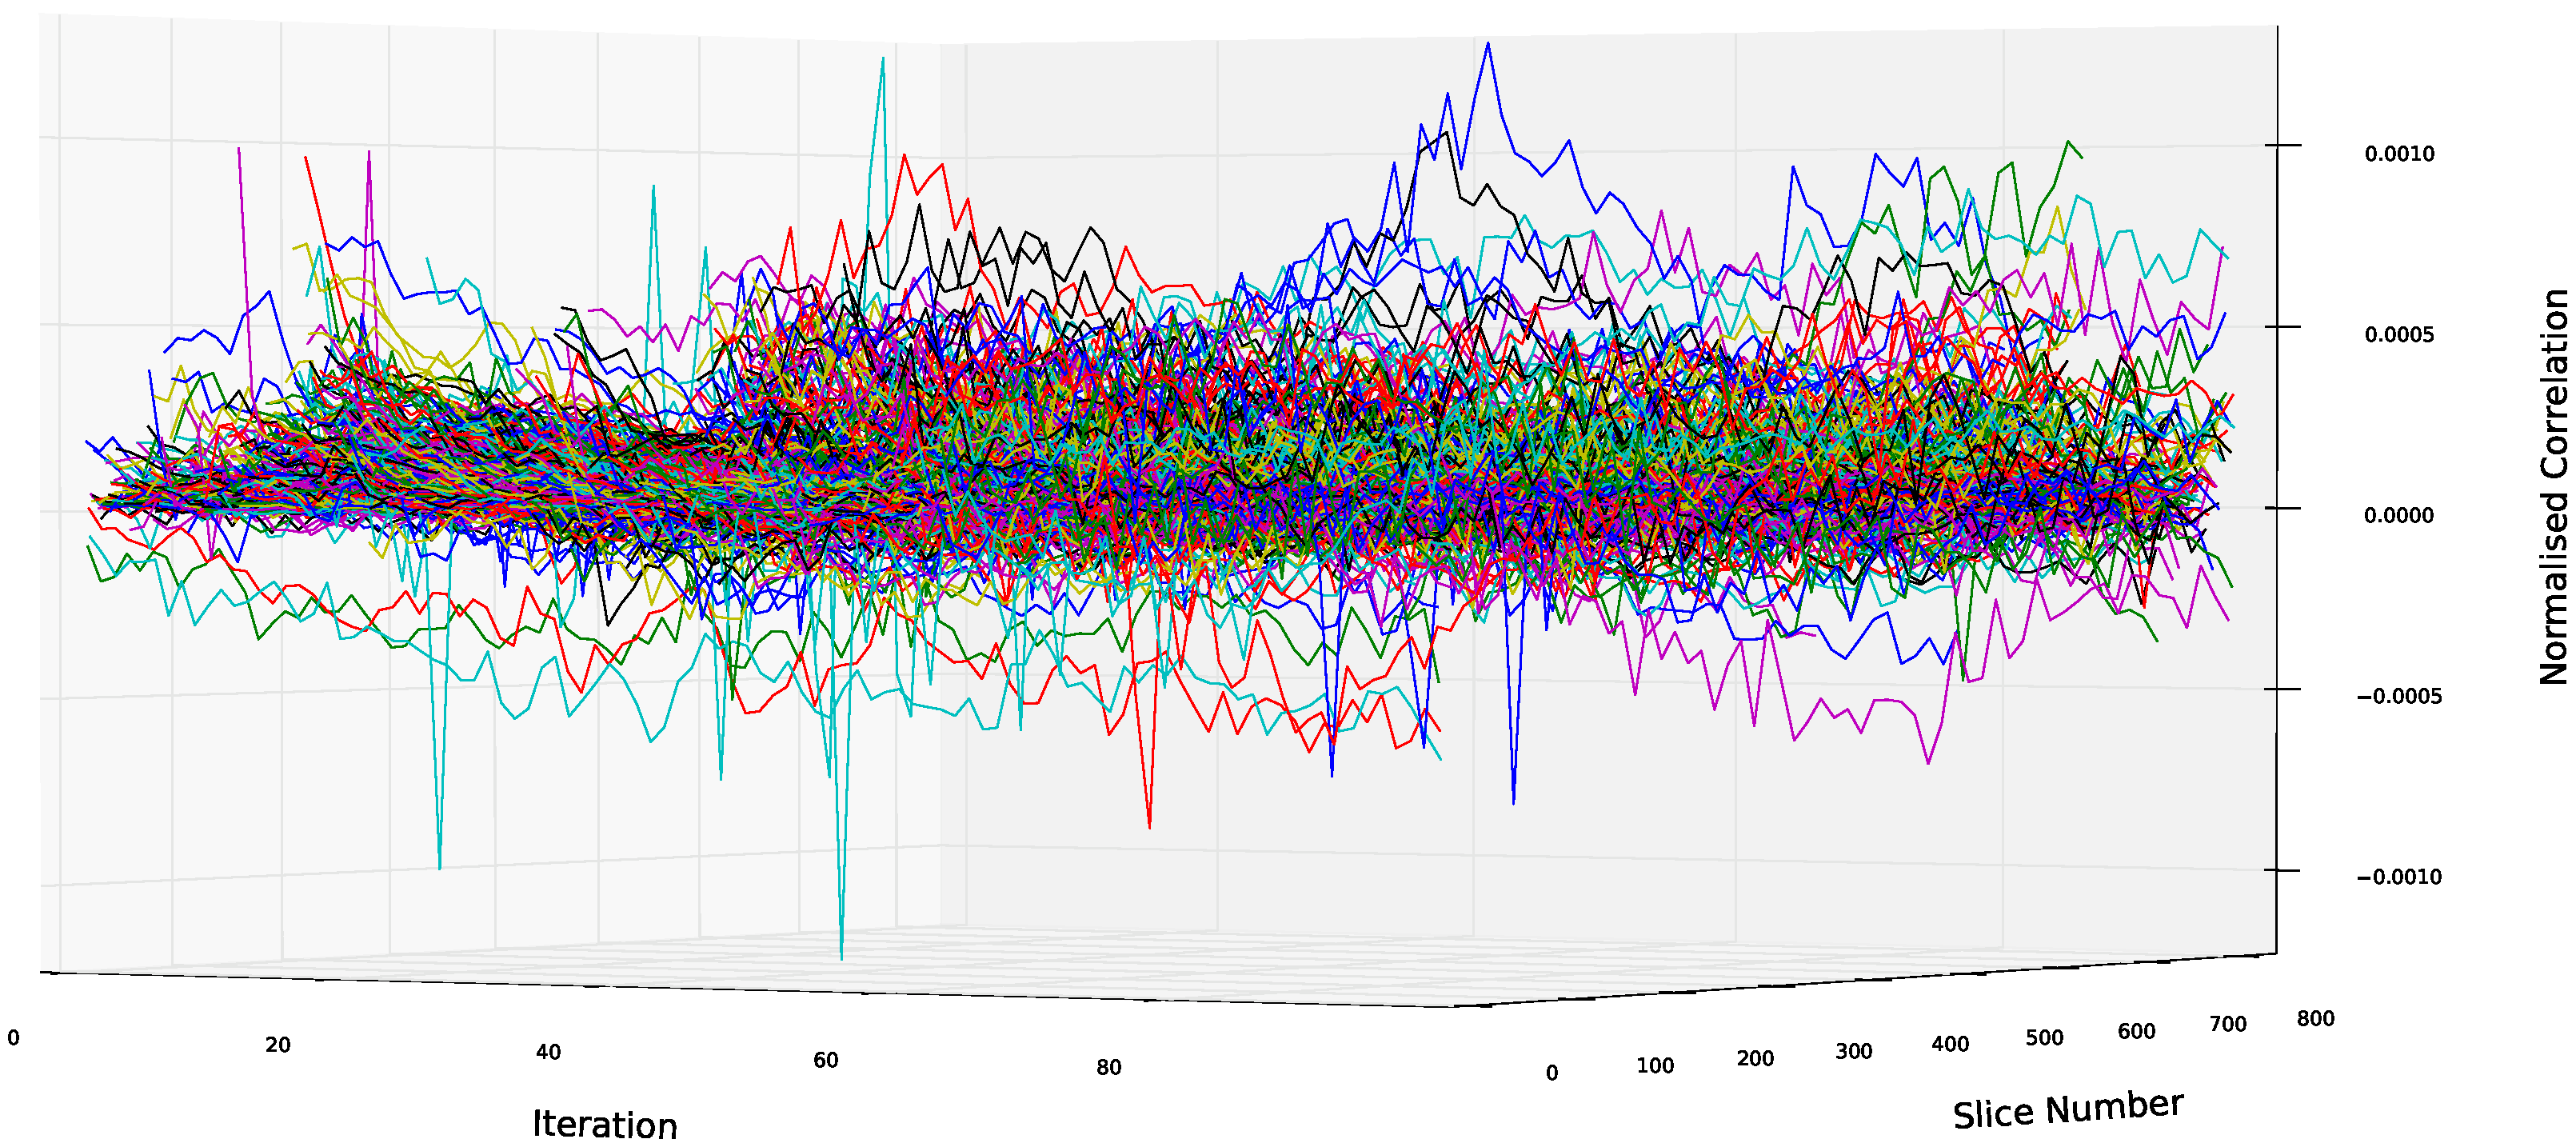
\includegraphics[width=\textheight]{Ch6/Figs/diagnostics/affine_metric_value_differences}
        \caption{}
        \label{fig:affine_metric_value_differences}
      \end{sidewaysfigure}
      
      \begin{sidewaysfigure}[htbp]
        \centering
        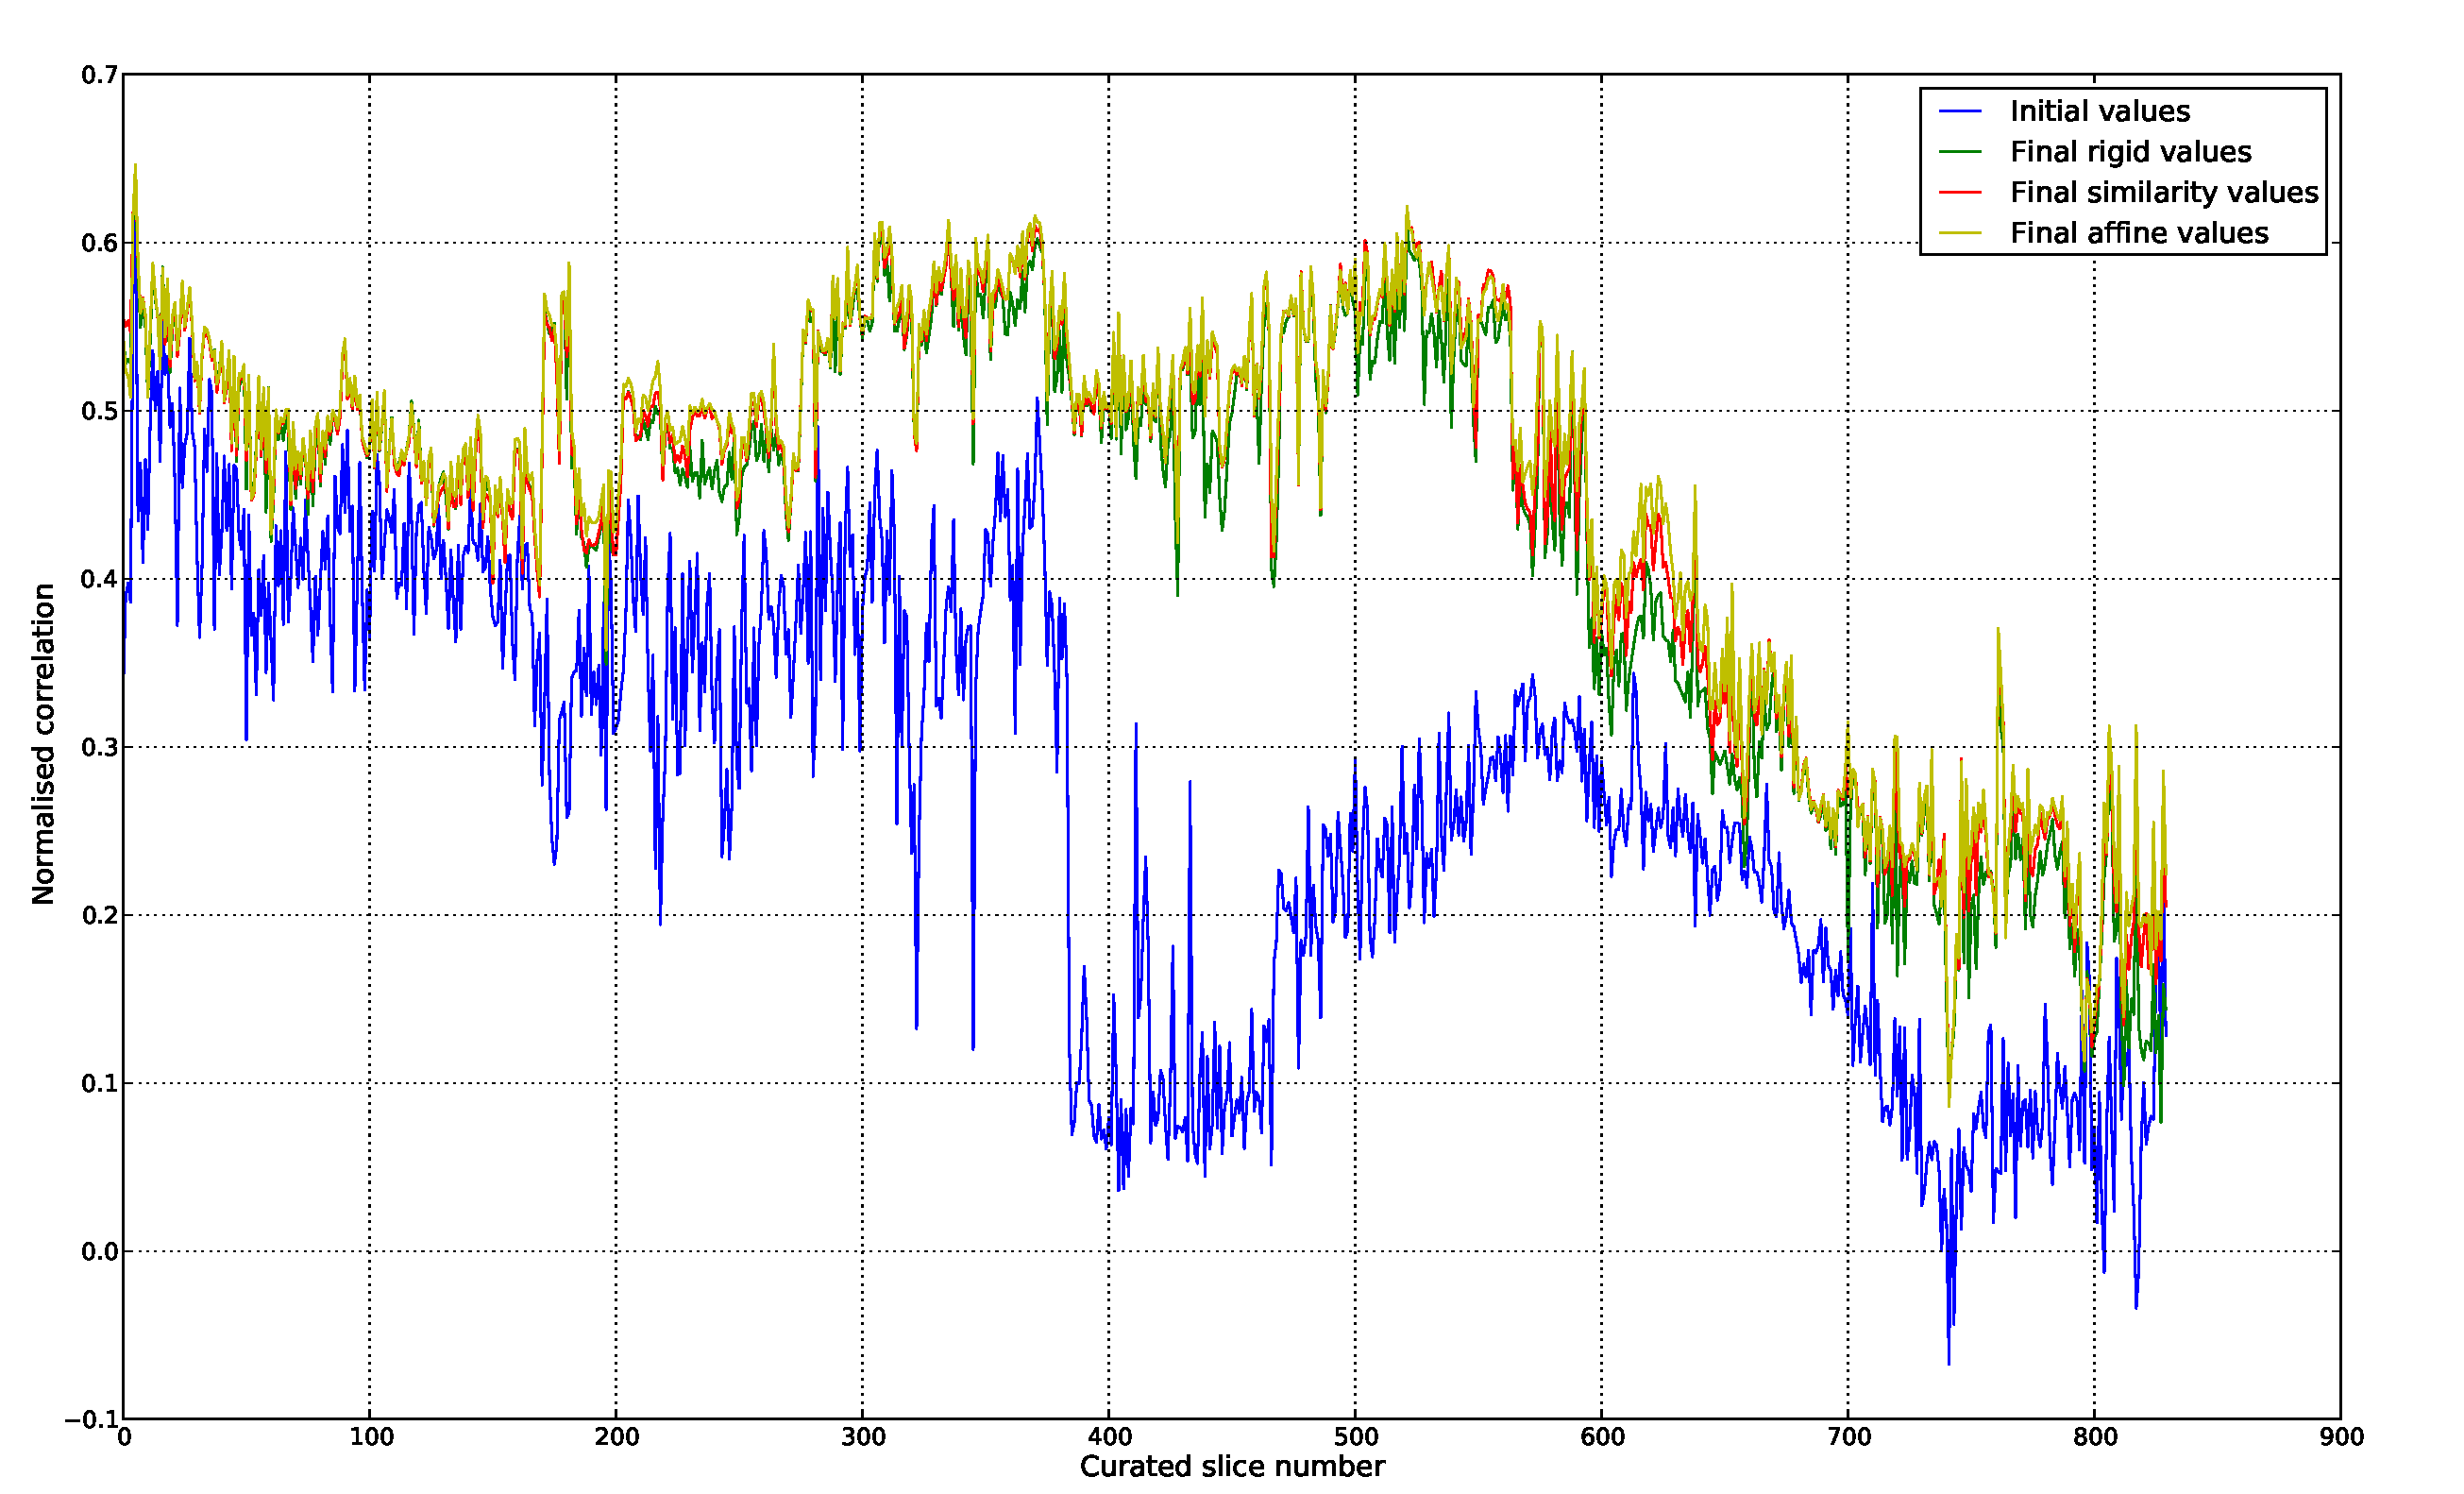
\includegraphics[width=\textheight]{Ch6/Figs/diagnostics/initial_and_final_values_comparison}
        \caption{Each successive registration increases correlation, but it is clear that the vast majority of improvement comes from the rigid registration. PERHAPS MOVE THE FOLLOWING TEXT SOMEWHERE ELSE: slices from 380 to 600 were photographed at a larger angle from that of their block-face images, and this is reflected in a sharply reduced initial correlation value. From Slice 600 onwards, the blob precludes successful registration and both initial and final correlation values decline.}
        \label{fig:initial_and_final_values_comparison}
      \end{sidewaysfigure}
      
      \begin{figure}[htbp]
        \centering
        \subfigure[][]{
\includegraphics[height=0.3\textheight]{Ch6/Figs/diagnostics/fixed_progress_slice_0562_1_287.pdf}}
        \subfigure[][]{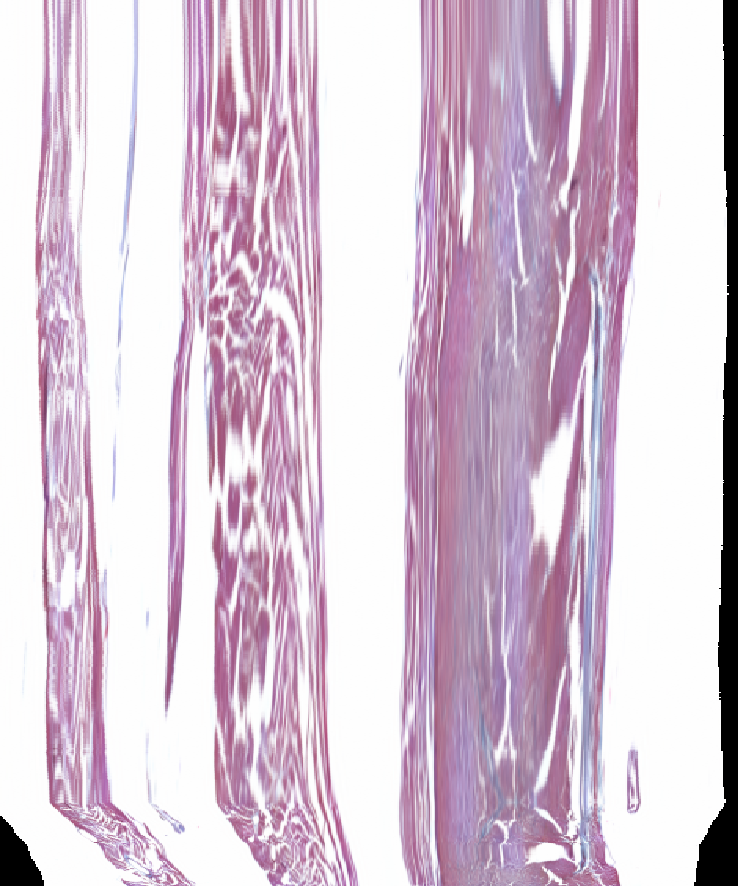
\includegraphics[height=0.3\textheight]{Ch6/Figs/diagnostics/moving_progress_slice_0562_1_287.pdf}}
        \subfigure[][]{
\includegraphics[height=0.3\textheight]{Ch6/Figs/diagnostics/fixed_progress_slice_0562_0_235.pdf}}
        \subfigure[][]{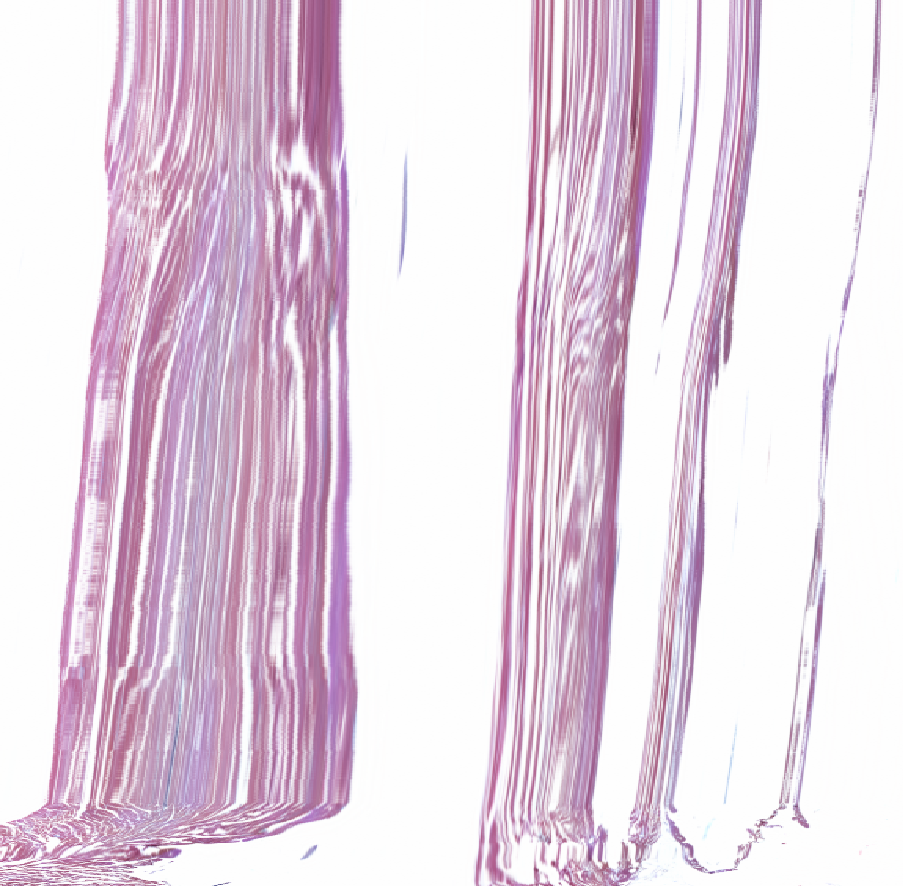
\includegraphics[height=0.3\textheight]{Ch6/Figs/diagnostics/moving_progress_slice_0562_0_235.pdf}}
        \caption{Progress volume of 1500 iterations of slice 0562}
        \label{fig:progress_cross_sections}
      \end{figure}
      
      \begin{figure}[htbp]
        \centering
        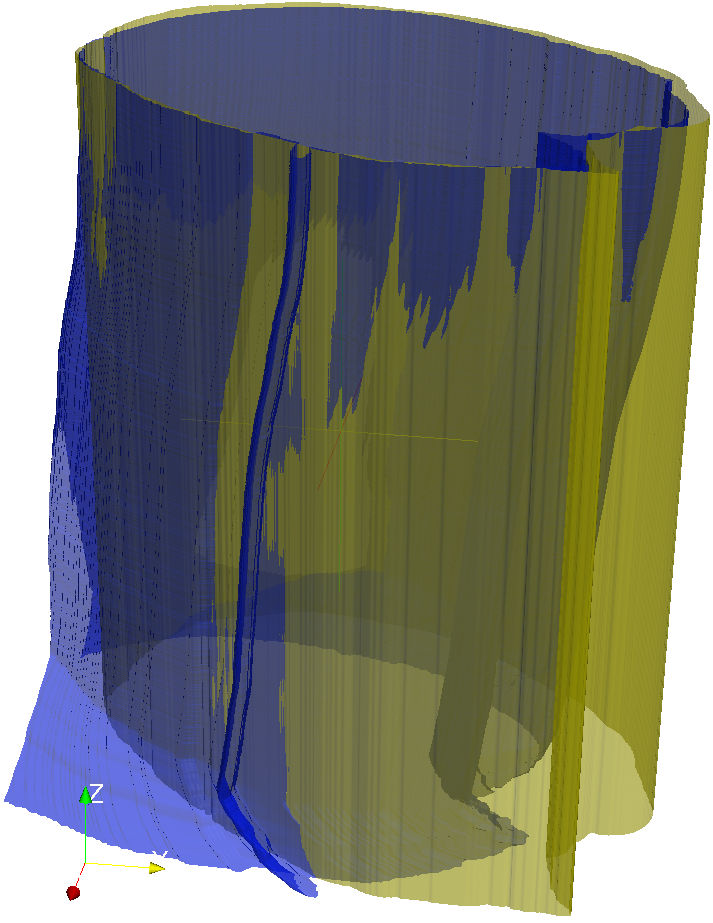
\includegraphics[width=\pagewidth]{Ch6/Figs/diagnostics/0562_contour.png}
        \caption{Quick rotation at the start, then flatter, slower translation...finally reaches a stationary minimum in the last iterations.}
        \label{fig:progress_contour}
      \end{figure}
      
      \begin{figure}[p]
        \centering
        \subfigure[][]{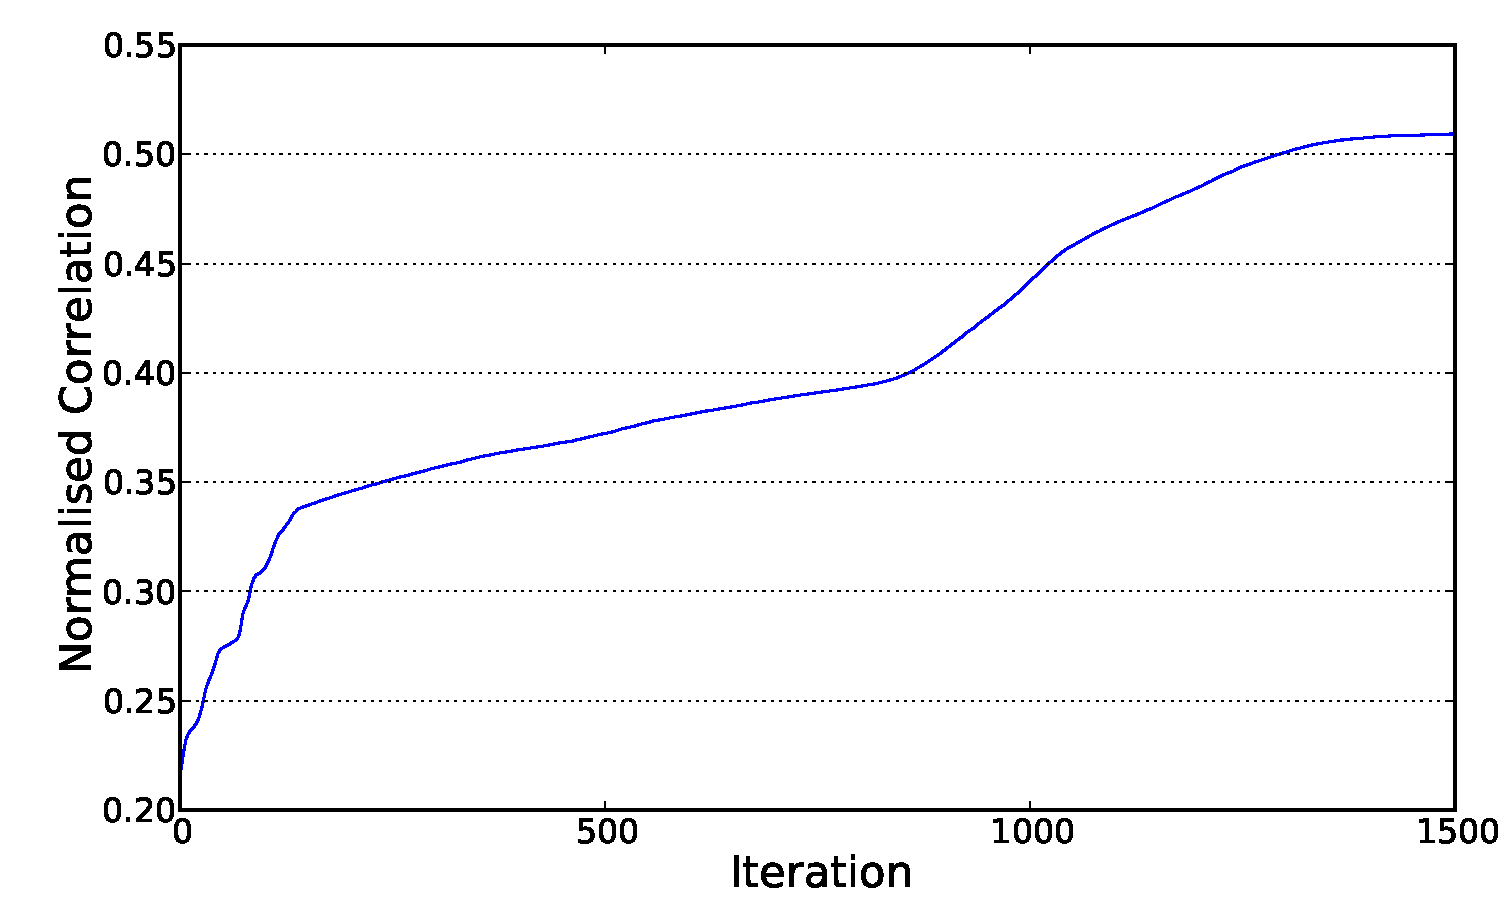
\includegraphics[width=0.9\pagewidth]{Ch6/Figs/diagnostics/0562_correlation}}
        \subfigure[][]{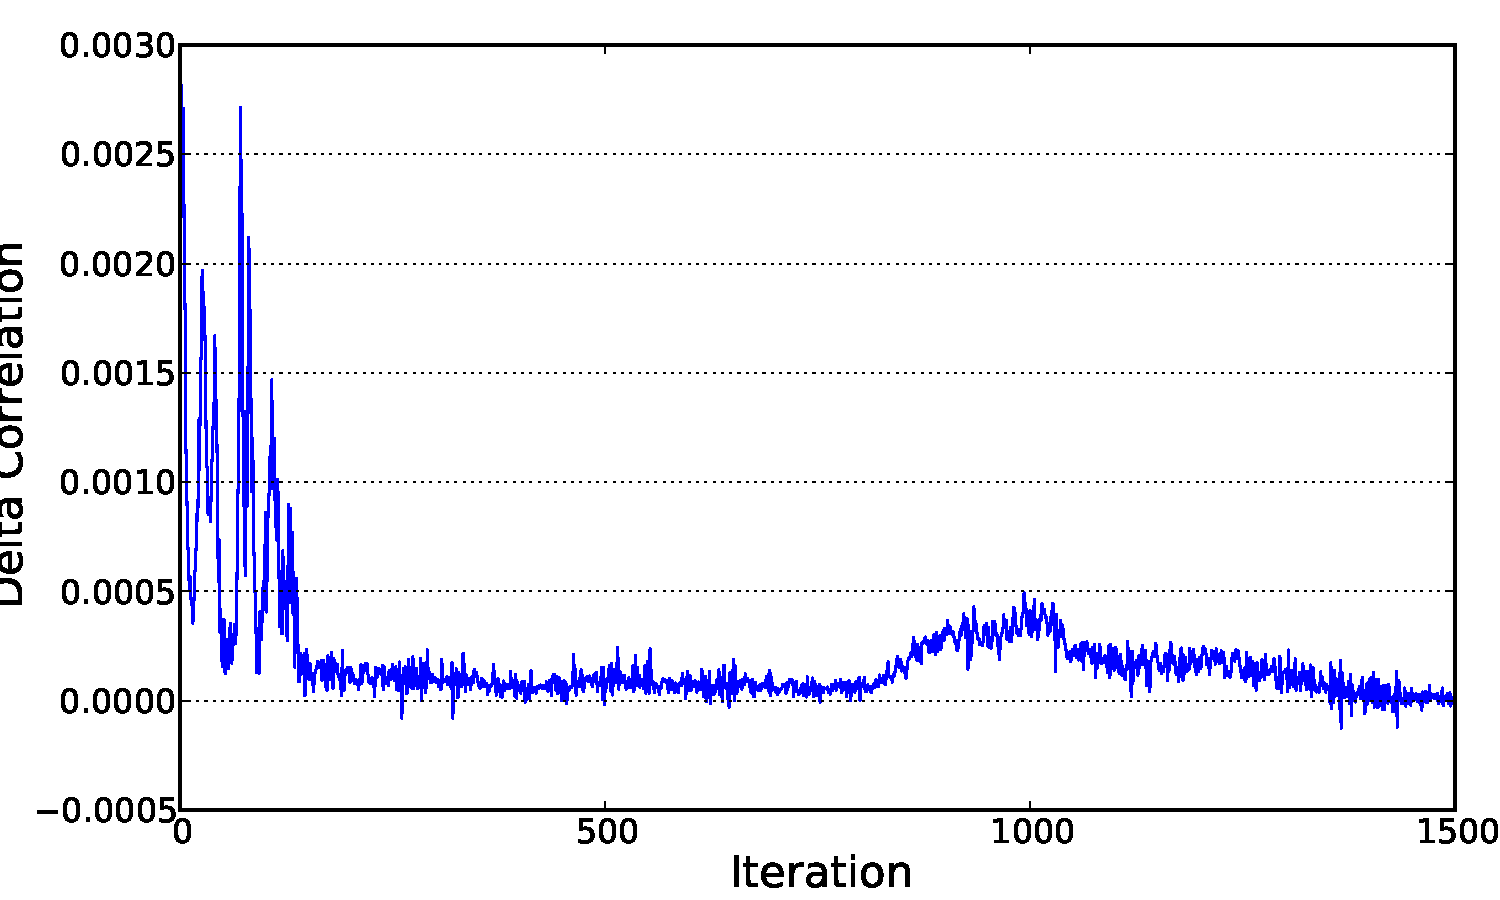
\includegraphics[width=0.9\pagewidth]{Ch6/Figs/diagnostics/0562_delta_correlation}}
        \caption{What a nice figure!}
        \label{fig:0562_correlation}
      \end{figure}
      
      
    % subsection diagnostics (end)
% section methods (end)
   
\section{Results}
  A series of figures will provide visual validation of the results, both of the full heart and more detailed images in regions of interest. Cross-sectional images perpendicular to the slice planes will show the close matching between planes, and segmented surfaces of myocardial walls and larger arteries will be rendered in 3-D. The performance of various registration regimes will be compared.
CONFIRMATION REPORT

% initialisation figure
\begin{sidewaysfigure}[htbp]
  \centering
  \subfigure[][]{
\includegraphics[height=0.31\textheight]{Ch6/Figs/geometric_0_235}}
  \subfigure[][]{
\includegraphics[height=0.31\textheight]{Ch6/Figs/geometric_1_287}}
  \caption{}
  \label{fig:geometric_initialisation}
\end{sidewaysfigure}

% x slices
\begin{figure}[htbp]
  \centering
  \subfigure[][]{
\includegraphics[height=0.31\textheight]{Ch6/Figs/rigid_0_235}}
  \subfigure[][]{
\includegraphics[height=0.31\textheight]{Ch6/Figs/size_0_235}}
  \subfigure[][]{
\includegraphics[height=0.31\textheight]{Ch6/Figs/affine_0_235}}
  \caption{Talk about how discontinuities in intensity between slices in the LoRes cutthrough fig are mirrored in the registration}
  \label{fig:hires_0_235}
\end{figure}

% y slices
\begin{figure}[htbp]
  \centering
  \subfigure[][]{
\includegraphics[height=0.31\textheight]{Ch6/Figs/rigid_1_287}}
  \subfigure[][]{
\includegraphics[height=0.31\textheight]{Ch6/Figs/size_1_287}}
  \subfigure[][]{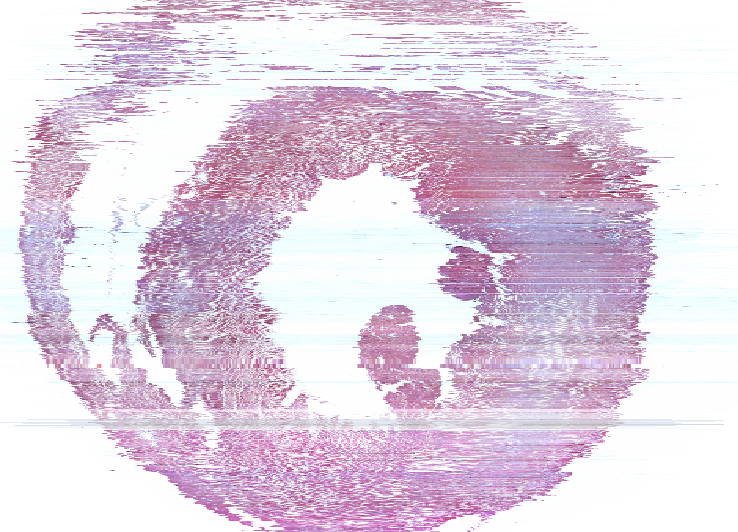
\includegraphics[height=0.31\textheight]{Ch6/Figs/affine_1_287}}
  \caption{What a nice figure!}
  \label{fig:hires_1_287}
\end{figure}

blah blah

blah blah

blah blah

blah blah

blah blah

blah blah

blah blah

blah blah

blah blah

blah blah

blah blah

blah blah

blah blah

blah blah

blah blah

blah blah

blah blah

blah blah

blah blah

blah blah

blah blah

blah blah

blah blah

blah blah

% geometric contours
\begin{sidewaysfigure}[p]
  \centering
  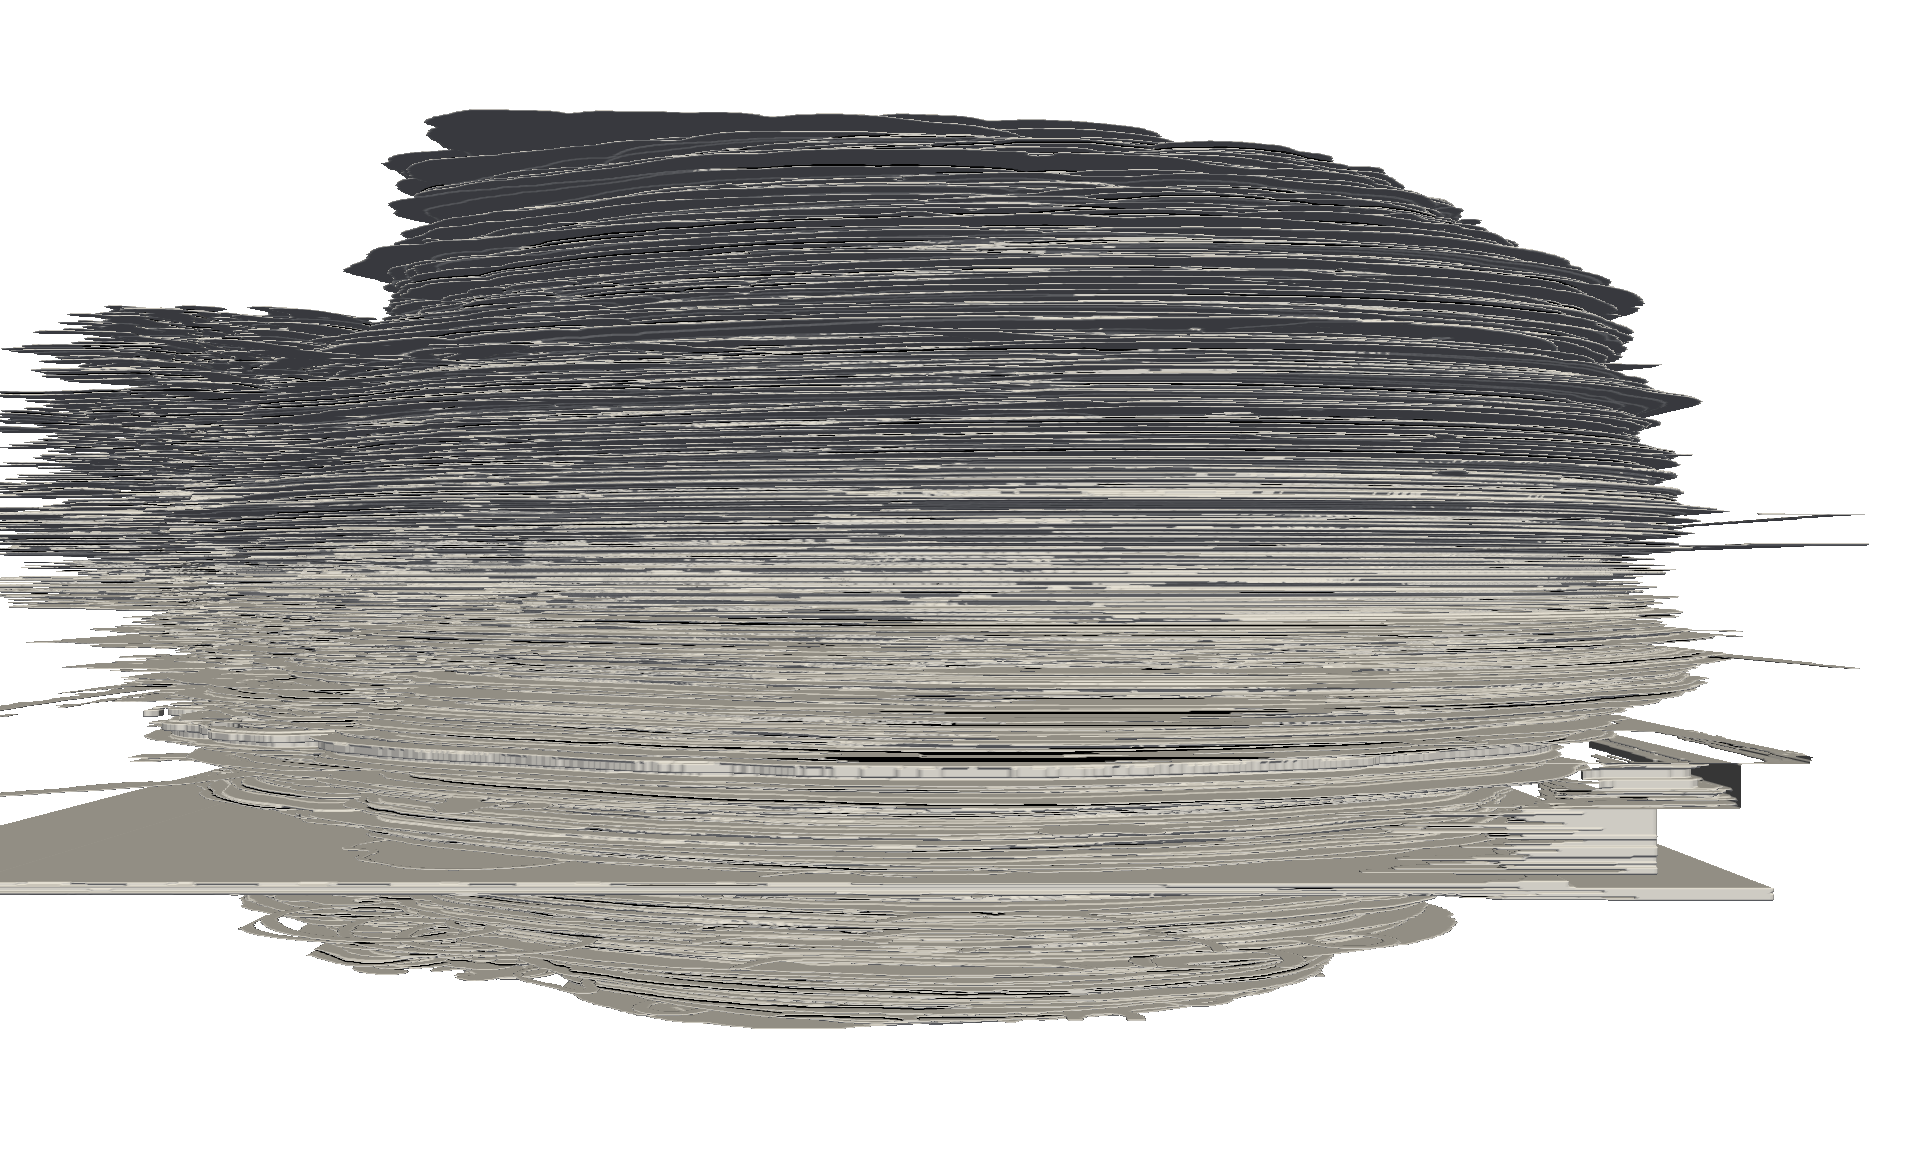
\includegraphics[width=0.9\textheight]{Ch7/Figs/Rat28/contours/whole_positive_x_geometric}
  \caption{Contour details: threshold segmentation with limits:0 to 240, used original slice images that were Gaussian smoothed by a kernel of std dev 64, because the detail from a simple threshold on nonsmoothed images generated egregiously convoluted surfaces. Because this smoothing only operates within the plane of the slices, individual displacements between edges of adjacent slices is still clearly visible. After segmentation, a label map filter was applied to remove all but the largest connected component. This went some way to removing bubbles and other artefacts obscuring the surface of the heart. y-dimension of geometry bounding box is extended from 575 to 700 to encompass the increased spread of the slices.}
  \label{fig:image1.png}
\end{sidewaysfigure}

\begin{sidewaysfigure}[p]
  \centering
  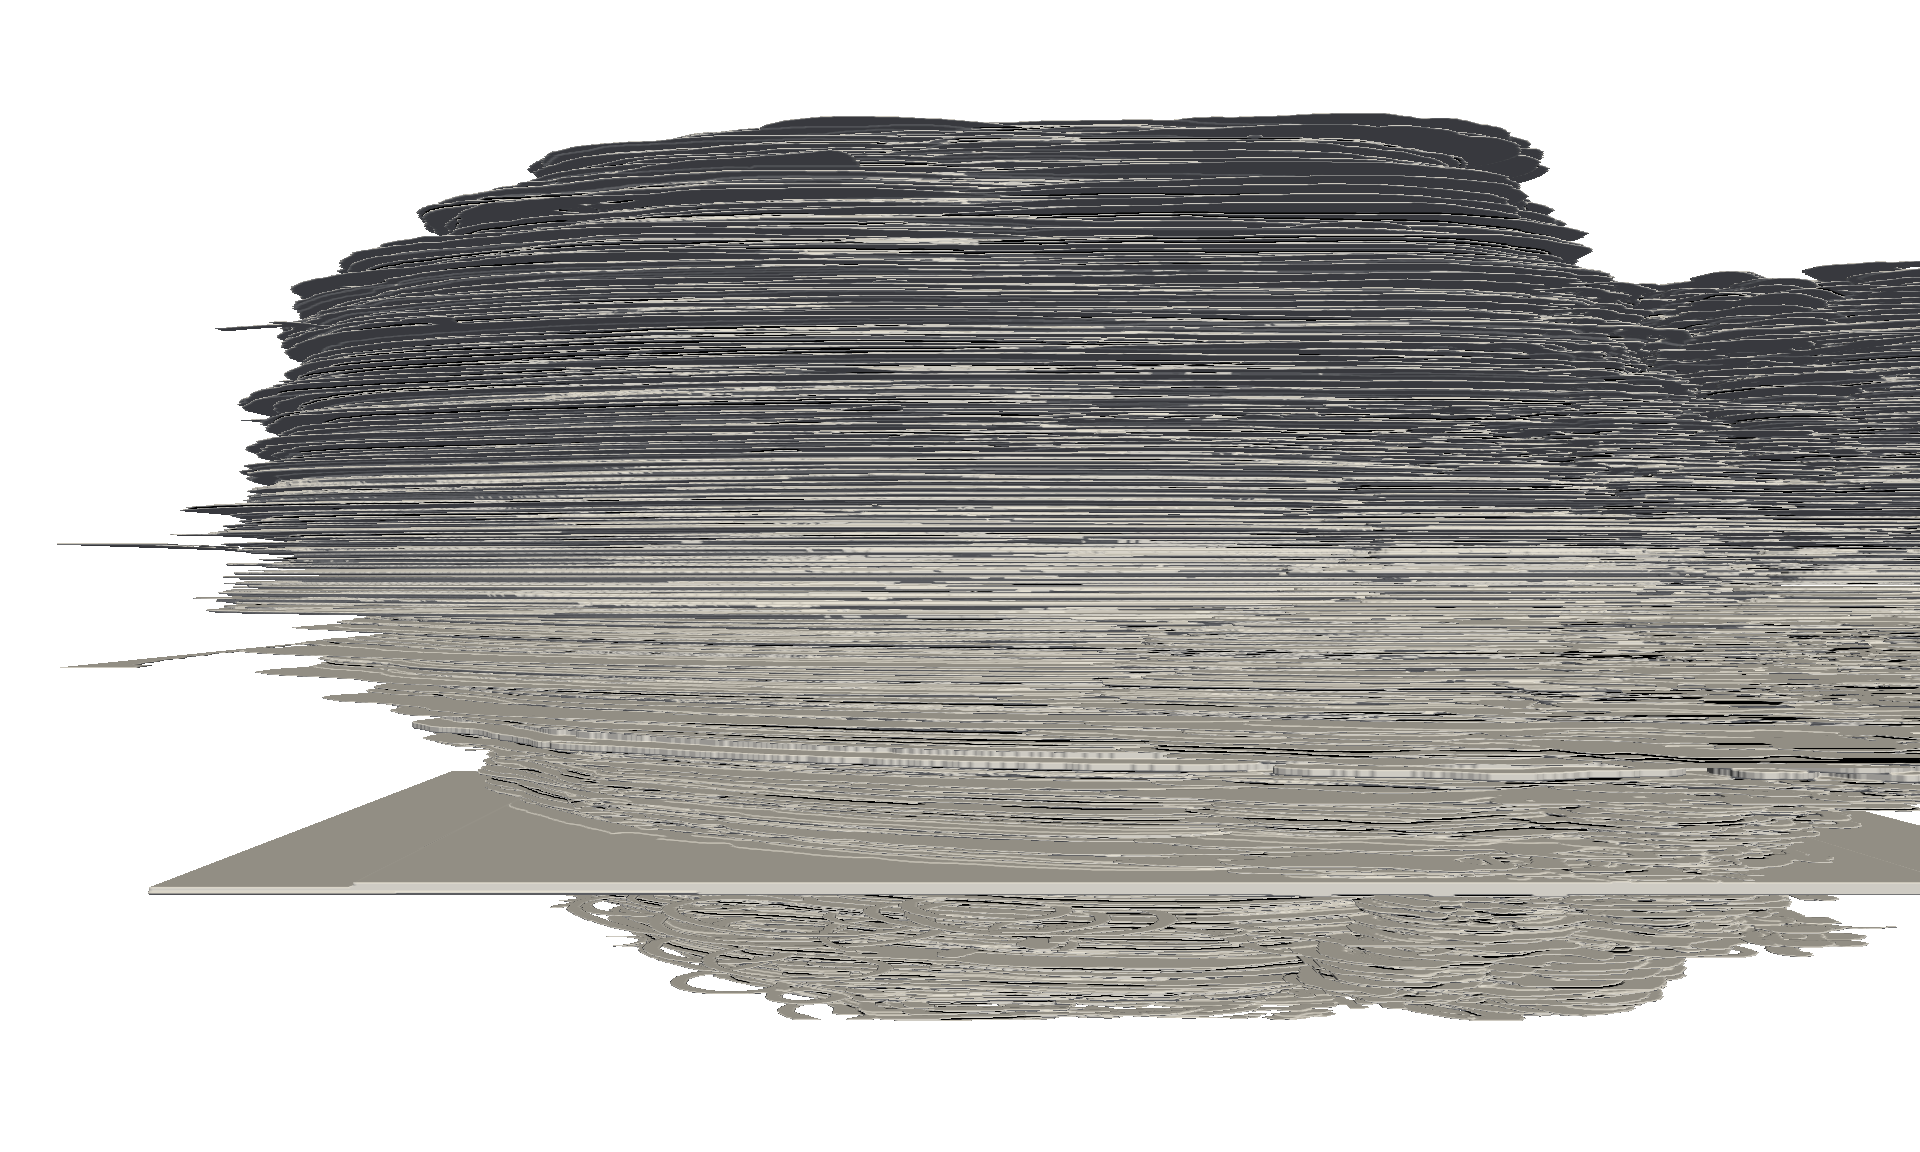
\includegraphics[width=0.9\textheight]{Ch7/Figs/Rat28/contours/whole_negative_x_geometric}
  \caption{}
  \label{fig:image1.png}
\end{sidewaysfigure}

\begin{sidewaysfigure}[p]
  \centering
  \includegraphics[width=0.9\textheight]{Ch7/Figs/Rat28/contours/whole_positive_y_geometric}
  \caption{}
  \label{fig:image1.png}
\end{sidewaysfigure}

\begin{sidewaysfigure}[p]
  \centering
  \includegraphics[width=0.9\textheight]{Ch7/Figs/Rat28/contours/whole_positive_z_geometric}
  \caption{}
  \label{fig:image1.png}
\end{sidewaysfigure}

% rigid contours
\begin{sidewaysfigure}[p]
  \centering
  \includegraphics[width=0.9\textheight]{Ch7/Figs/Rat28/contours/whole_positive_x_rigid}
  \caption{}
  \label{fig:image1.png}
\end{sidewaysfigure}

\begin{sidewaysfigure}[p]
  \centering
  \includegraphics[width=0.9\textheight]{Ch7/Figs/Rat28/contours/whole_negative_x_rigid}
  \caption{}
  \label{fig:image1.png}
\end{sidewaysfigure}

\begin{sidewaysfigure}[p]
  \centering
  \includegraphics[width=0.9\textheight]{Ch7/Figs/Rat28/contours/whole_positive_y_rigid}
  \caption{}
  \label{fig:image1.png}
\end{sidewaysfigure}

\begin{sidewaysfigure}[p]
  \centering
  \includegraphics[width=0.9\textheight]{Ch7/Figs/Rat28/contours/whole_positive_z_rigid}
  \caption{}
  \label{fig:image1.png}
\end{sidewaysfigure}

% size contours
\begin{sidewaysfigure}[p]
  \centering
  \includegraphics[width=0.9\textheight]{Ch7/Figs/Rat28/contours/whole_positive_x_size}
  \caption{}
  \label{fig:image1.png}
\end{sidewaysfigure}

\begin{sidewaysfigure}[p]
  \centering
  \includegraphics[width=0.9\textheight]{Ch7/Figs/Rat28/contours/whole_negative_x_size}
  \caption{}
  \label{fig:image1.png}
\end{sidewaysfigure}

\begin{sidewaysfigure}[p]
  \centering
  \includegraphics[width=0.9\textheight]{Ch7/Figs/Rat28/contours/whole_positive_y_size}
  \caption{}
  \label{fig:image1.png}
\end{sidewaysfigure}

\begin{sidewaysfigure}[p]
  \centering
  \includegraphics[width=0.9\textheight]{Ch7/Figs/Rat28/contours/whole_positive_z_size}
  \caption{}
  \label{fig:image1.png}
\end{sidewaysfigure}

% affine contours
\begin{sidewaysfigure}[p]
  \centering
  \includegraphics[width=0.9\textheight]{Ch7/Figs/Rat28/contours/whole_positive_x_affine}
  \caption{}
  \label{fig:image1.png}
\end{sidewaysfigure}

\begin{sidewaysfigure}[p]
  \centering
  \includegraphics[width=0.9\textheight]{Ch7/Figs/Rat28/contours/whole_negative_x_affine}
  \caption{}
  \label{fig:image1.png}
\end{sidewaysfigure}

\begin{sidewaysfigure}[p]
  \centering
  \includegraphics[width=0.9\textheight]{Ch7/Figs/Rat28/contours/whole_positive_y_affine}
  \caption{}
  \label{fig:image1.png}
\end{sidewaysfigure}

\begin{sidewaysfigure}[p]
  \centering
  \includegraphics[width=0.9\textheight]{Ch7/Figs/Rat28/contours/whole_positive_z_affine}
  \caption{}
  \label{fig:image1.png}
\end{sidewaysfigure}


\section{Discussion} % (fold)
\label{sec:discussion}

\textit{PROGRESS FROM CONFIRMATION REPORT 
A full-heart registration pipeline has been developed and downsampled histological volumes generated. An initial manual alignment is followed by rigid and similarity transforms. The quality of the registrations are quite poor at present, and the task at hand is to fine-tune the various parameters that constrain the process: parameter space preconditioning, maximum iterations, maximum and minimum step lengths, number of spatial samples and metric-specific parameters.
END PROGRESS FROM CONFIRMATION REPORT
}
    We have constructed a comprehensive, generic and flexible pipeline to register histological slices to block face images, that can be configured to generate rapid results on the broadest spectrum of computational facilities, from laptop to supercomputer.
    
    Talk about ad hoc meta-optimisation of registration parameters, could be more formalised but a great deal more effort and prone to error (e.g. mean final metric values of all slices might decrease, but end result may suck)
    
    The method for optimising registration parameters is a crude and intuitive version of the optimisation algorithms applied to the image registrations. Not easily possible to calculate gradient of metric in parameter space, but can perturb coordinates along basis axes e.g. parameter scaling, choice of metric or optimiser, gradient descent learning rate, RSGD relaxation factor, whether to normalise images etc. 2 approaches: could split the space into two groups of `preferred' axes, and secondary axes, then perform an (exhaustive?) prototype search in the preferred subspace, and for each preferred coordinate perform an iterative optimisation in the secondary space. Alternatively, just perform iterative stochastic search in the whole space.
    
    ?NEEDS DEVELOPMENT? Some params like choice of metric have different associated parameter spaces e.g. learning rate vs relaxation factor, and also are likely to lead to widely different optimal spaces along other axes e.g. parameter scaling.
    
    Problems about things like histogram matching, Mutual info: for histogram matching there is no monotonic mapping between the intensity in the lores and that of the hires, with tissue /non tissue. With Mutual info, doesn't need to be monotonic, but there isn't even a one-to-one mapping i.e. many regions of tissue in lores occupy the same intensity range as non-tissue.
    
    Conclude that experimental acquisition techniques have advanced since Rat28 was acquired, and some of the image processing techniques exposed here will perform much better with even higher quality and more homogeneous data.
    
    Dicuss why b-splines didn't work.
% section discussion (end)

REGISTRATION PAPER

% \input{../registration_paper/latex/methods/methods}
% \input{../registration_paper/latex/results/results}
  